\section{Previously, on DisCoCat}

DisCoCat is a research programme in applied mathematical linguistics that is \textbf{Dis}tributional, \textbf{Co}mpositional and \textbf{Cat}egorical. In this section I will recount a selective development of DisCoCat as relevant for this thesis.

\subsection{Lambek's Linguistics}

It's hard for me to do justice to Jim Lambek's life. I feel as if have been in intimate conversation with Jim throughout my research, despite our separation by time. Anyone can look up the Curry-Howard-Lambek correspondence and follow the rabbit hole to see Jim's broad reach and lasting impact on category theory. I know that he was a jovial man who always carried a good sense of humour and a wad of twenties. I also can't do better than Moortgat's history and exposition of typelogical grammar in \bR CITE \e, so I will borrow Moortgat's phrasing and summarise Lambek's role in the story. Typelogical grammar originated in two seminal papers by Lambek in 1958 and 1961 \bR CITE \e, where Lambek sought “to obtain an effective rule (or algorithm) for distinguishing sentences from non-sentences, which works not only for the formal languages of interest to the mathematical logician, but also for natural languages […]”. The method is to assign grammatical categories -- parts of speech such as nouns and verbs -- logical formulae. Whether a sentence is grammatical or not is obtained from deduction using these logical formulae in a Gentzen-style sequent proof.

\begin{figure}[h!]
\centering
\scalebox{1}{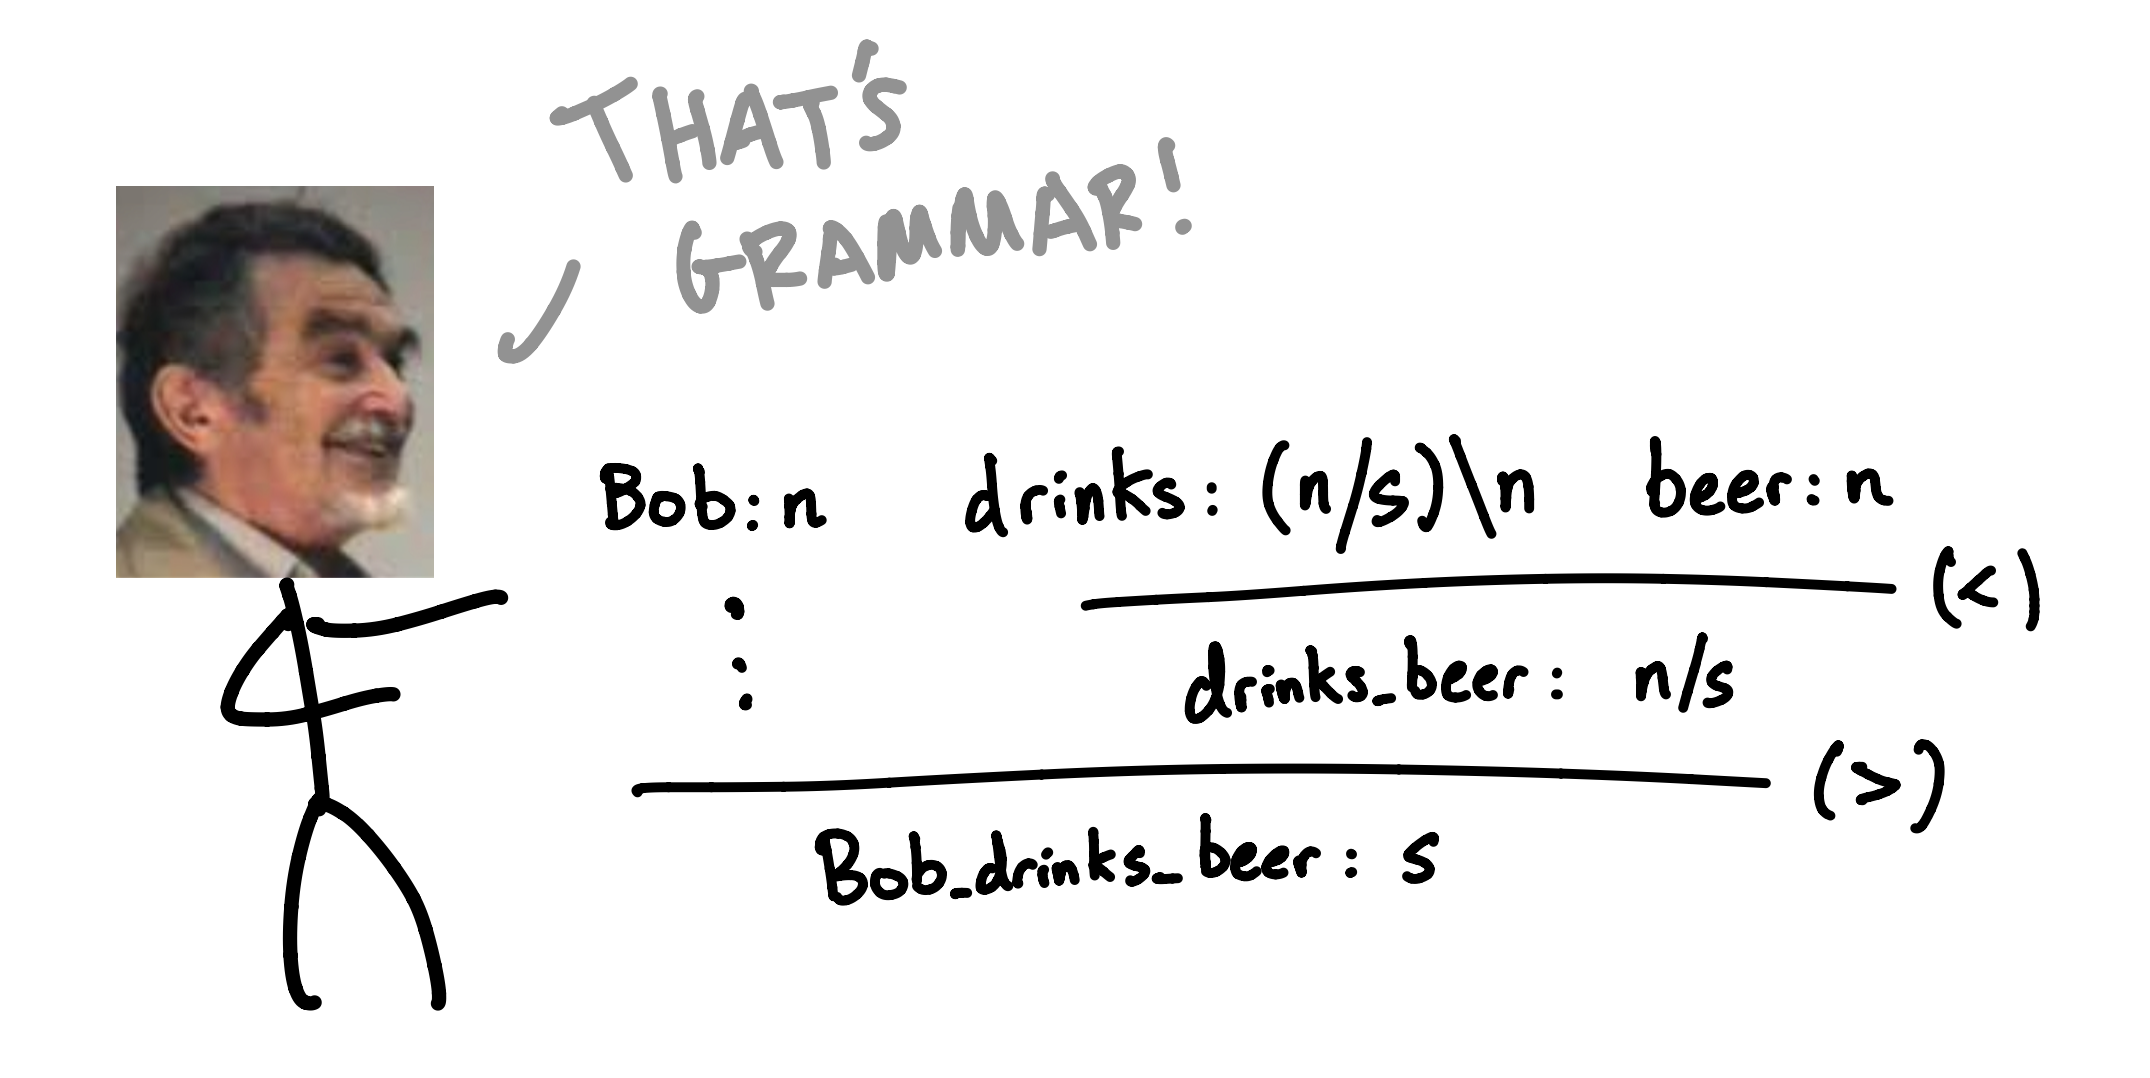
\includegraphics{figures/cartoons/lambek1}}
\caption{In English, we may consider a noun to have type $n$, and a transitive verb $(n/s)\setminus n$, to yield a well-formedness proof of \texttt{Bob drinks beer}. The type formation rules for such a grammar are intuitive. Apart from a stock of basic types $\mathbb{B}$ that contains special final types to indicate sentences, we have two type formation operators $(-/=)$ and $(- \setminus =)$, which along with their elimination rules establish a requirement that grammatical categories require other grammatical categories to their left or right. This is the essence of Lambek's calculi \textbf{NL} and \textbf{L}. CCGs keep the same minimal type-formations, but include extra sequent rules such as type-raising and cross-composition.}
\end{figure}

\begin{figure}[h!]
\centering
\scalebox{1}{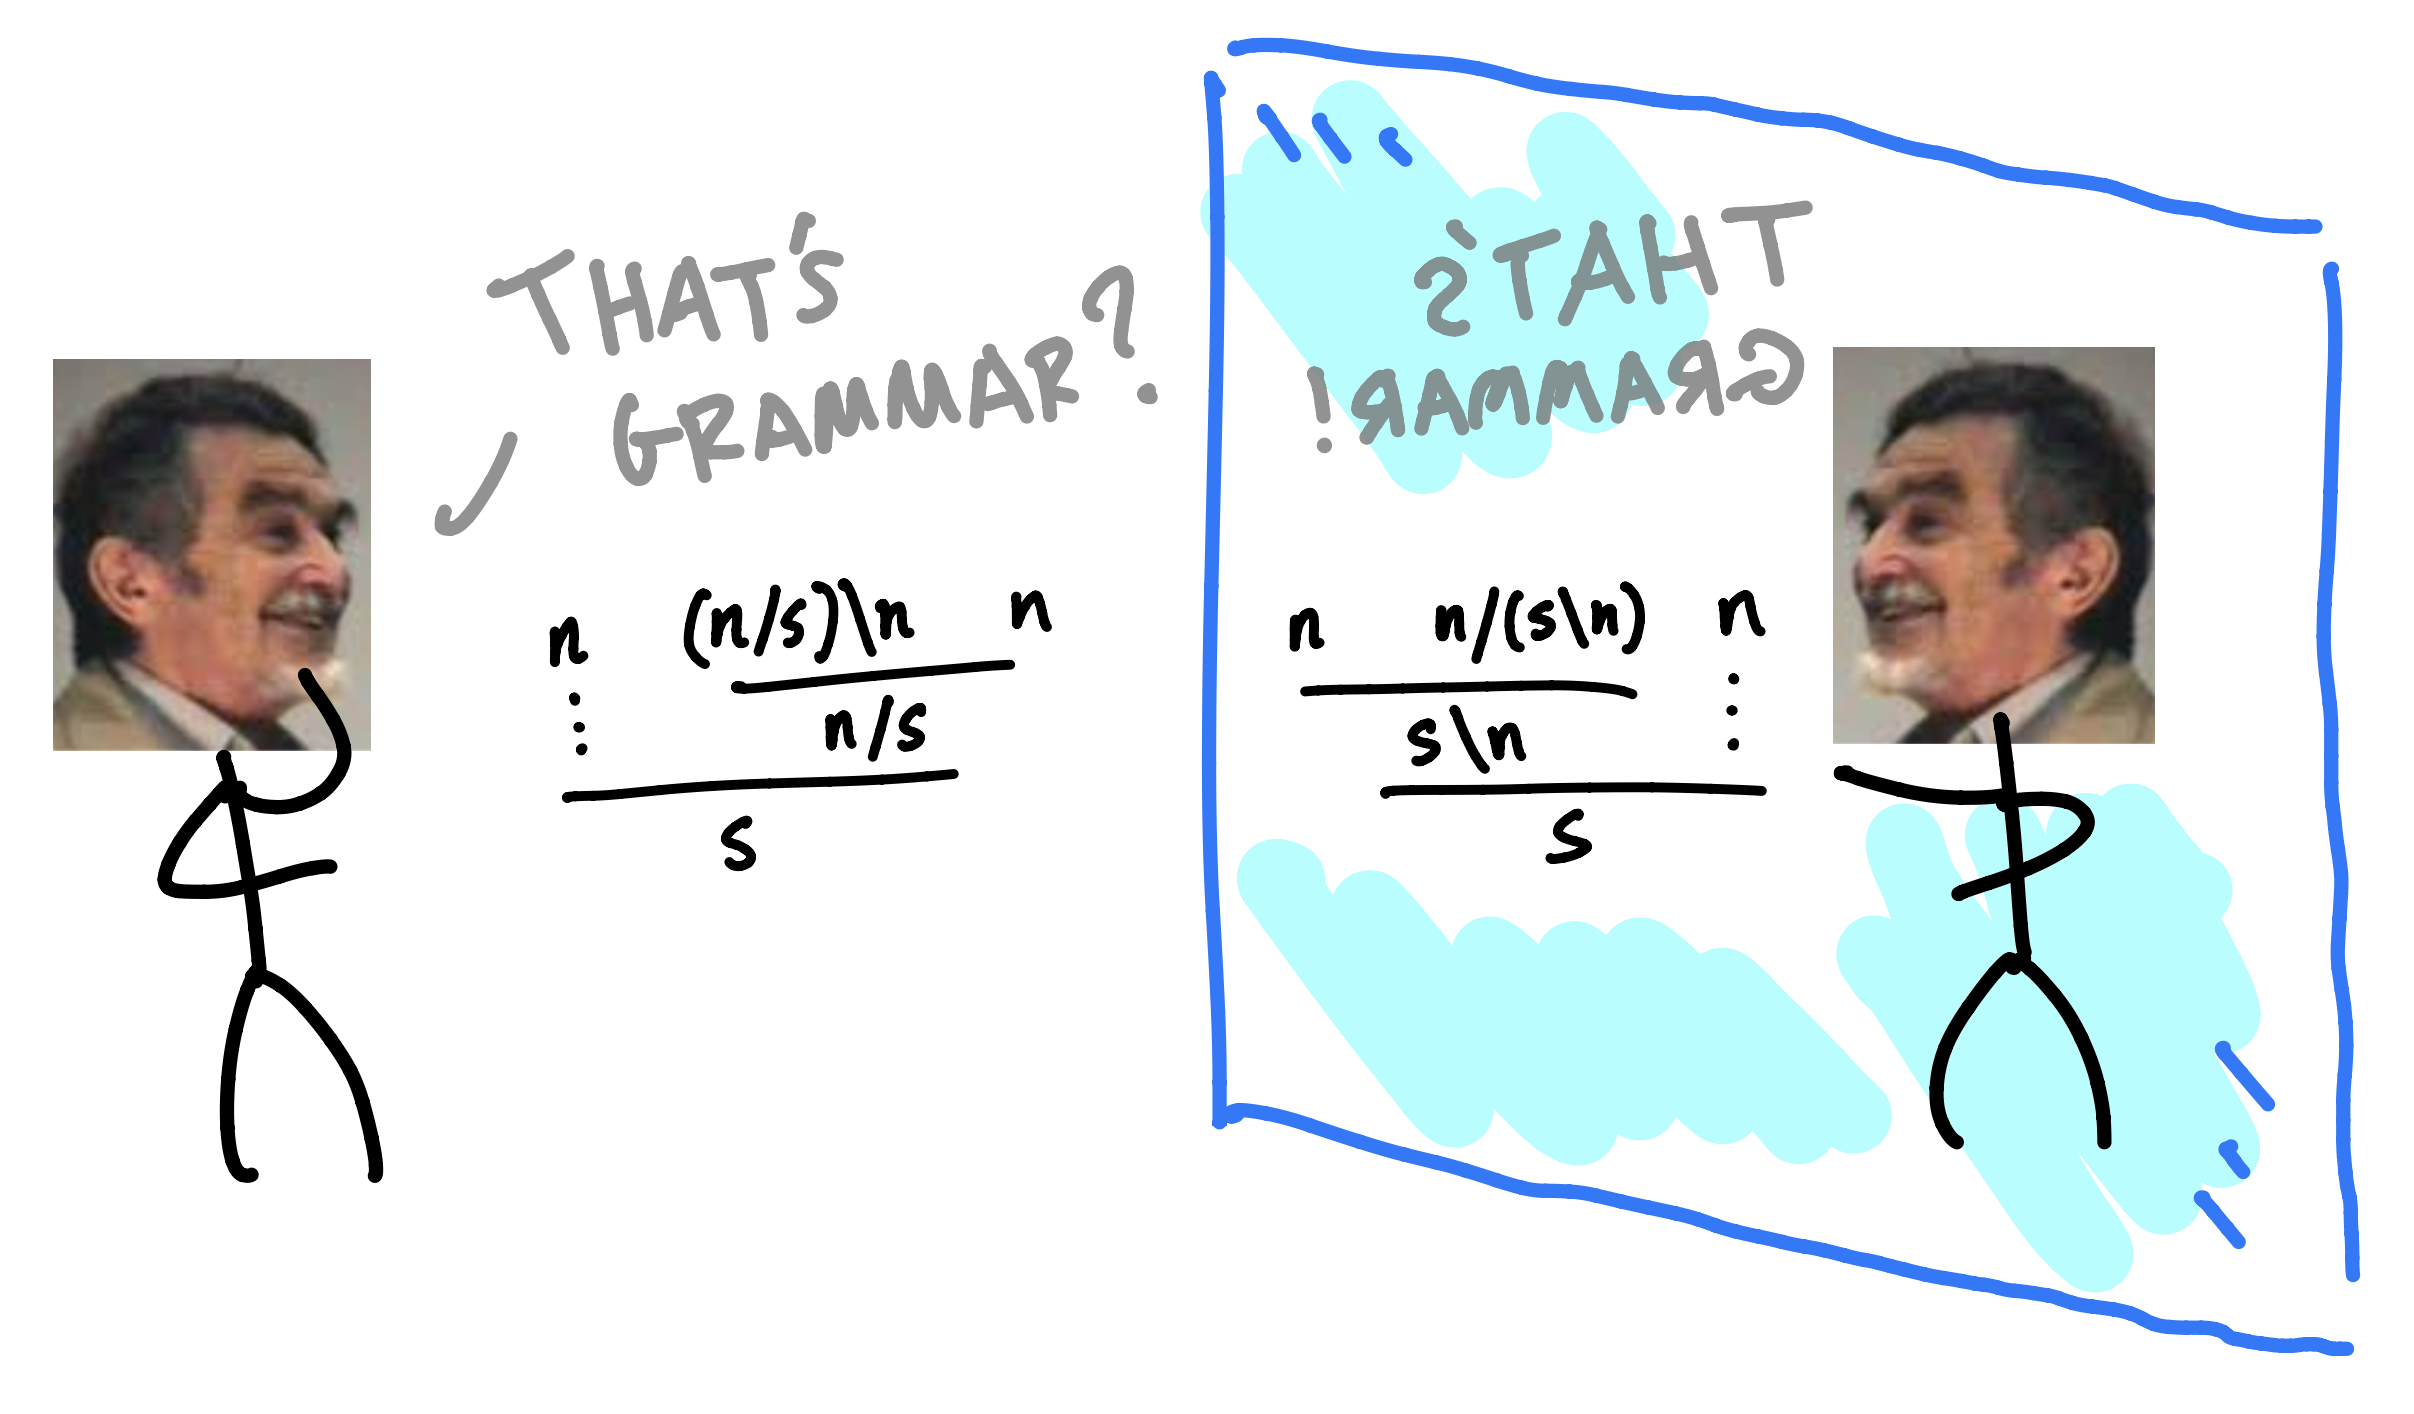
\includegraphics{figures/cartoons/lambek2}}
\caption{We can notice an asymmetry in the above formulation when we examine the transitive verb type $(n/s)\setminus n$ again; it asks first for a noun to the right, and then a noun to the left. We could just as well have asked for the nouns in the other order with the typing $(n/s)\setminus n$ and obtained all of the same proofs.}
\end{figure}

\begin{figure}[h!]
\centering
\scalebox{1}{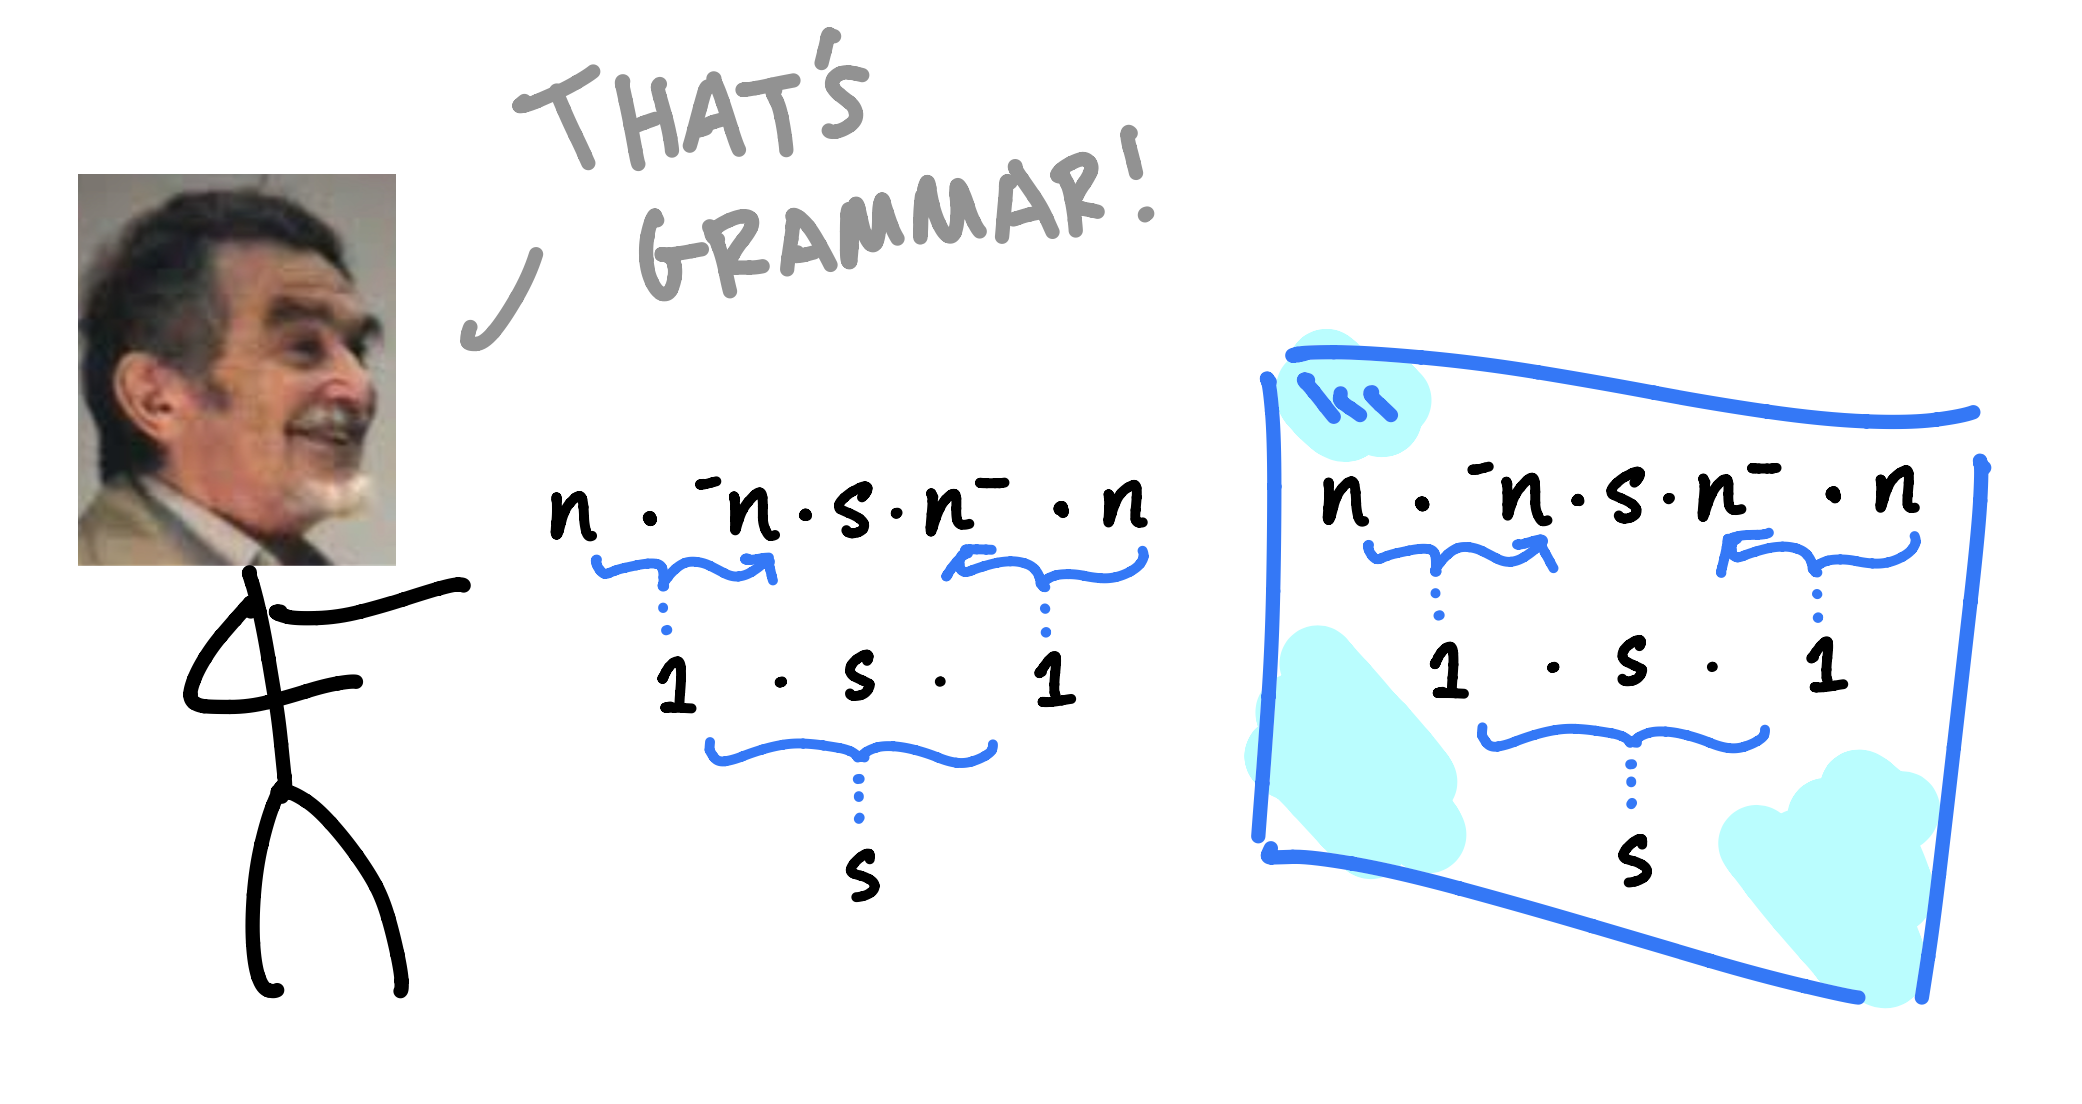
\includegraphics{figures/cartoons/lambek3}}
\caption{To eliminate this asymmetry, Lambek devised pregroup grammars. Whereas a group is a monoid with inverses up to left- and right-multiplication, a pregroup weakens the requirement for inverses so that all elements have distinct left- and right- inverses, denoted $x^{-1}$ and $^{-1}x$ respectively. Eliminating or introducing inverses is a non-identity relation on elements of the pregroup, so we have axioms of the form e.g. $x \cdot ^{-1}x \rightarrow 1 \rightarrow ^{1}x \cdot x$. In this formulation, denoting the multiplication with a dot, both $(n/s)\setminus n$ and $(n/s)\setminus n$ become $^{-1}n \cdot s \cdot n^{-1}$, which just wants a noun to the left and a noun to the right in whatever order to eliminate the flanking inverses to reveal the embedded sentence type. Now we can obtain the same proof of correctness as a series of algebraic reductions.

\begin{align*}
& &n \cdot (^{-1}n \cdot s \cdot n^{-1}) \cdot n\\
&\rightarrow &(n \cdot ^{-1}n) \cdot s \cdot (n^{-1} \cdot n)\\
&\rightarrow & 1 \cdot s \cdot 1\\
&\rightarrow & s
\end{align*}
}
\end{figure}
\clearpage

\subsection{Coecke's Composition}

\begin{figure}[h!]
\centering
\scalebox{0.9}{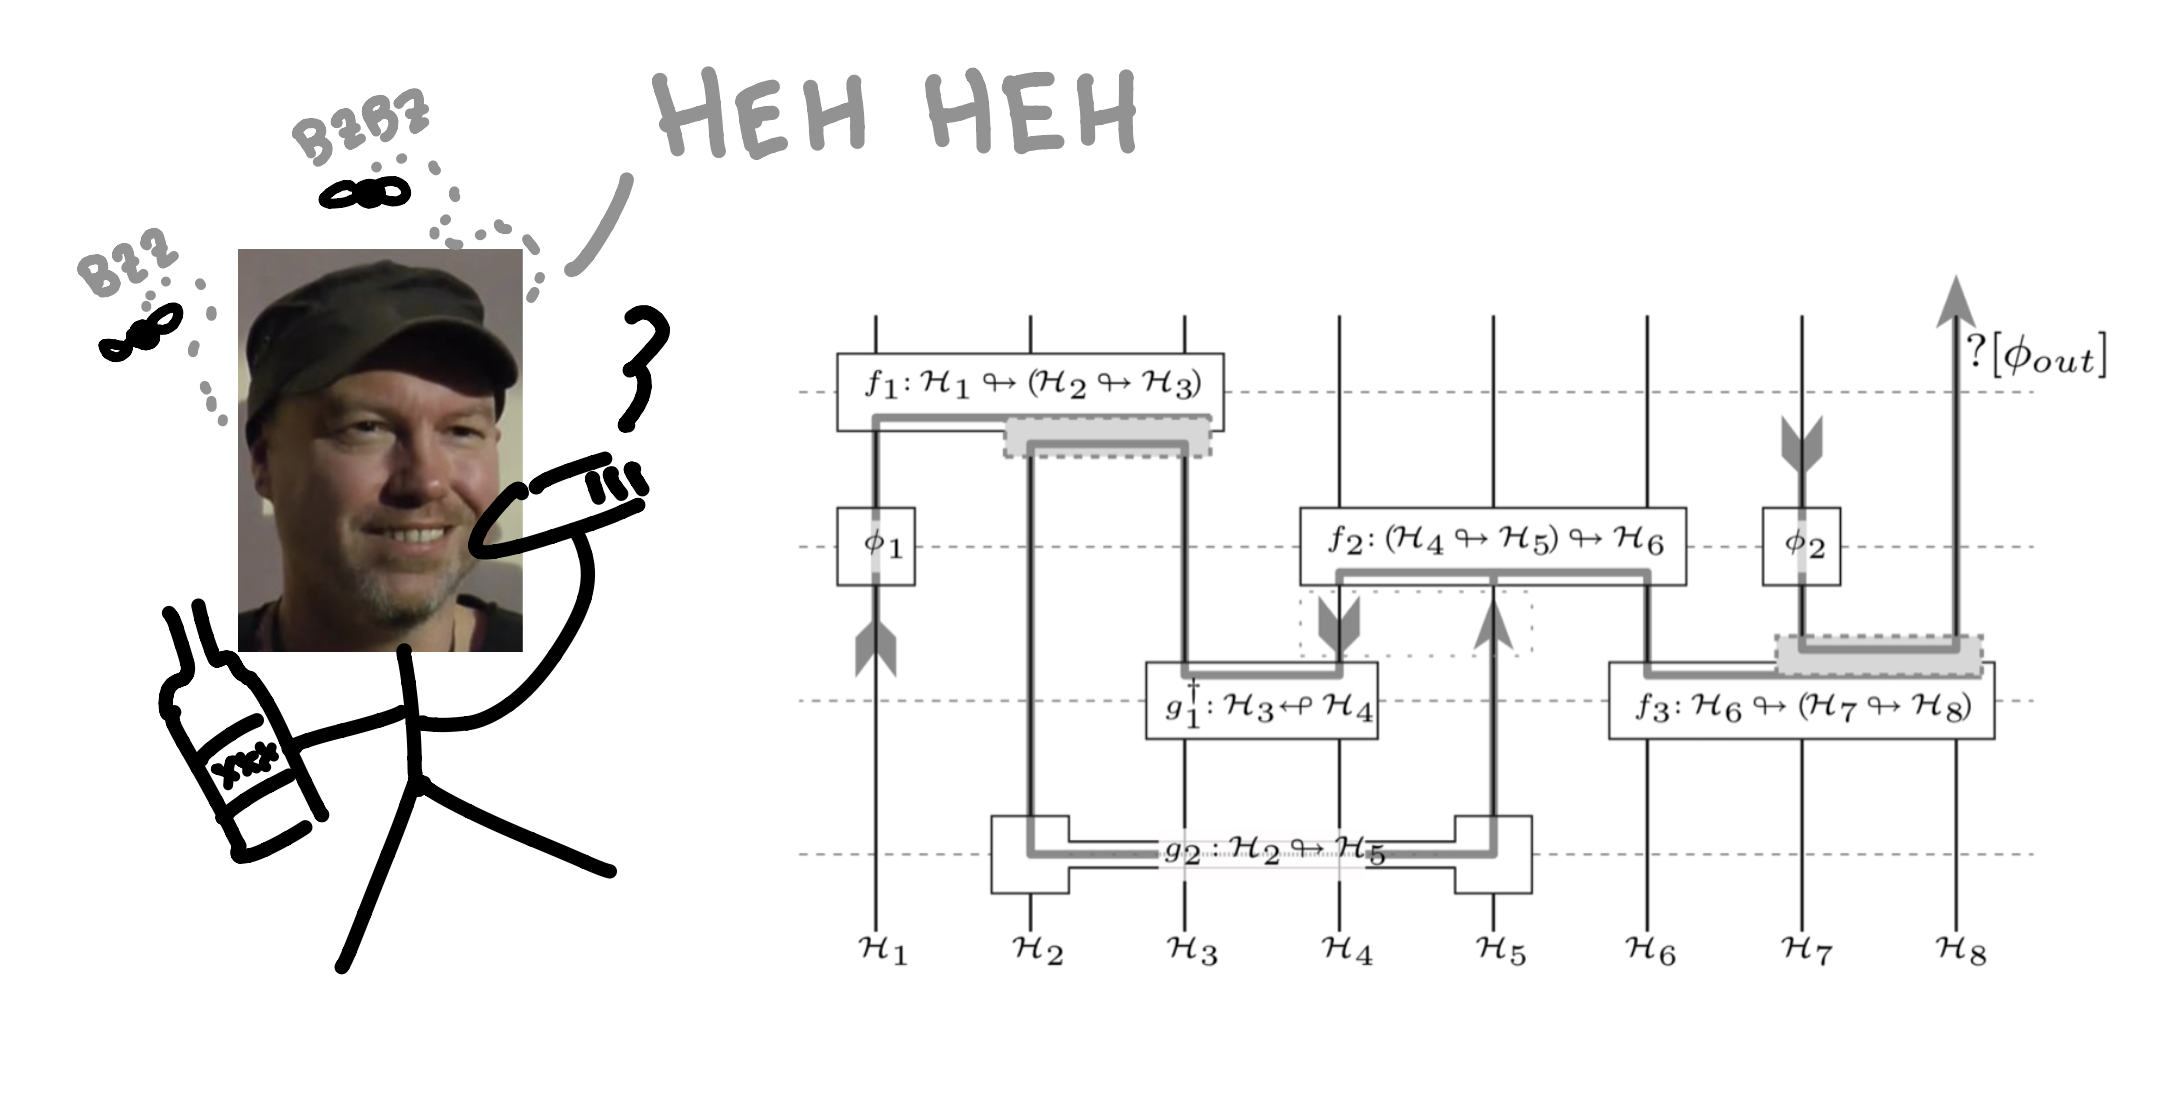
\includegraphics{figures/cartoons/bob1}}
\caption{Meanwhile, an underground grunge vagabond moonlighting as a quantum physicist moonlighting as a computer scientist was causing a shortage of cigars and whiskey in a small English town. He noticed a funny thing about the composition of multiple non-destructive measurements of a quantum system, which was that information could be carried, or flow, between them. So he wrote a paper \bR CITE \e, which contained informal diagrams that looked like this.}
\end{figure}

\begin{figure}[h!]
\centering
\scalebox{0.9}{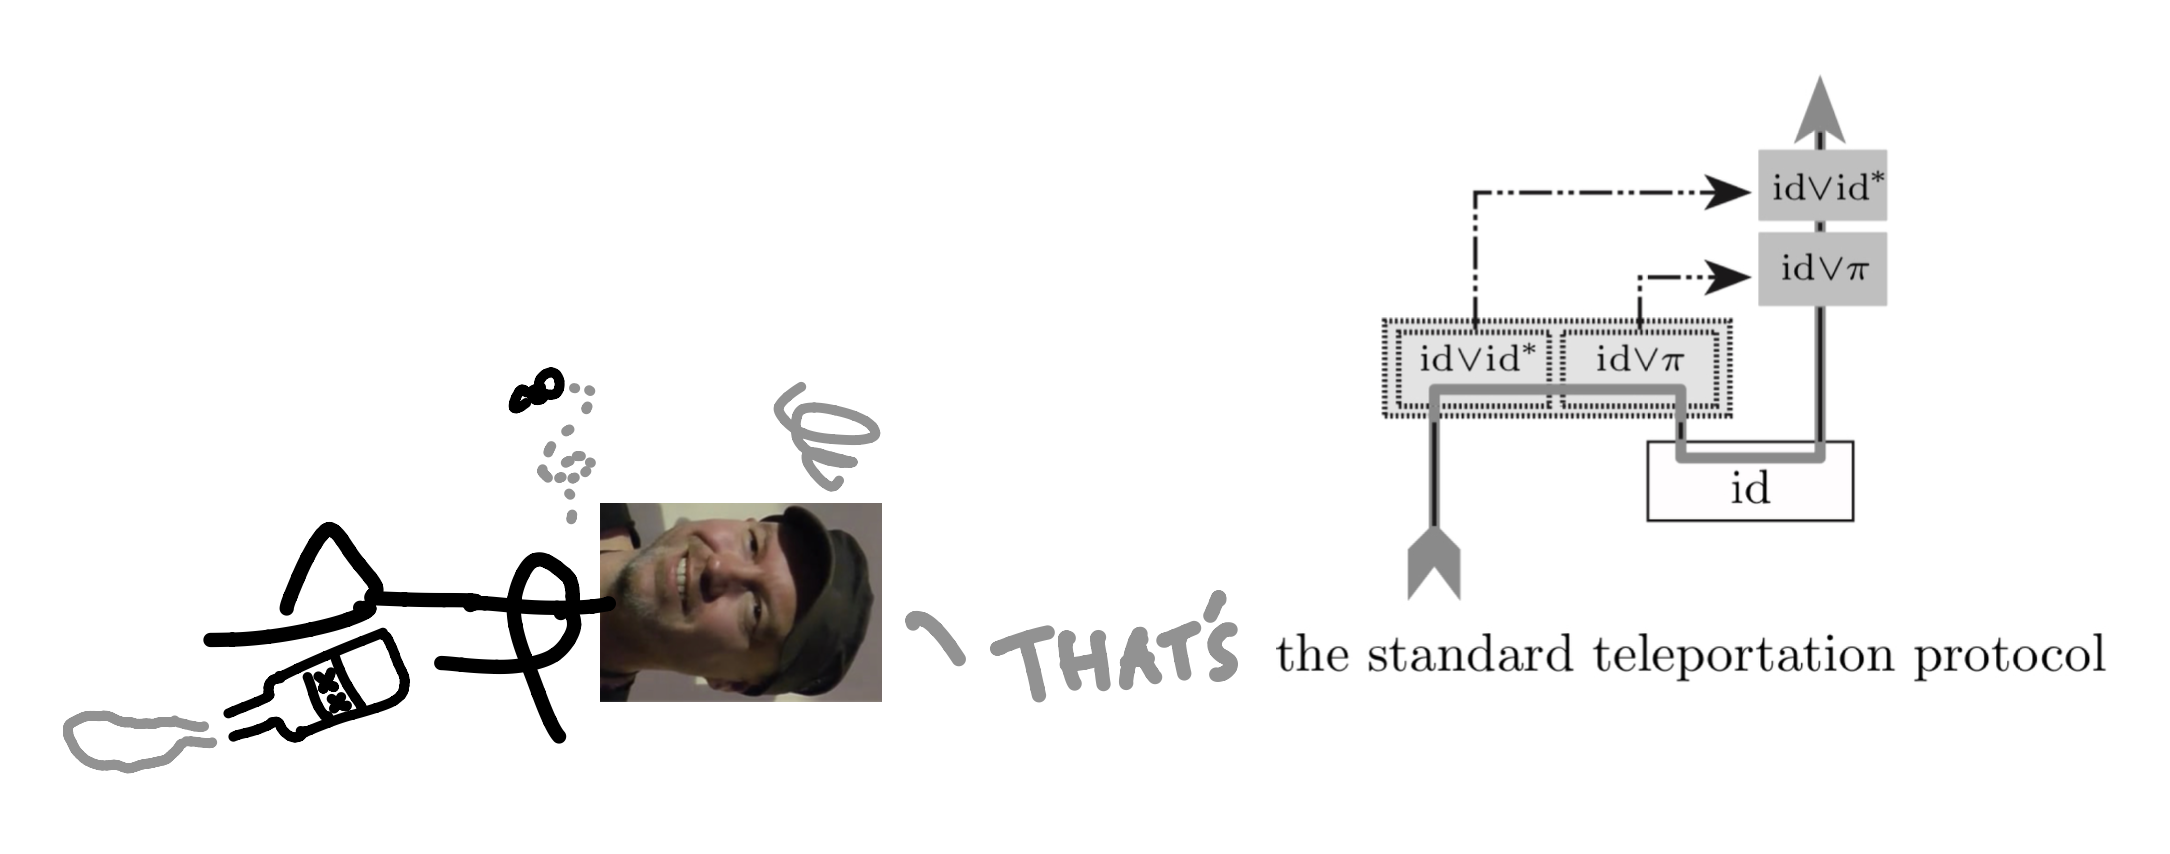
\includegraphics{figures/cartoons/bob2}}
\caption{There were two impressive things about these diagrams. First, the effects such as transparencies for text boxes and curved serifs for angled arrows give a modern feel, but they were done manually in macdraw, the diagrammatic equivalent of sticks and stones. Second, though the diagrams were informal, they provided a way to visualise and reason about entanglement that was impossible by staring at the equivalent matrix formulation of the same composite operator. The most important diagram for our story was this one, which captures the information flow of quantum teleportation.}
\end{figure}
\clearpage

\subsection{Categorical quantum mechanics}\\

\begin{figure}[h!]
\centering
\scalebox{1}{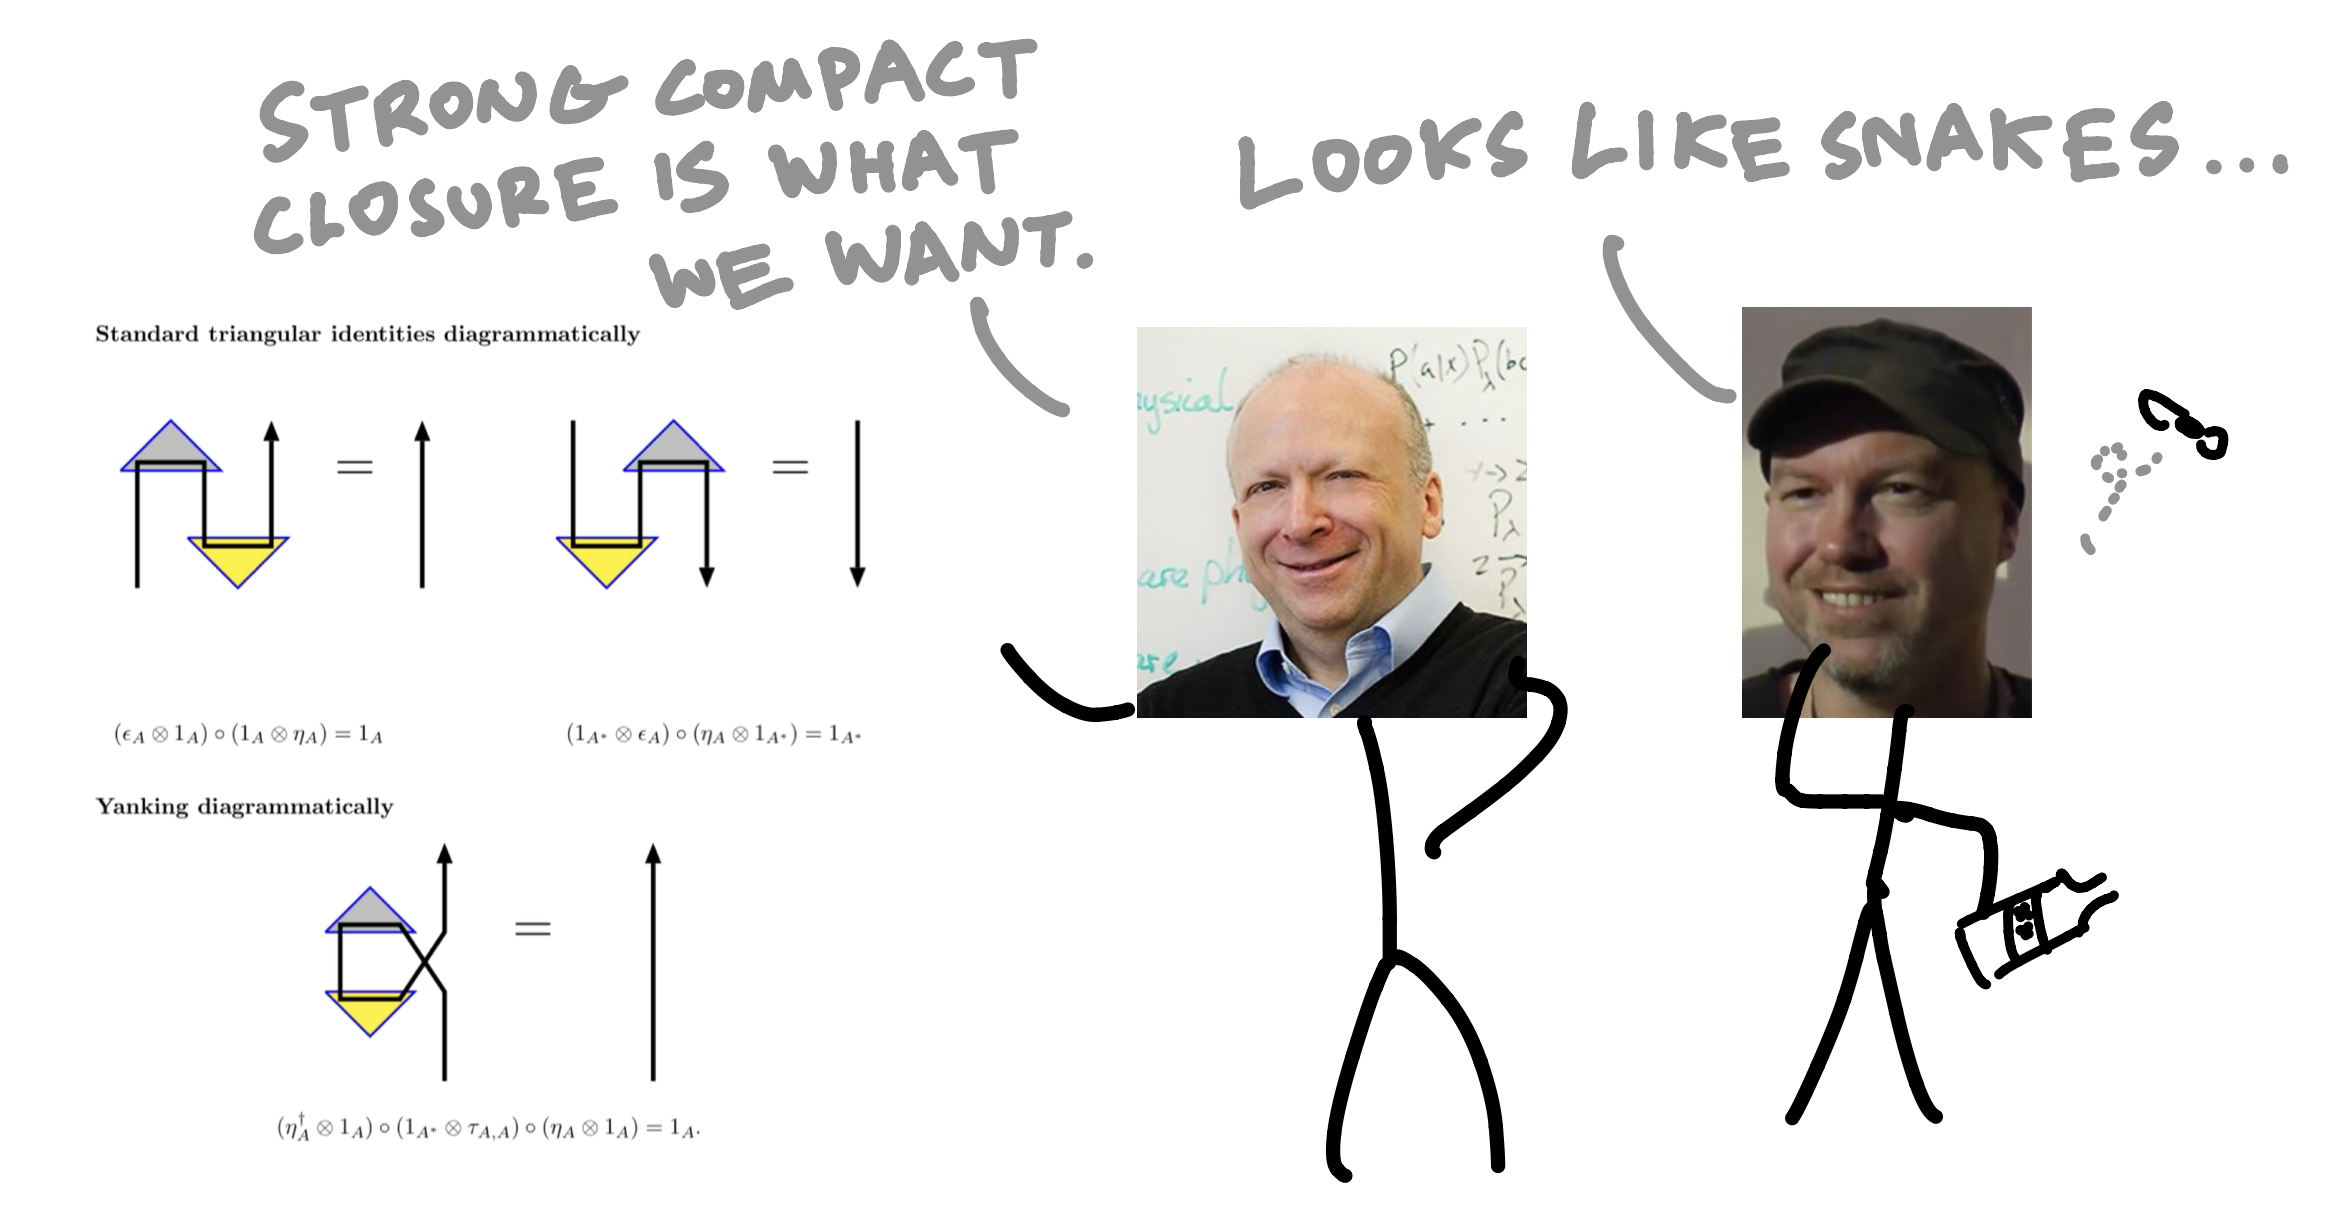
\includegraphics{figures/cartoons/samson}}
\caption{Category theorists and physicists such as Abramsky and Baez were excited about these diagrams, which looked like string diagrams waiting to be made formal. The graphical cups and caps in the important diagram were determined to correspond to a special form of symmetric monoidal closed category called strong compact closed.}
\end{figure}

\begin{figure}[h!]
\centering
\scalebox{1}{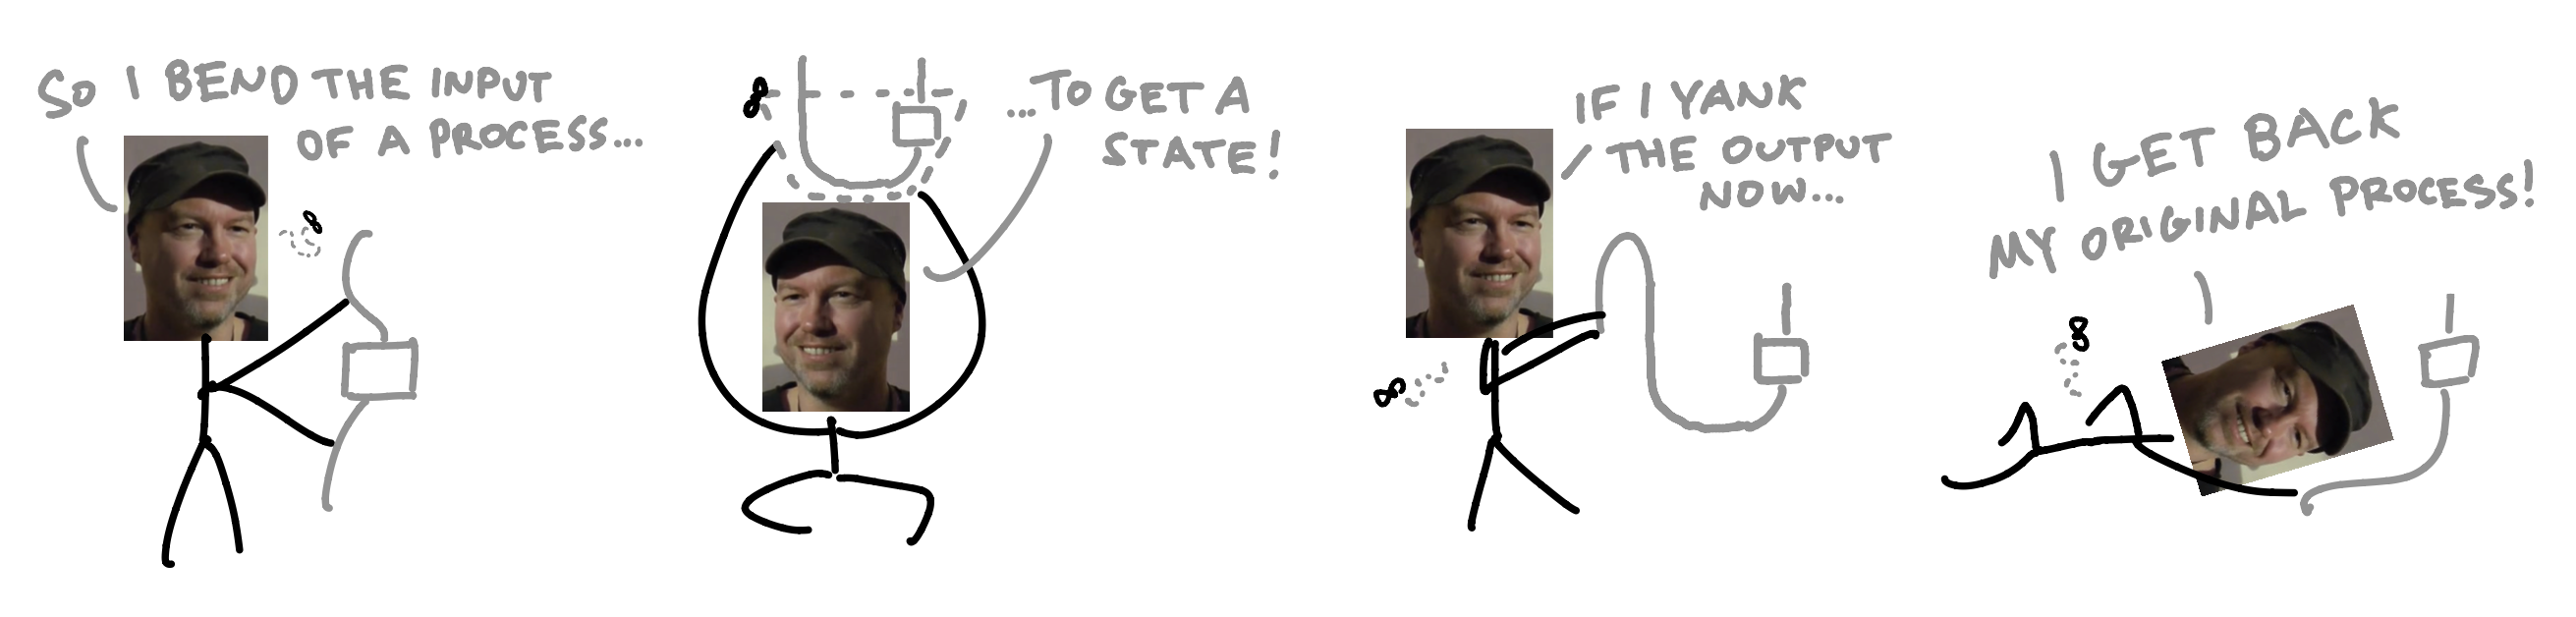
\includegraphics{figures/cartoons/cjiso}}
\caption{Diagrammatically, reasoning in a strongly compact closed category amounts to ignoring the usual requirement of processiveness and forgetting the distinction between inputs and outputs, so that "future" outputs could curl back and be "past" inputs. This formulation also gave insight into the structure of quantum mechanics. For example, the process-state duality of strong compact closure manifested as the Choi–Jamiołkowski isomorphism.}
\end{figure}

\begin{figure}[h!]
\centering
\scalebox{1}{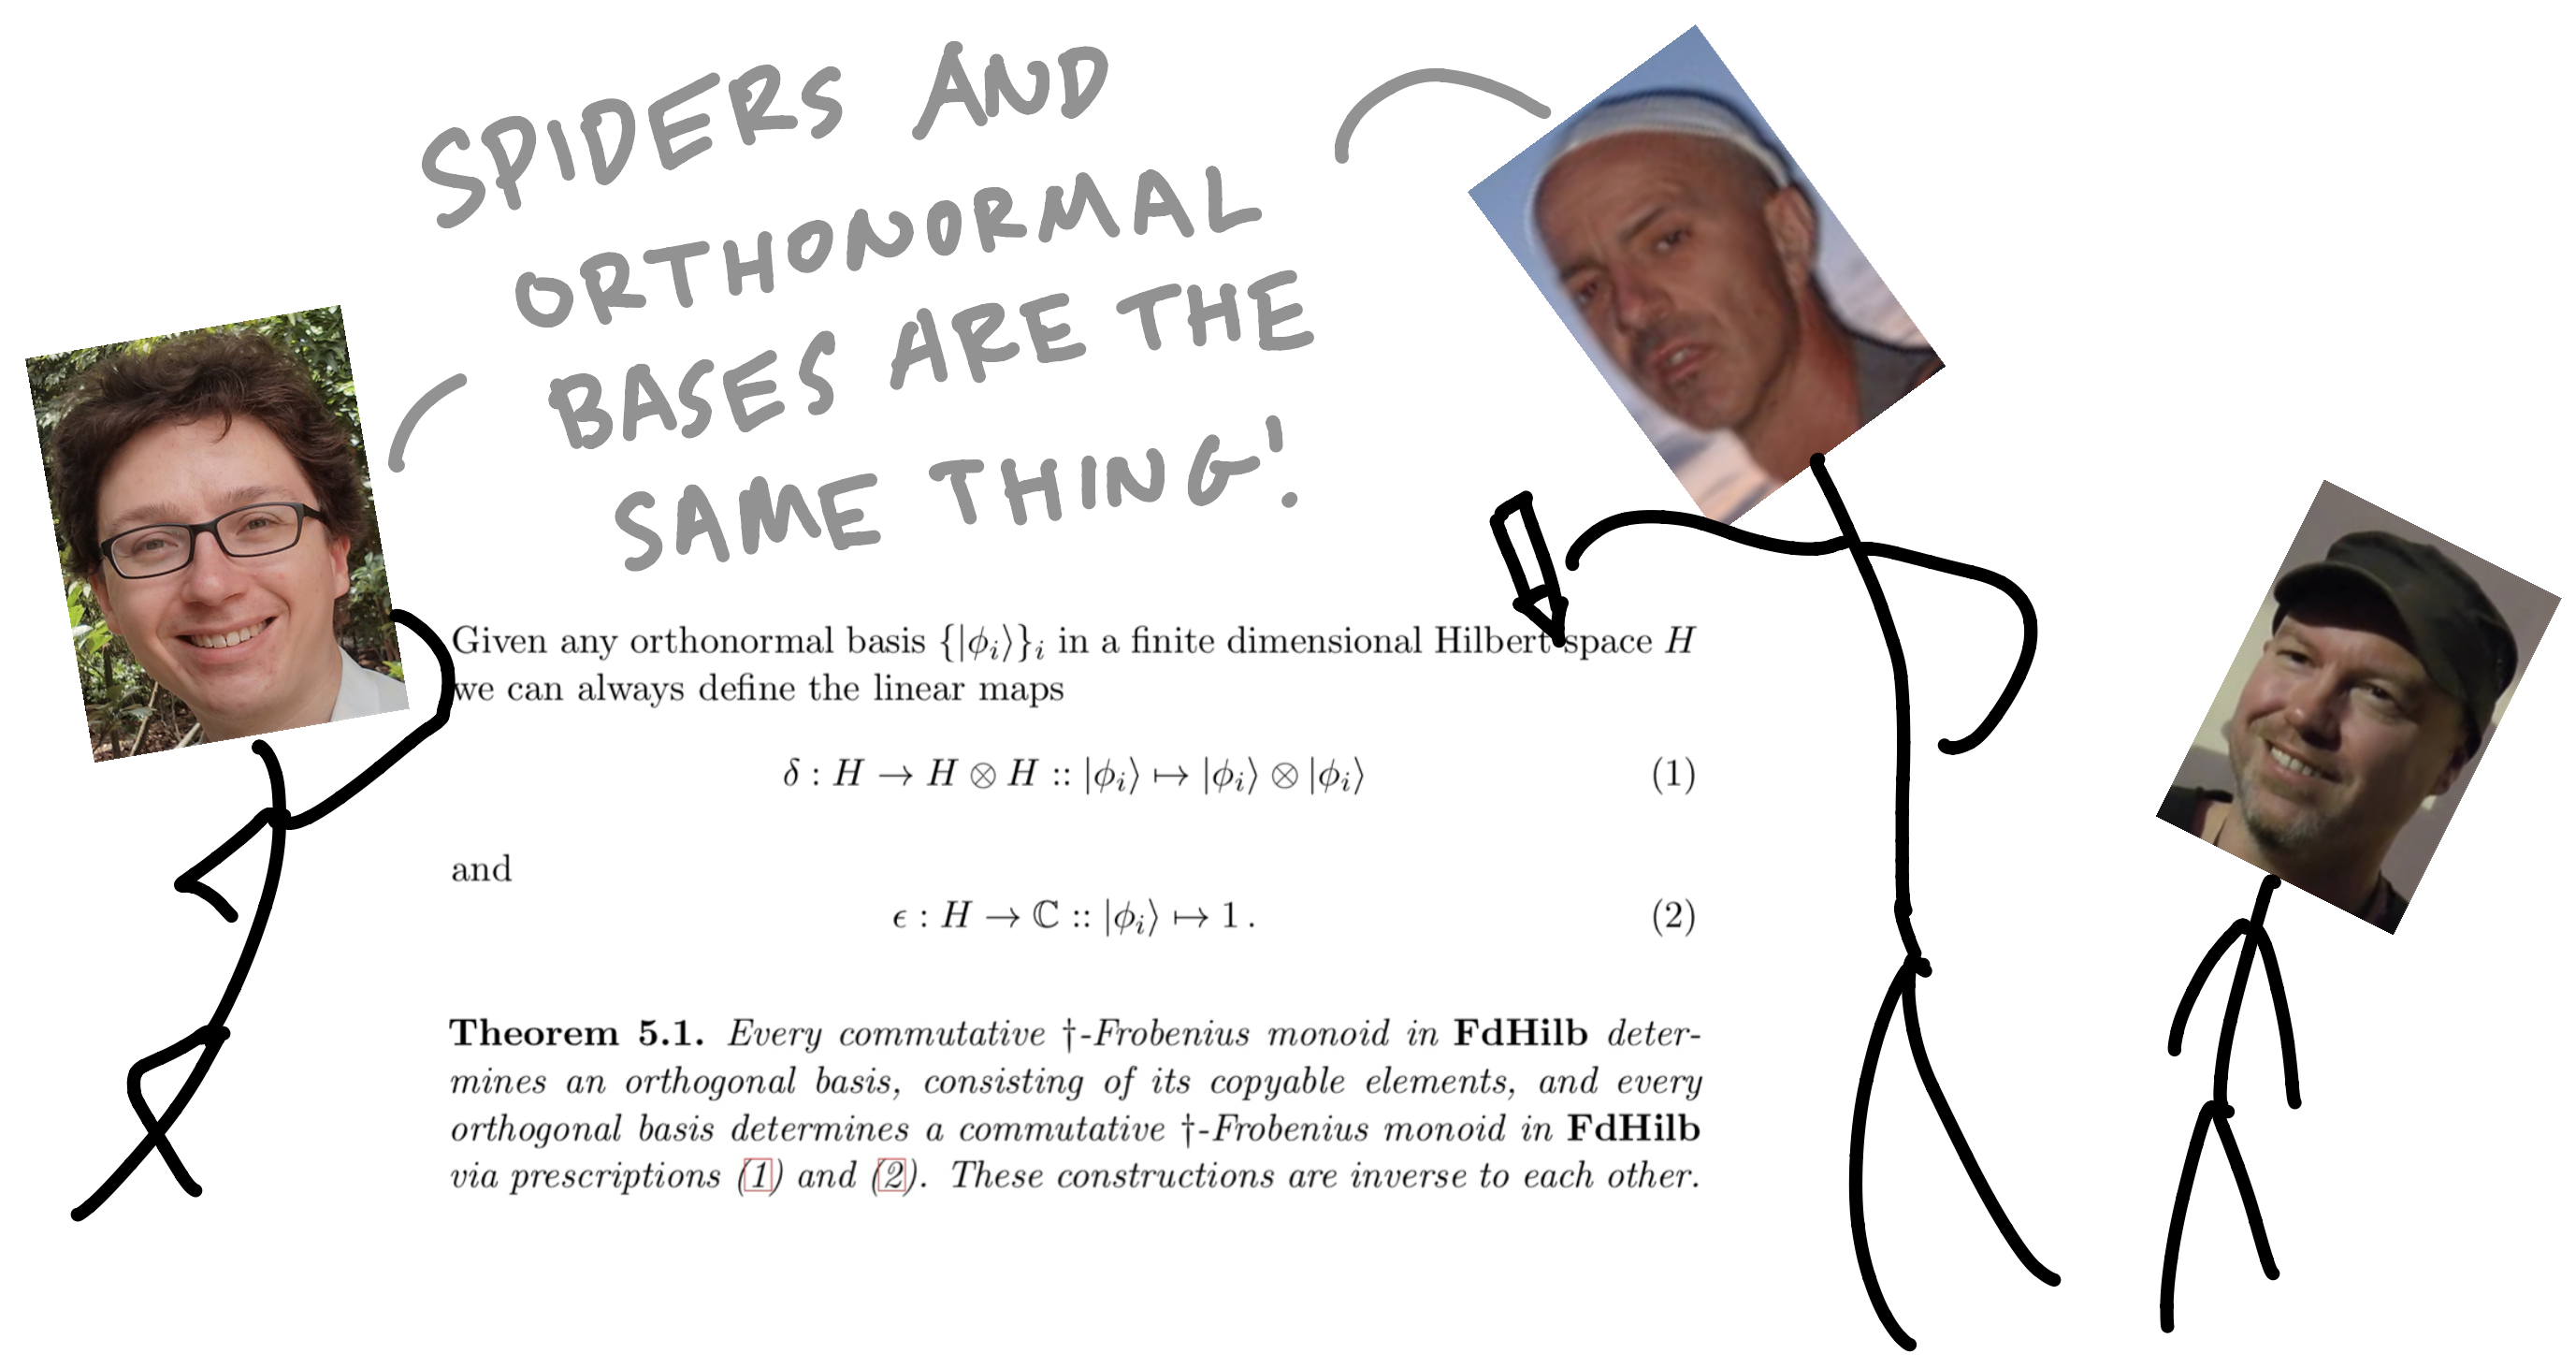
\includegraphics{figures/cartoons/spiders}}
\caption{However, dealing with superpositions necessitated using summation operators within diagrams, which is cumbersome to write especially when dealing with even theoretically simple Bell states. An elegant diagrammatic simplification arose with the observation that special-$\dagger$-frobenius algebras, or spiders, correspond to choices of orthonormal bases \bR CITE \e in \textbf{FdHilb}, the ambient setting of finite-dimensional hilbert spaces.}
\end{figure}

\begin{figure}[h!]
\centering
\[classicalquantumstructuralism\]}
\caption{Not only did this remove the need for summation operators, it also revealed that strong compact closure was a derived, rather than fundamental structure, since spiders induce compact closed structure.}
\end{figure}

\begin{figure}[h!]
\centering
\scalebox{1}{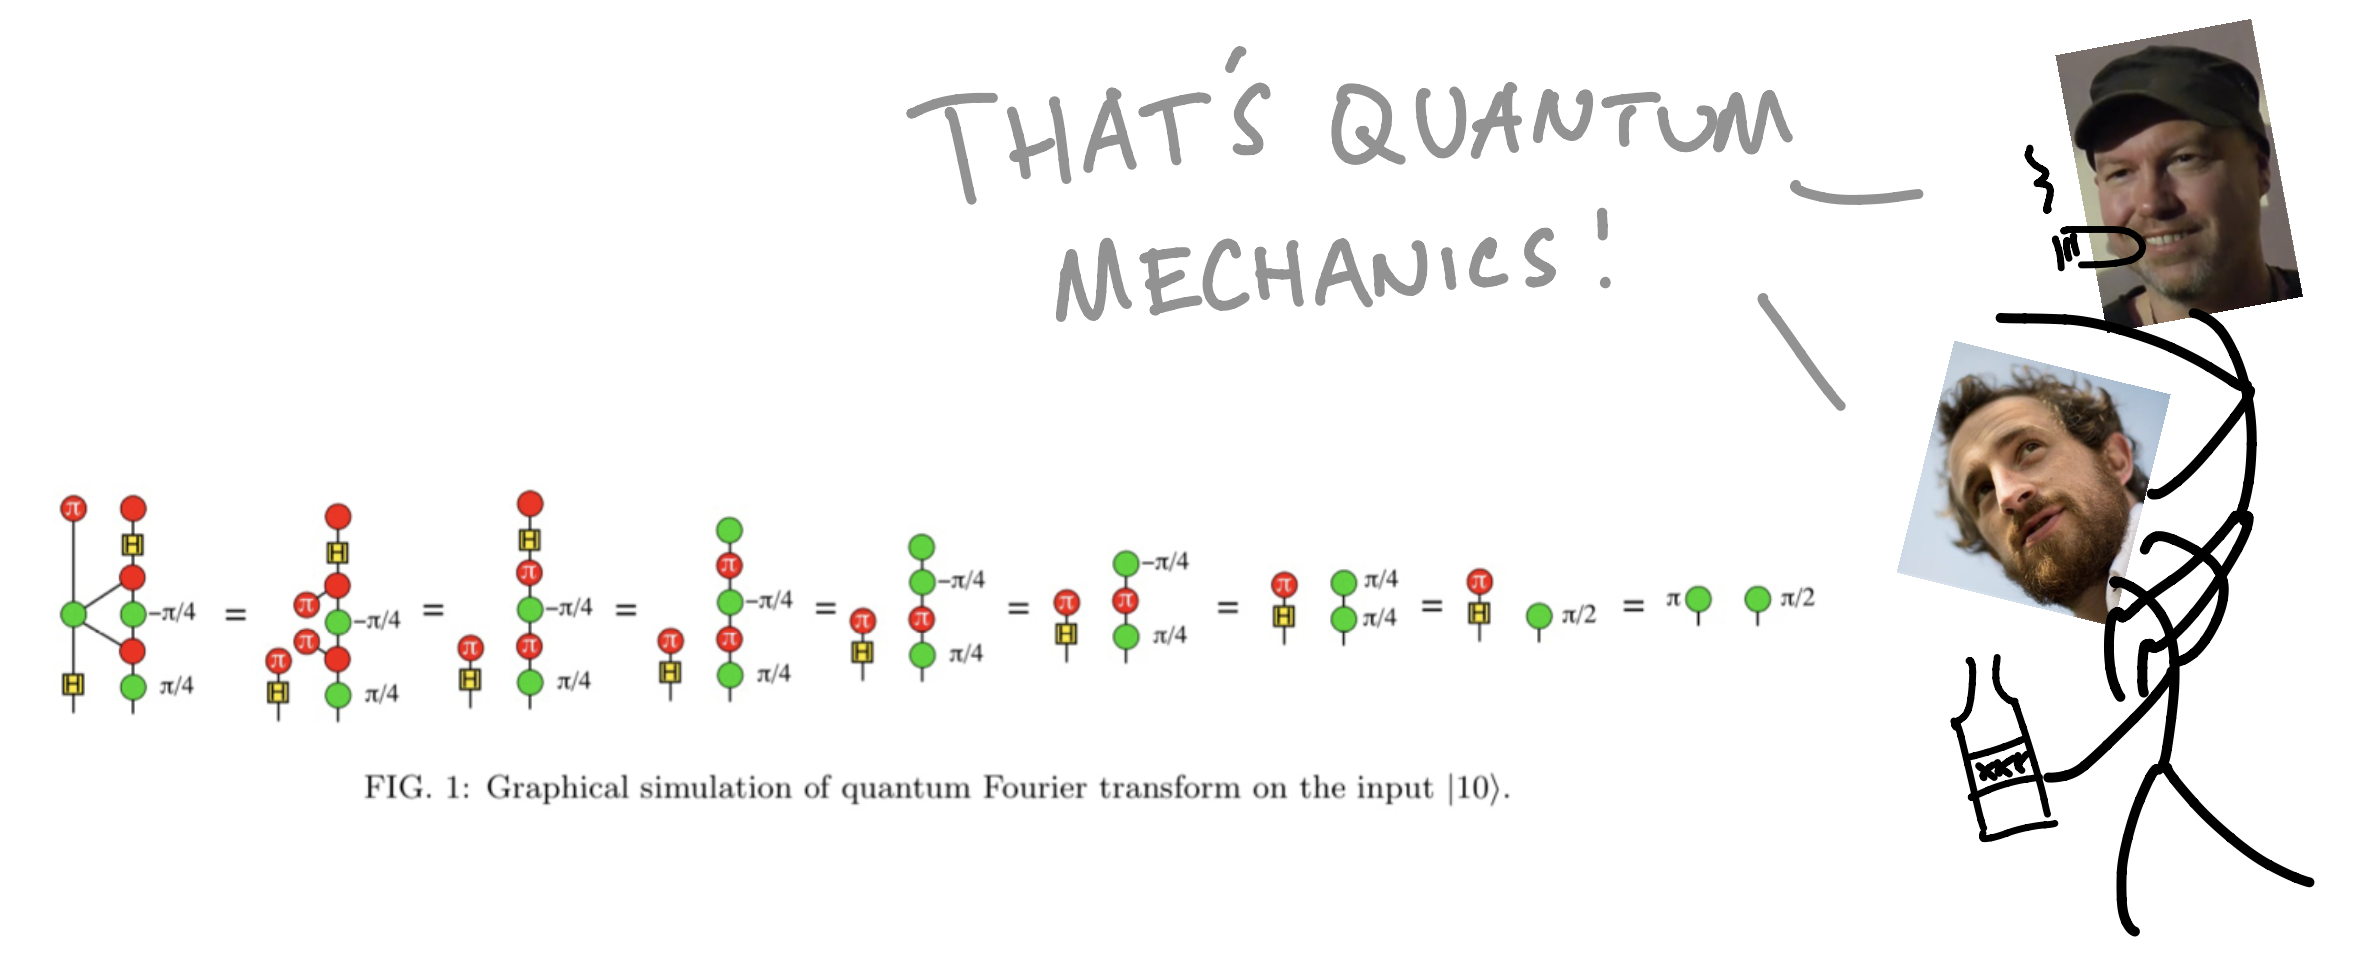
\includegraphics{figures/cartoons/ross}}
\caption{And so the stage was set for a purely diagrammatic treatment of ZX quantum mechanics. The story of ZX diverges away from our interest, so I will summarise what happened afterwards. In no particular order, the development of ZX went on to accommodate a third axis of measurement to yield a ZXW calculus \bR CITE \e, the systems were proven to be complete \bR CITES \e, there are at the time of writing two expository books \bR CITES \e, and ZX-variants are becoming an industry standard for quantum circuit specification and rewriting \bR CITE \e.}
\end{figure}
\clearpage

\subsection{Enter computational linguistics}

\begin{figure}[h!]
\centering
\scalebox{1}{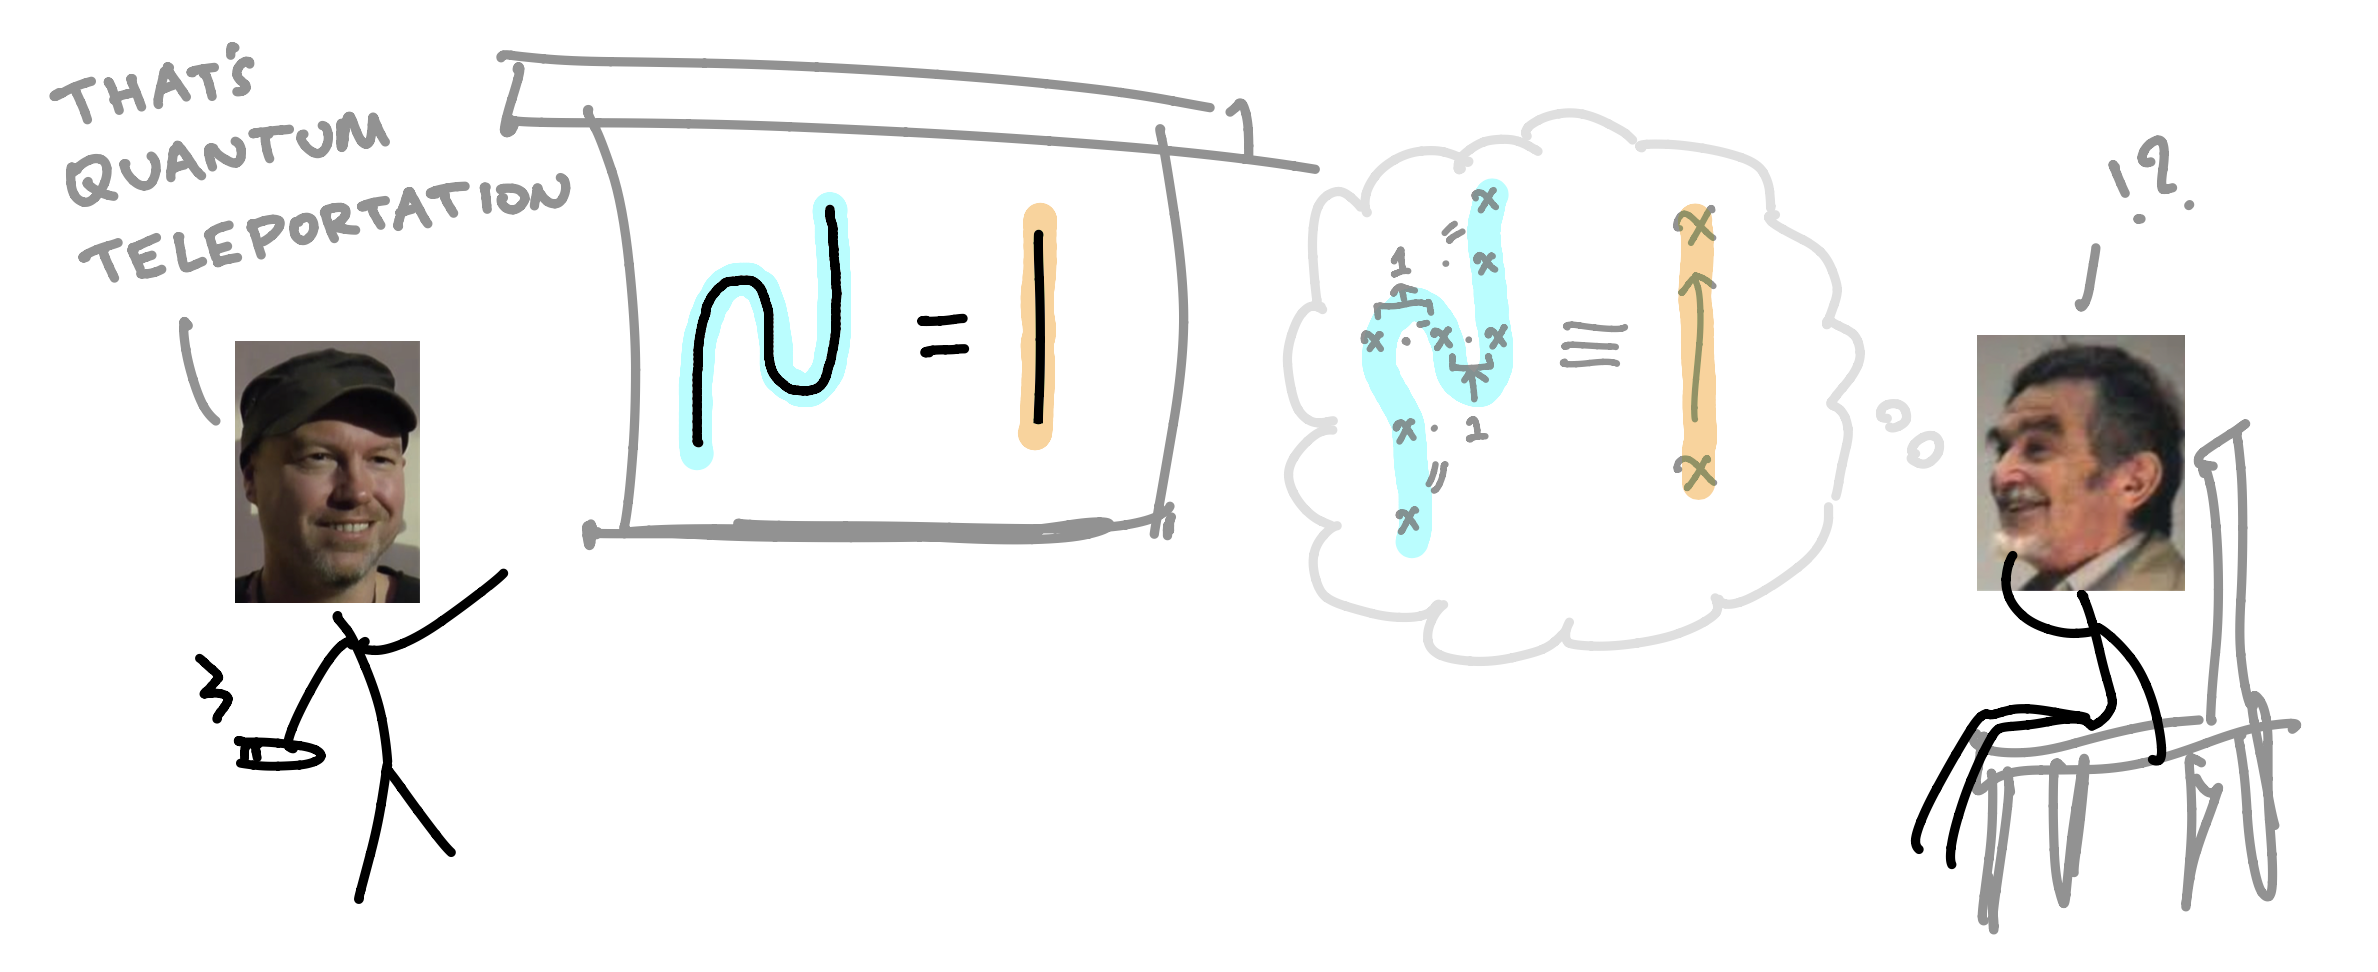
\includegraphics{figures/cartoons/boblambek1}}
\caption{Somewhere in Canada at the turn of the millenium, Bob met Jim, who saw something familiar about the diagram for quantum teleportation. The snake equation for compact closure looked a lot like the categorified version of introducing and eliminating pregroup types.
}
\end{figure}

\begin{figure}[h!]
\centering
\scalebox{1}{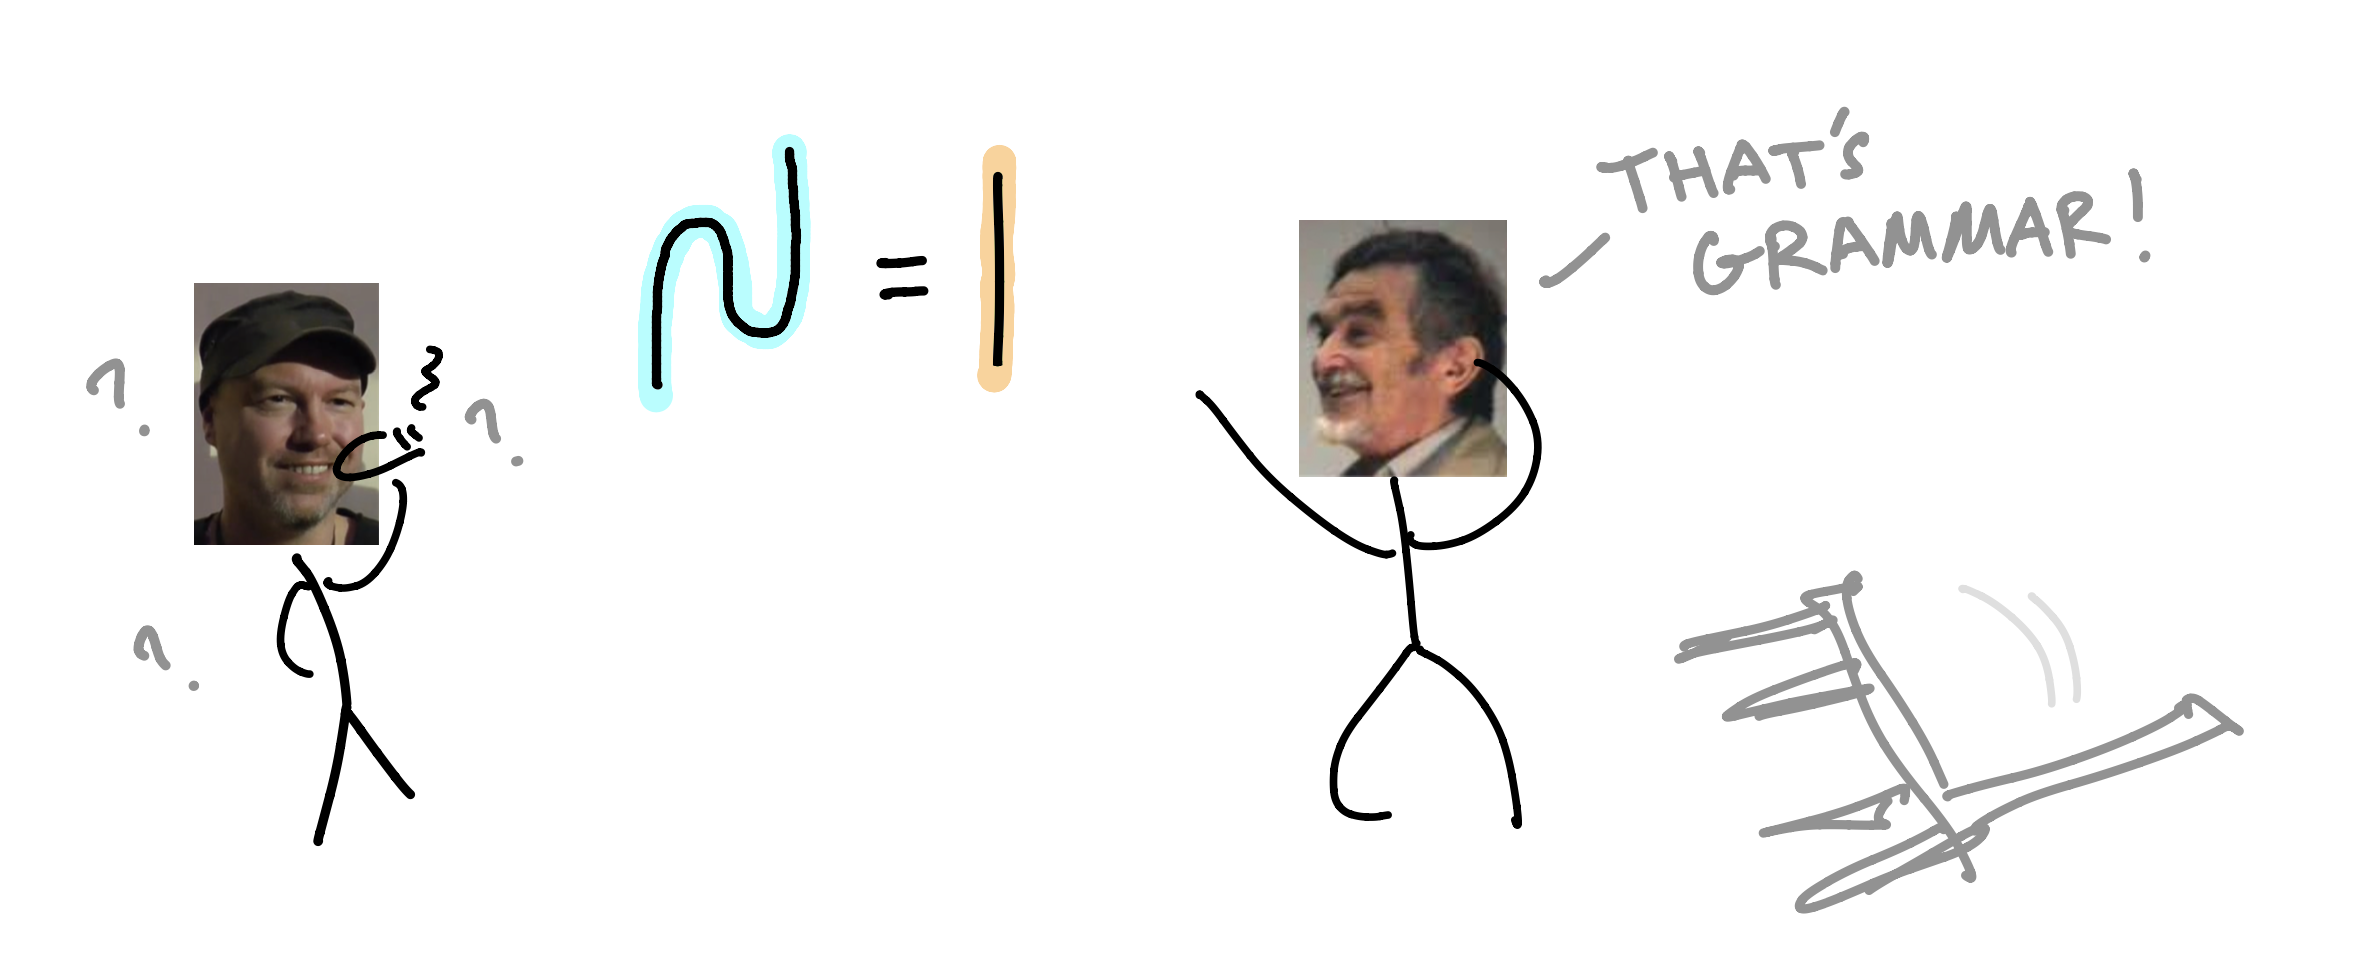
\includegraphics{figures/cartoons/boblambek2}}
\caption{Bob and Jim's meeting put the adjectives \emph{compositional} and \emph{categorical} on the same table, but the cake wasn't ready. Two more actors Steve and Mehrnoosh were required to introduce \emph{distributional}, which refers to Firth's maxim \bR CITE \e "you shall know a word by the company it keeps". In its modern incarnation, this refers generally to vector-based semantics for words, where it is desirable but not necessarily so (as in the case of generic latent space embeddings by an autoencoder) that proximity of vectors models semantic closeness.}
\end{figure}

\begin{figure}[h!]
\centering
\scalebox{1}{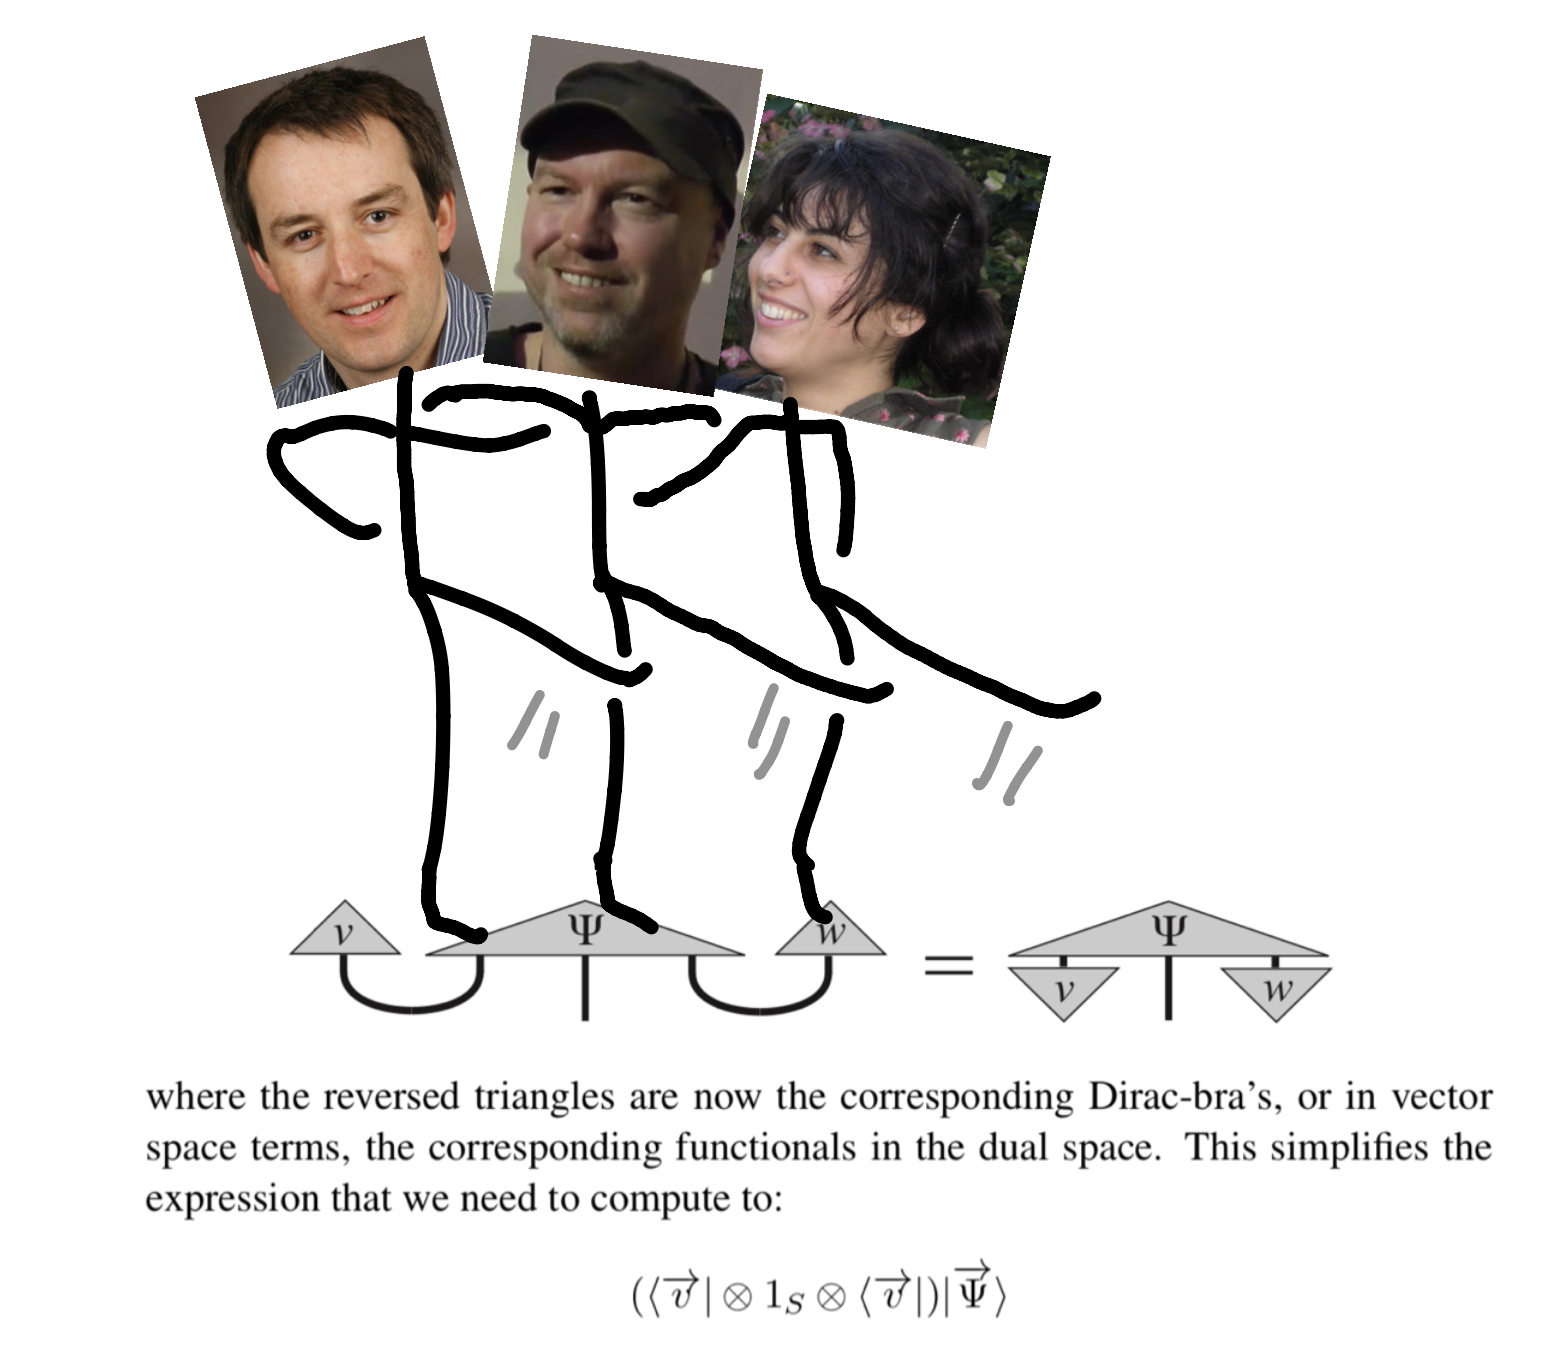
\includegraphics{figures/cartoons/disco1}}
\caption{Steve Clark was a professor in the computer science department at Oxford, and he was wondering how to compose vector-based semantic representations. Steve asked Bob, who realised suddenly what Jim was talking about. Mediated by the linguistic expertise of Mehrnoosh who was a postdoctoral researcher in Oxford at the time, pregroup diagrams were born. The basic types $n$ and $s$ are assigned finite-dimensional vector spaces, concatenation of types the kronecker product $\otimes$, and by the isomorphism of dual spaces in finite dimensions there is no need to keep track of the left- and right- inverse data. Words become vectors, and pregroup reductions become bell-states, or bell-measurements, depending on whether one reads top-down or bottom-up. There was simply no other game in town for an approach to computational linguistics that combined linguistic compositionality with distributional representations.}
\end{figure}

\begin{figure}[h!]
\centering
\scalebox{1}{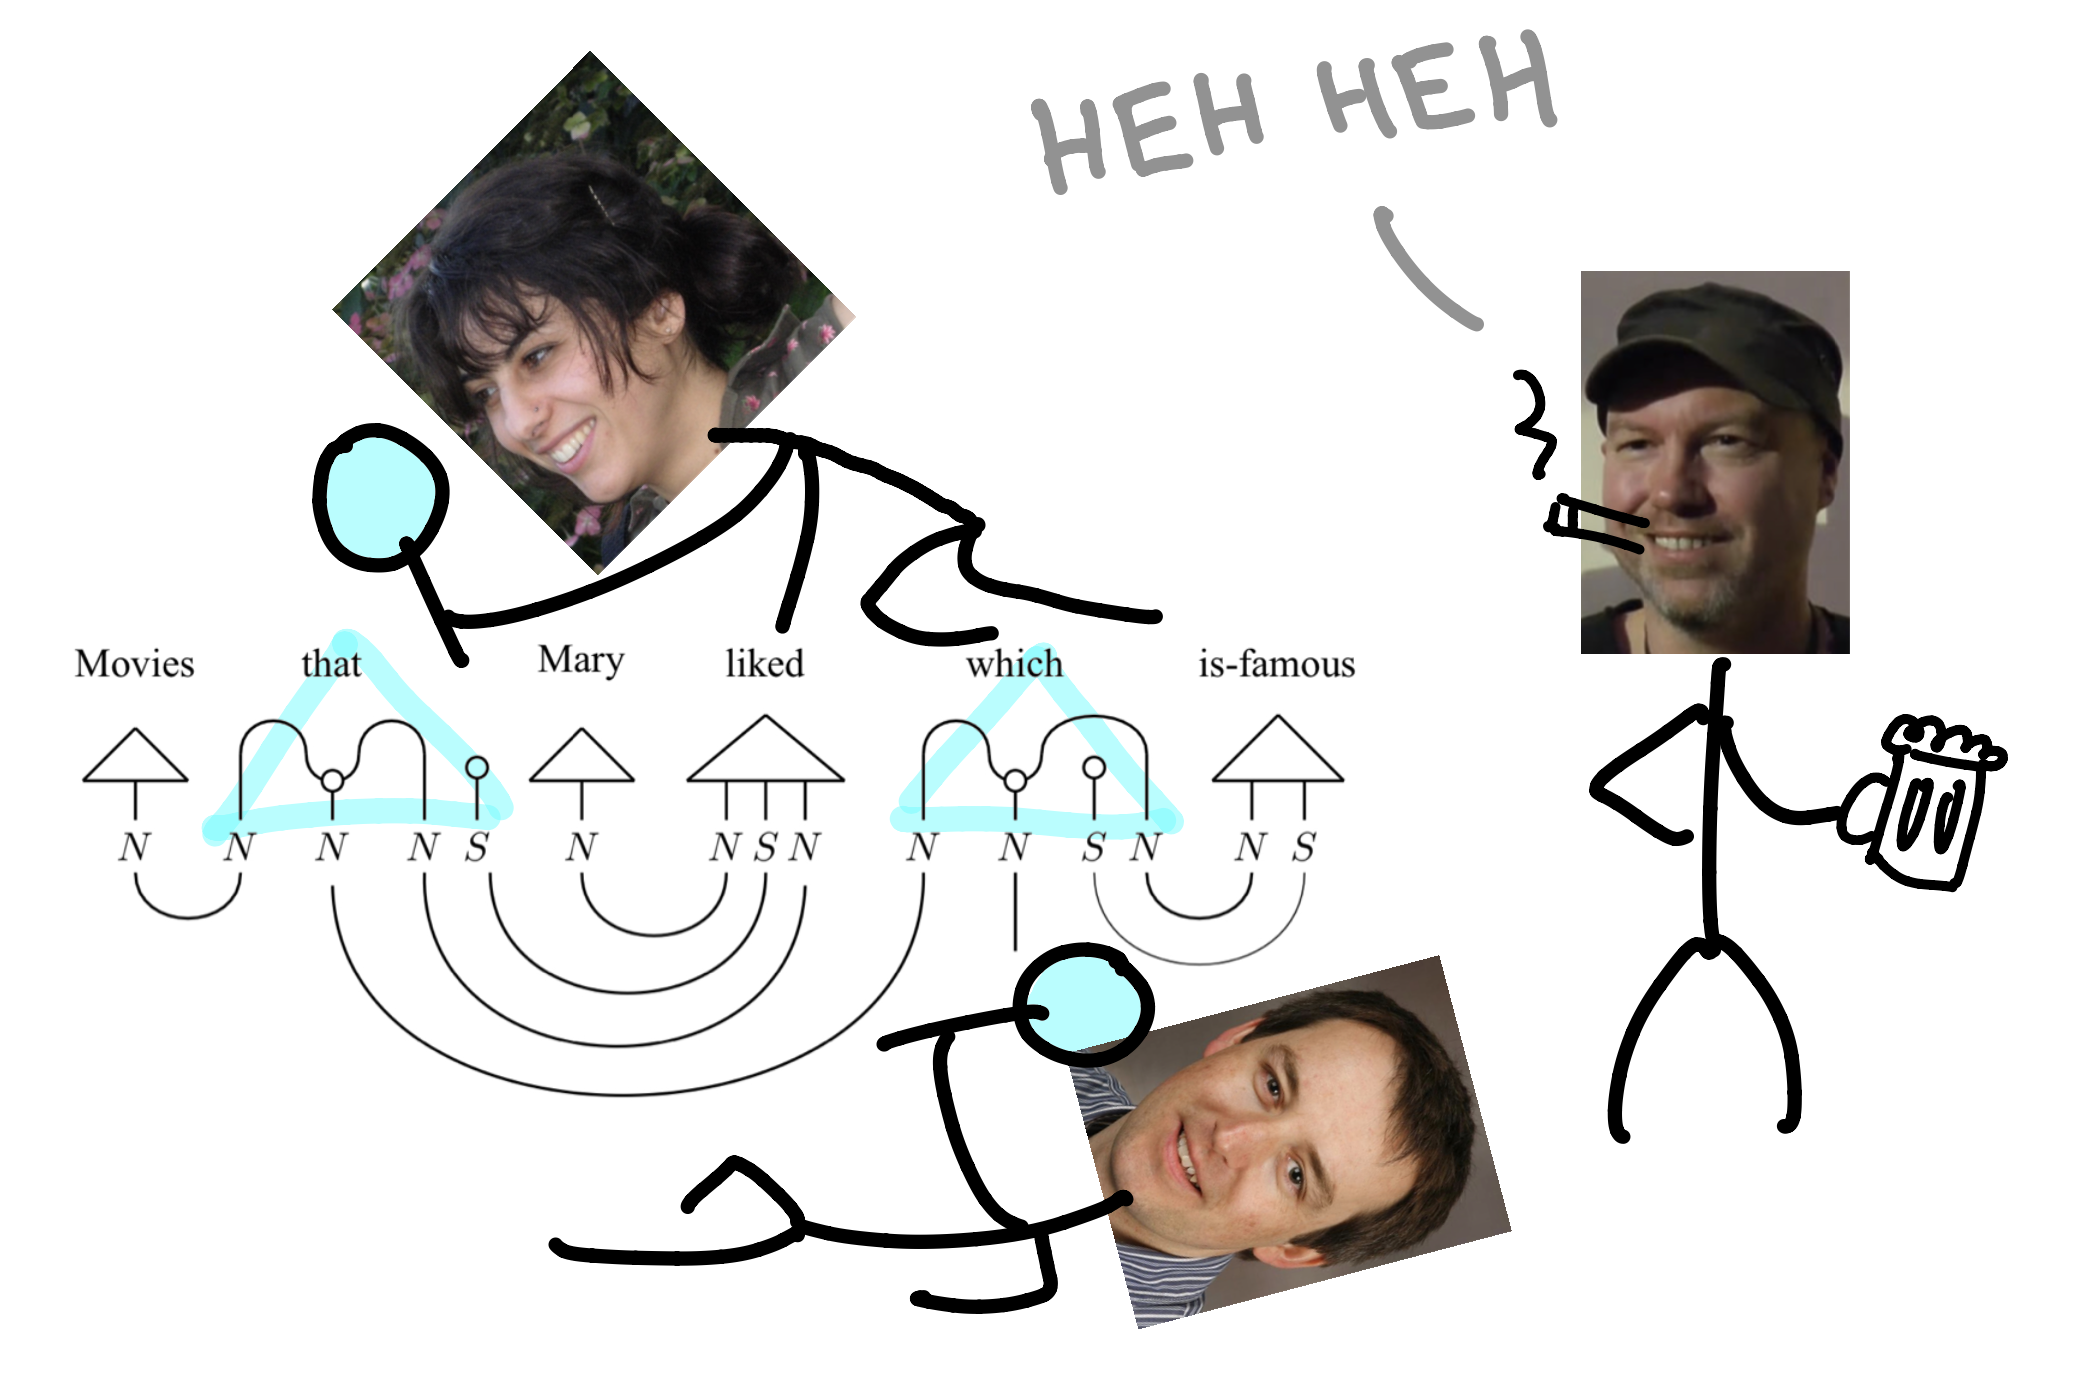
\includegraphics{figures/cartoons/disco2}}
\caption{In \emph{the frobenius anatomy of relative pronouns}\bR CITE \e, the trio realised that spiders could play the role of relative pronouns, which was genuinely novel linguistics. If one follows the noun-wire of "movies", one sees that by declaring the relative pronoun to be a vector made up of a particular bunch of spiders-as-multiwires, "movies" is copied to be related to the "liked" word, copied again by "which" to be related to the "is-famous" word, and a third time to act as the noun in the whole noun-phrase. This discovery clarified a value proposition: insights from quantum theory could be applied in the linguistic setting, and linguistics offered a novel use-case for quantum computers. For example, density matrices were used to model semantic ambiguity \bR CITE \e, and natural language experiments were performed on real quantum computeres \bR CITE \e.}
\end{figure}

\begin{figure}[h!]
\centering
\scalebox{1}{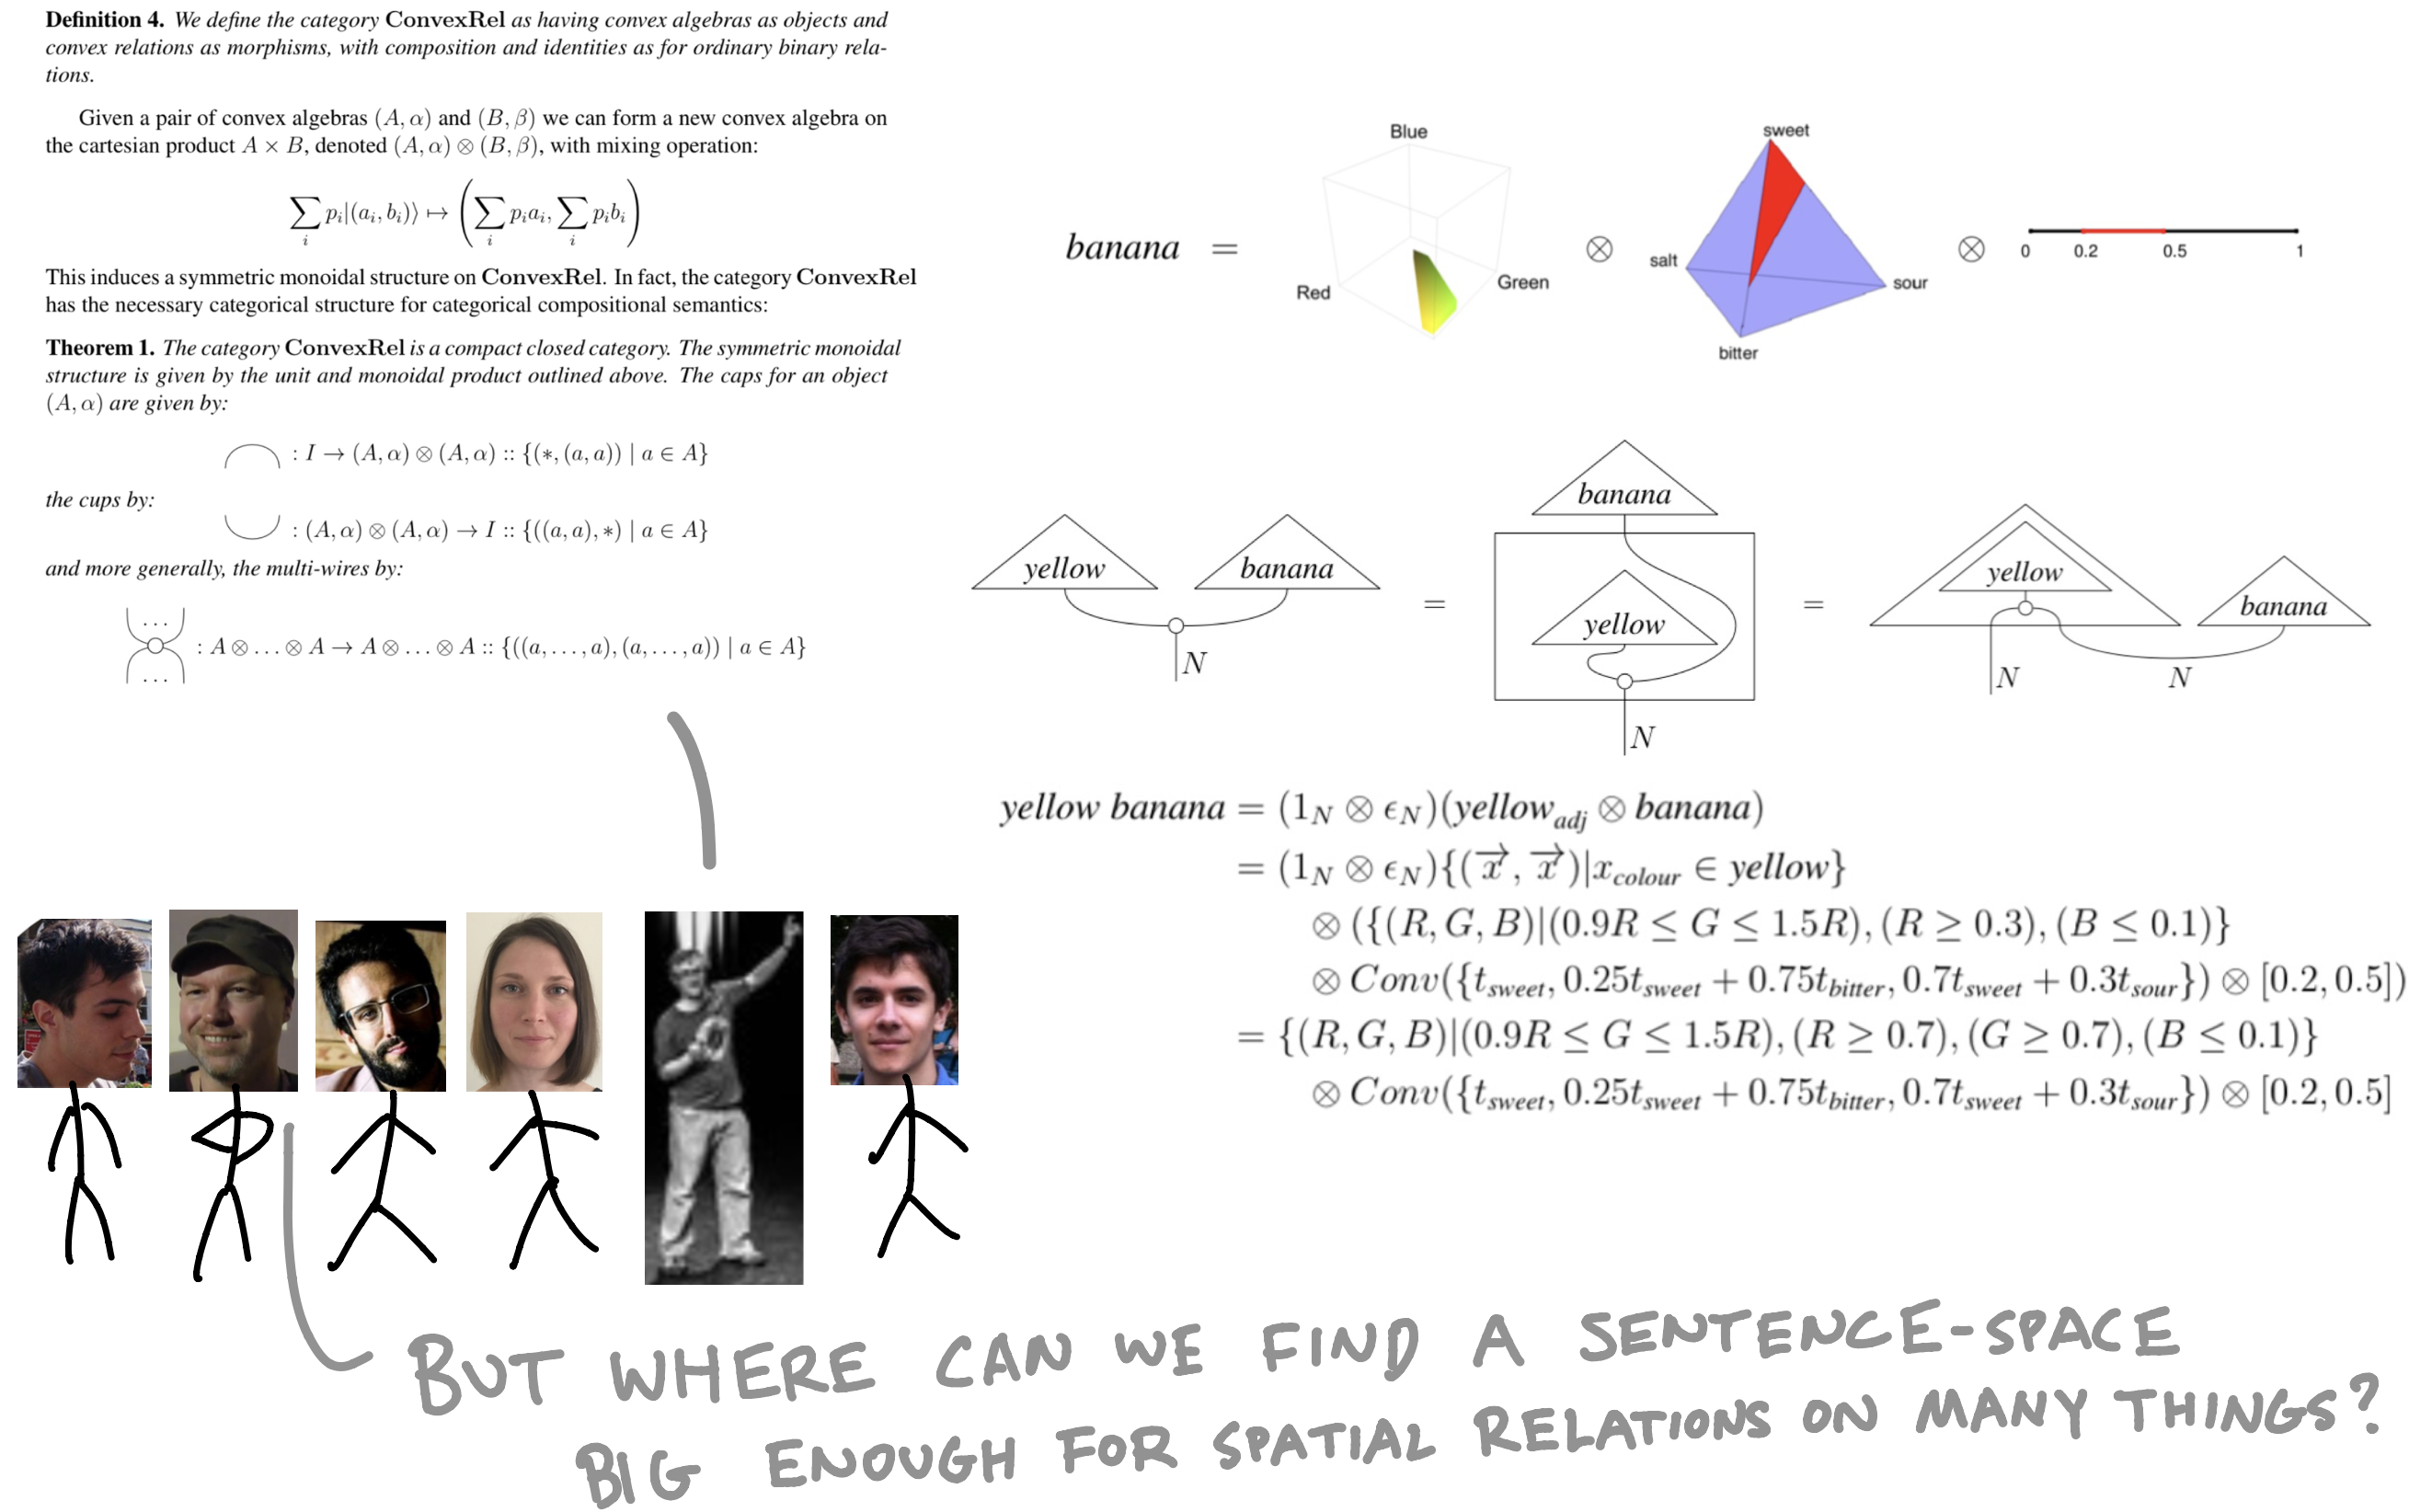
\includegraphics{figures/cartoons/disco3}}
\caption{Keeping the structure of the diagrams but seeking set-relational rather than vector-based semantics, a bridge was made between linguistics and cognitive science in \emph{interacting conceptual spaces I}\bR CITE \e. Briefly, G\"{a}rdenfors posits that spatial representations of concepts mediate raw sense data and symbolic representations -- e.g. red is a region in colourspace -- and moreover that concepts ought to be spatially convex -- e.g. mixing any two shades of red still gives red. This paper created a new point in the value proposition: that new mathematics would arise from investigating the linguistic-quantum bridge, e.g. generalised relations \bR CITE \e. Although labelled as if it is the first in a series, the paper never saw a sequel by the same title, blocked by an apparently simple but actually tricky theoretical problem. The problem is that while this convex-relational story worked for conceptual adjectives modifying a single noun such for "sweet yellow bananas", there was difficulty in extending the story to work for multiple objects interacting in the same space, as in "cup on table in room". It couldn't be worked out what structure a sentence-wire in \textbf{ConvexRel} ought to have in order to accommodate (in principle) arbitrarily many objects and spatial relations between them.\\

DisCoCat then diverges from the story I want to tell. In no particular order, QNLP was done on an actual quantum computer \bR CITE \e, some software packages were written \bR CITE \e, and some art was made \bR CITE \e.}
\end{figure}
\clearpage



\subsection{I killed DisCoCat, and I would do it again.}

\begin{figure}[h!]
\centering
\scalebox{1}{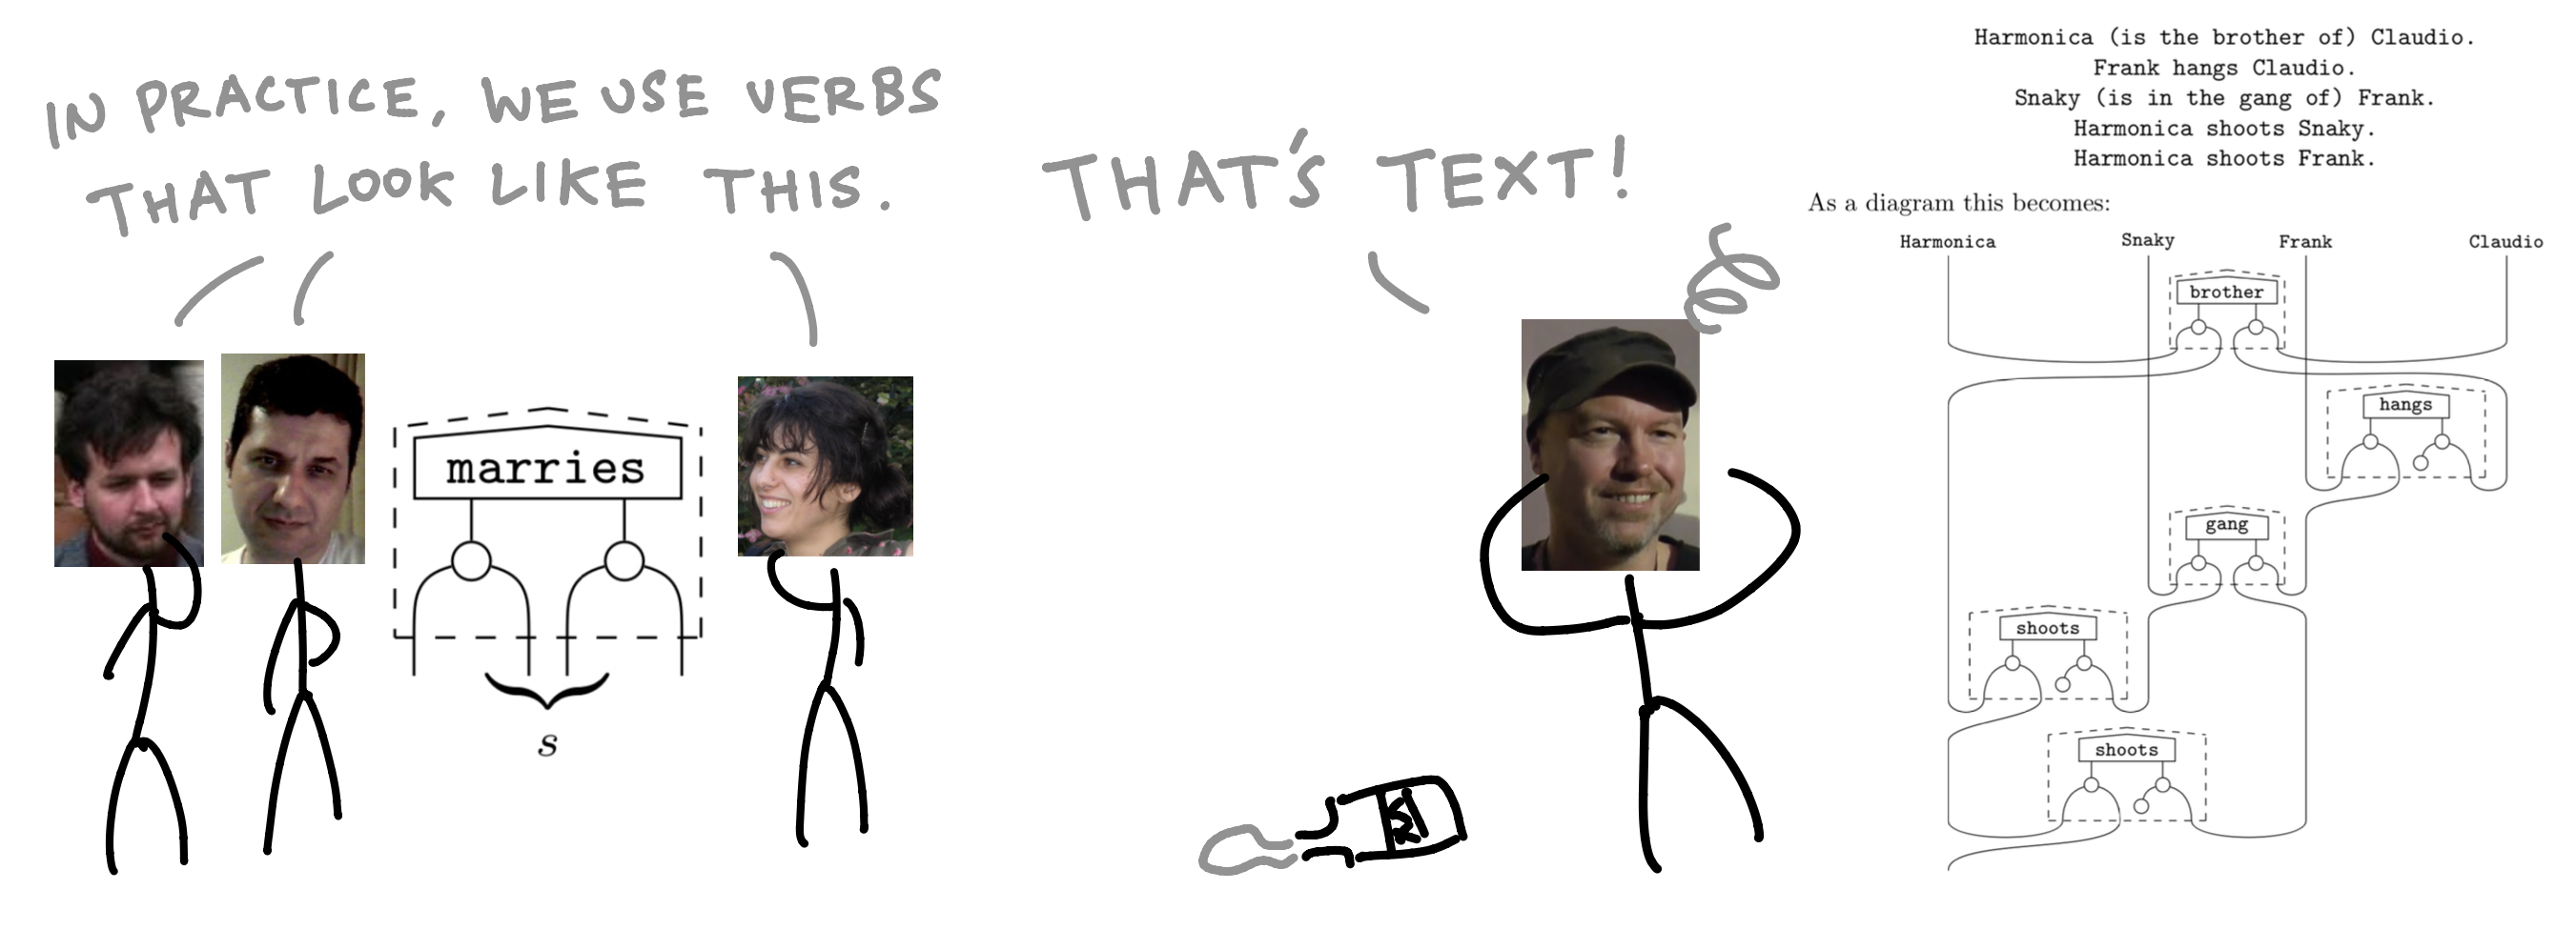
\includegraphics{figures/cartoons/discocirc1}}
\caption{It is a common evolutionary step in linguistics that theories `break the sentential barrier', moving from sentence-restricted to text- or discourse-level analysis \bR CITE \e. The same thing happened with DisCoCirc, due to a combination of practical constraints and theoretical ambition. On the practical side, wide tensors were (and remain) prohibitively expensive to simulate classically and actual quantum computers did not (and still do not) have many qubits, hence in practice pregroup diagrams were reduced to thinner and deeper circuits, often with the help of an additional simplifying assumption that sentence wires were pairs of noun wires in the illustrated form on the left. Theoretically, seeking dynamic epistemic logic, Bob had an epiphanous hangover (really) where he envisioned that these "Cartesian verbs" could be used in service of compositional text meanings, and he called this idea DisCoCirc \bR CITE \e.}
\end{figure}

\begin{figure}[h!]
\centering
\scalebox{1}{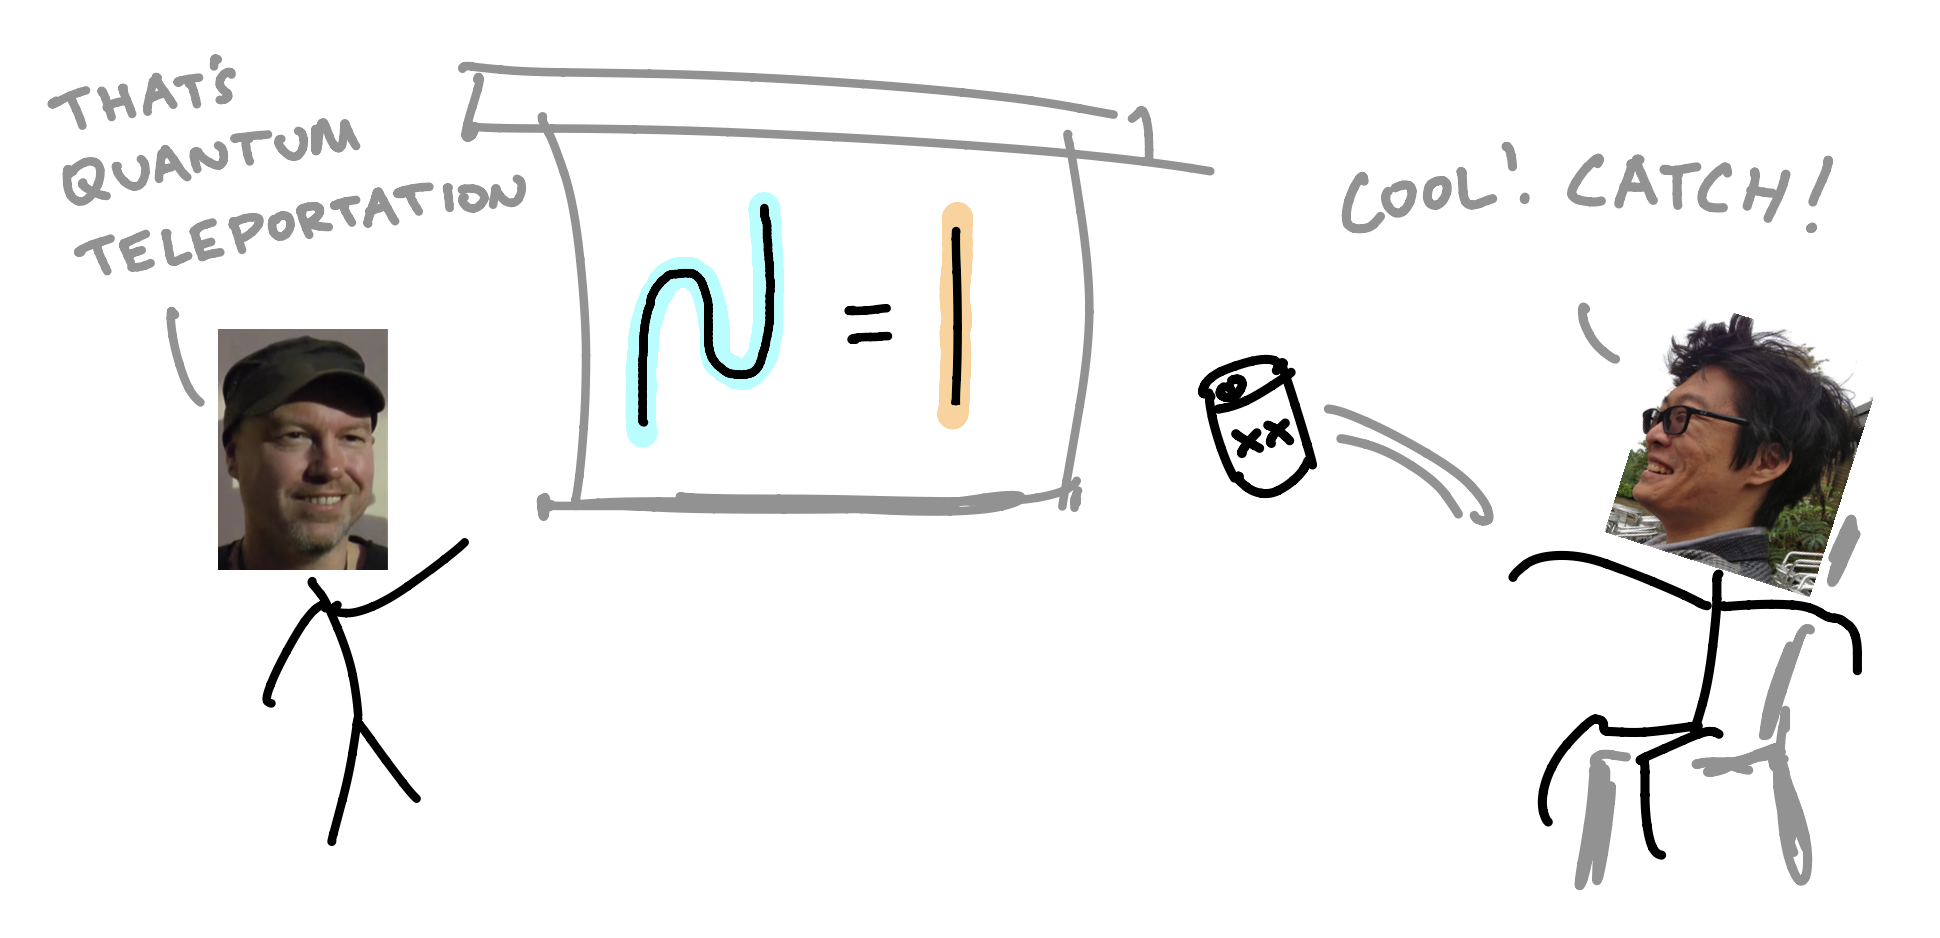
\includegraphics{figures/cartoons/v1}}
\caption{I met Bob in my master's in 2019, where he taught the picturing quantum processes course. When quantum teleportation was explained in half a minute by a diagram, I decided to pursue a DPhil in diagrammatic mathematics. In the last lecture, I threw Bob a cider, after which he seemed to like me. I did not know he was an alcoholic.}
\end{figure}
\clearpage

I was shanghaied into thinking about diagrams for language. I was deeply dissatisfied with the content from the standpoint my own intellectual integrity. Firstly, there seemed to me an unspoken claim that the presence of cups in pregroup diagrams (which implied a noncartesian and hence large tensor product) made it necessary to use quantum computers to effectively compute pregroup diagrams. I just could not believe that my brain required quantum computation to understand language. This implicit claim of kinship between quantum and linguistics was further entrenched by the analysis of the relative pronoun in terms of frobenius algebras, since spiders in $\mathbf{Vect}^\otimes$ were the \emph{sine qua non} of categorical quantum mechanics. The best steelman for spiders I have is that frobenius algebras (which are central to bicategories of relations \bR CITE \e) just happen to be a ubiquitous mathematical structure that are well-suited to express the mathematics of connections, both in language and in quantum.\\

Second, representing the content of a sentence as a vector in a sentence-vector-space did not sit well with me, since this move meant that the only meaningful thing one could do with two sentences was take their inner-product as a measure of similarity. Moreover, I had the theoretical concern that language is in principle indefinitely productive, so one could construct a sentence that marshalled indefinitely many nouns, and at some point for any finite vector space $s$ one would run out of room to encode relationships, or else they would be cramped together in a way that did not suit intuitions about the freedom of constructing meanings using language. I always believed in the existence of a simple, practical, and intuitive categorical, compositional, and distributional semantics; I just didn't believe that the role of quantum -- however helpful or interesting -- was \emph{necessary}.

My first unsatisfactory attempt was in my Master's thesis \bR CITE \e. It had been known for a while that a free autonomous category construction by Delpeuch \bR CITE \e could potentially eliminate some of the cups in pregroup diagrams, yielding what amounted to a method to transform a pregroup diagram into a monoidal string diagram in the shape of a context-free grammar tree. This trick had the limitation that freely adding directed cups and caps to a string diagrammatic signature did not turn a symmetric monoidal category into a (weakly) compact closed one, rather just into a monoidal category where the original wires had braidings, but all the new left and right dual wires did not; this presented difficulties in accounting for iterated duals for higher-order modifiers such as adverbs in grammatical types, and had nothing to say about spiders. I tried to generalise this trick to `freely' adding arbitrary diagrammatic gadgets to string diagrams, but my assessor Samson pointed out that it was nontrivial to determine whether such constructions were faithful. In retrospect the free autonomous completion of a parameterised \bR CITE \e markov category \bR CITE \e is in the ballpark of dequantumfying pregroup diagrams, but I didn't learn about them until later, and that still wouldn't have addressed the issues that come with only having a sentence-wire.

\begin{figure}[h!]
\centering
\scalebox{1}{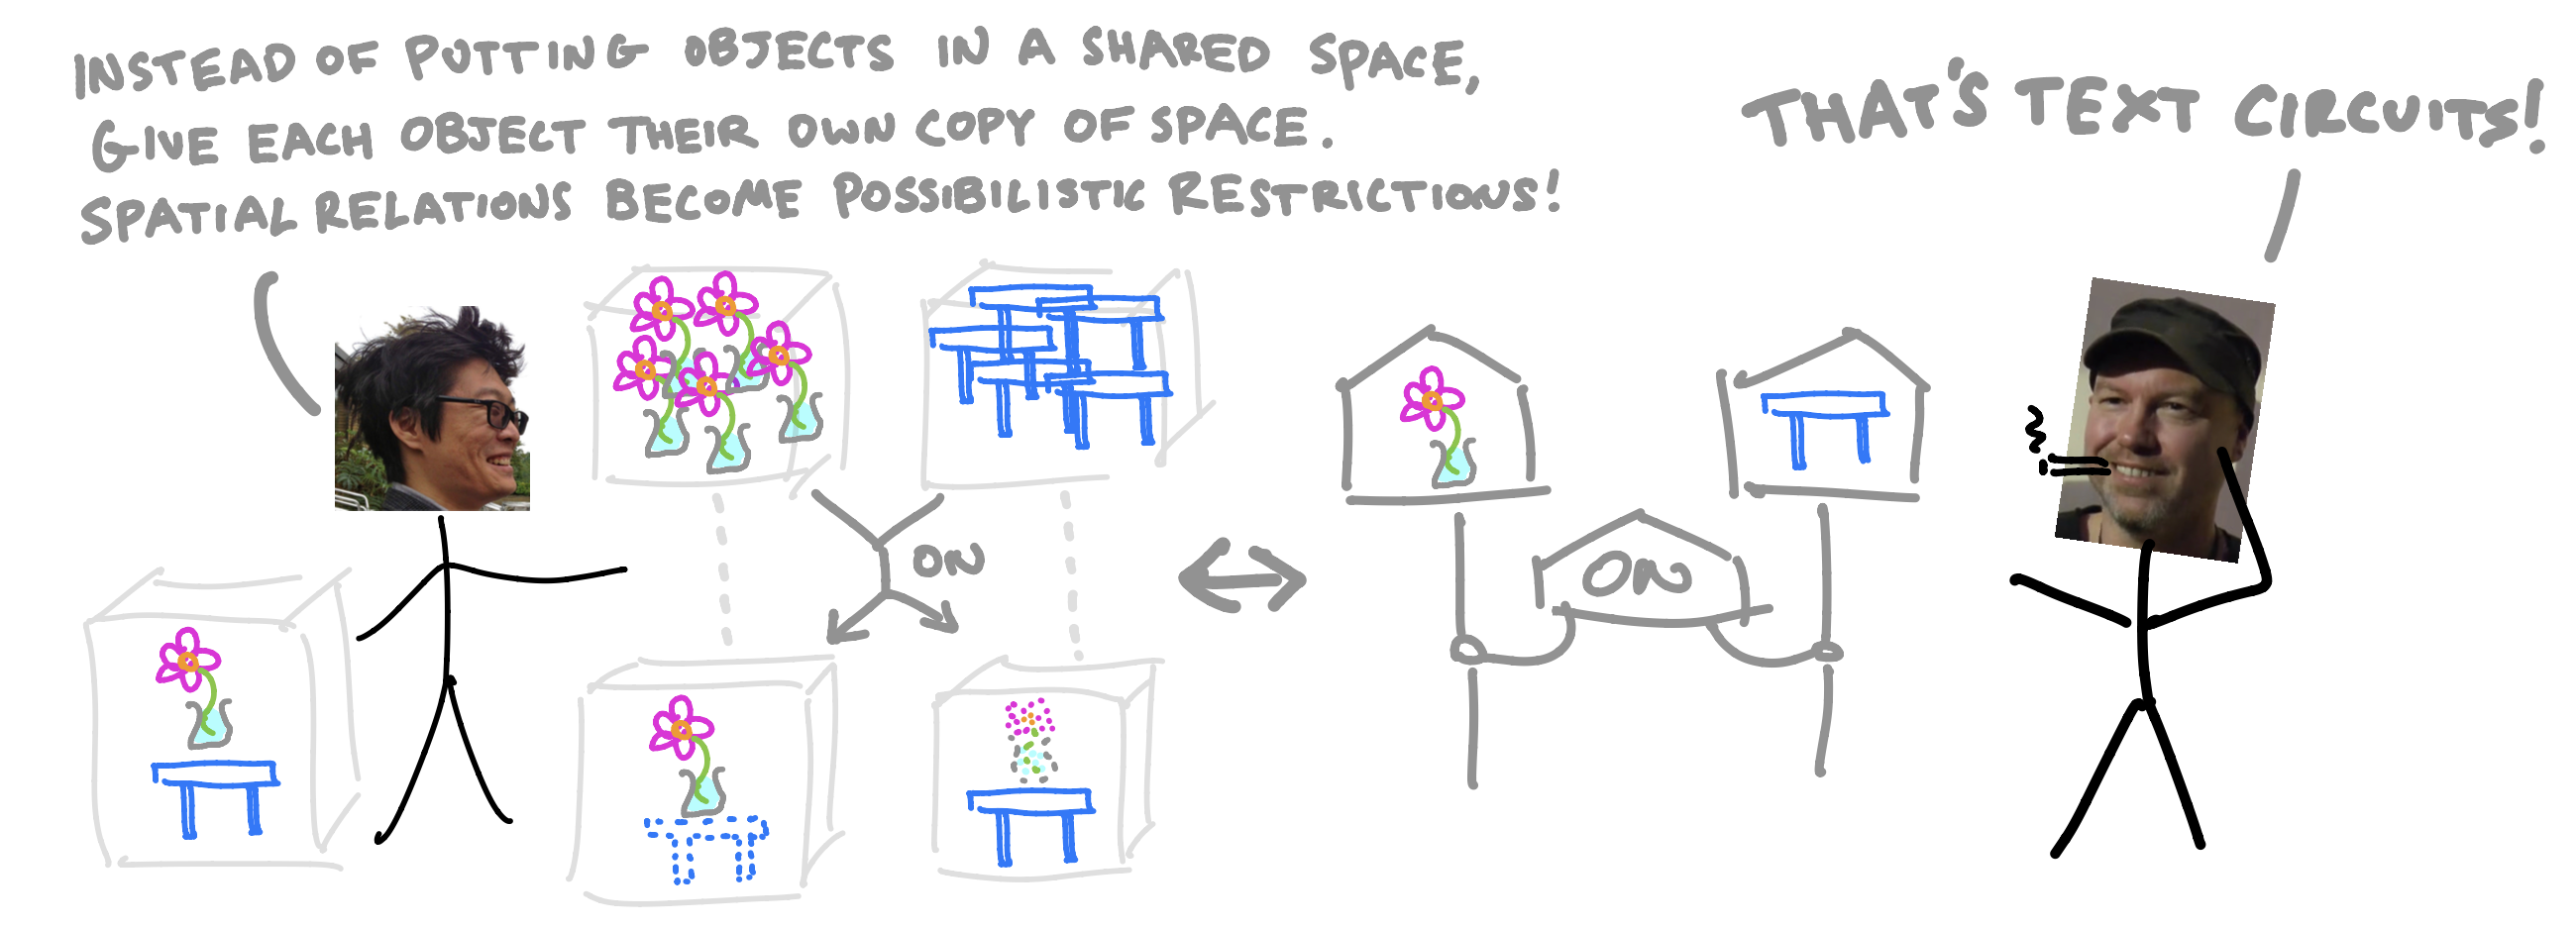
\includegraphics{figures/cartoons/circify1}}
\caption{Then COVID happened. During the first lockdown, I visited Bob's garden under technically legal circumstances, and I suggested a solution to the longstanding problem of representing linguistic spatial relationships. My theoretical concern was the culprit: the initial attempts at the problem failed because the approach was to find a single sentence object $s$ in which one could paste the data of arbitrarily many distinct spatial entities. The simple solution was a change in perspective.}
\end{figure}

\begin{figure}[h!]
\centering
\scalebox{1}{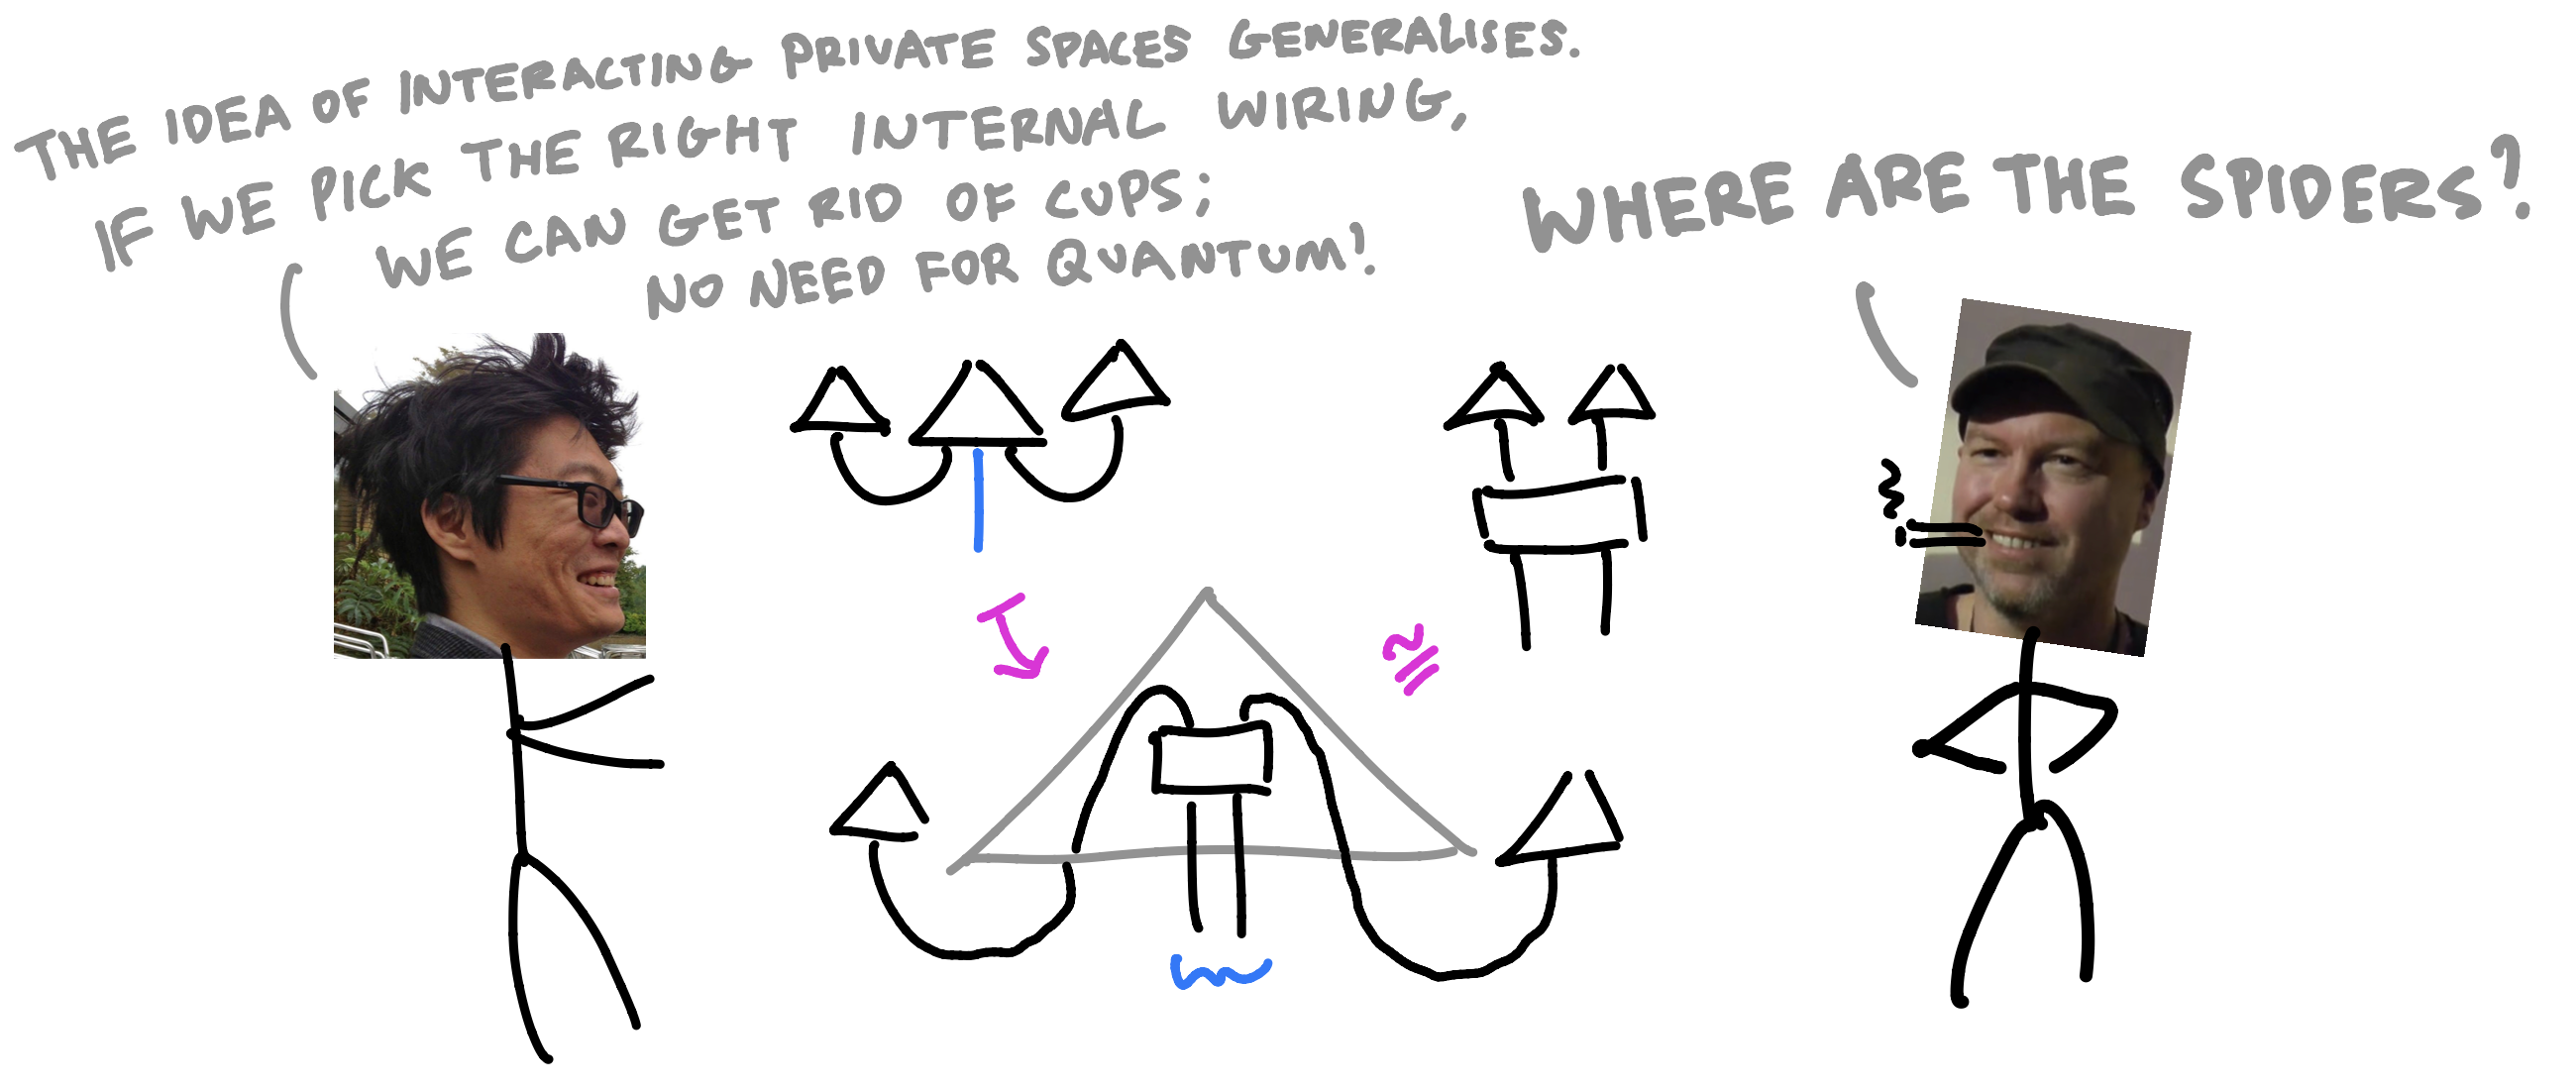
\includegraphics{figures/cartoons/circify2}}
\caption{That this move of splitting up the sentence-wire into a sentence-dependent collection of wires was sufficient to solve what had appeared to be a difficult problem prompted some re-examination of foundations. The free autonomisation trick in conjunction with sentence-wire-as-tensored-nouns seemed promising, but it became clear that right way to drown a DisCoCat thoroughly was to explain and eliminate the spiders.}
\end{figure}

\begin{figure}[h!]
\centering
\scalebox{1}{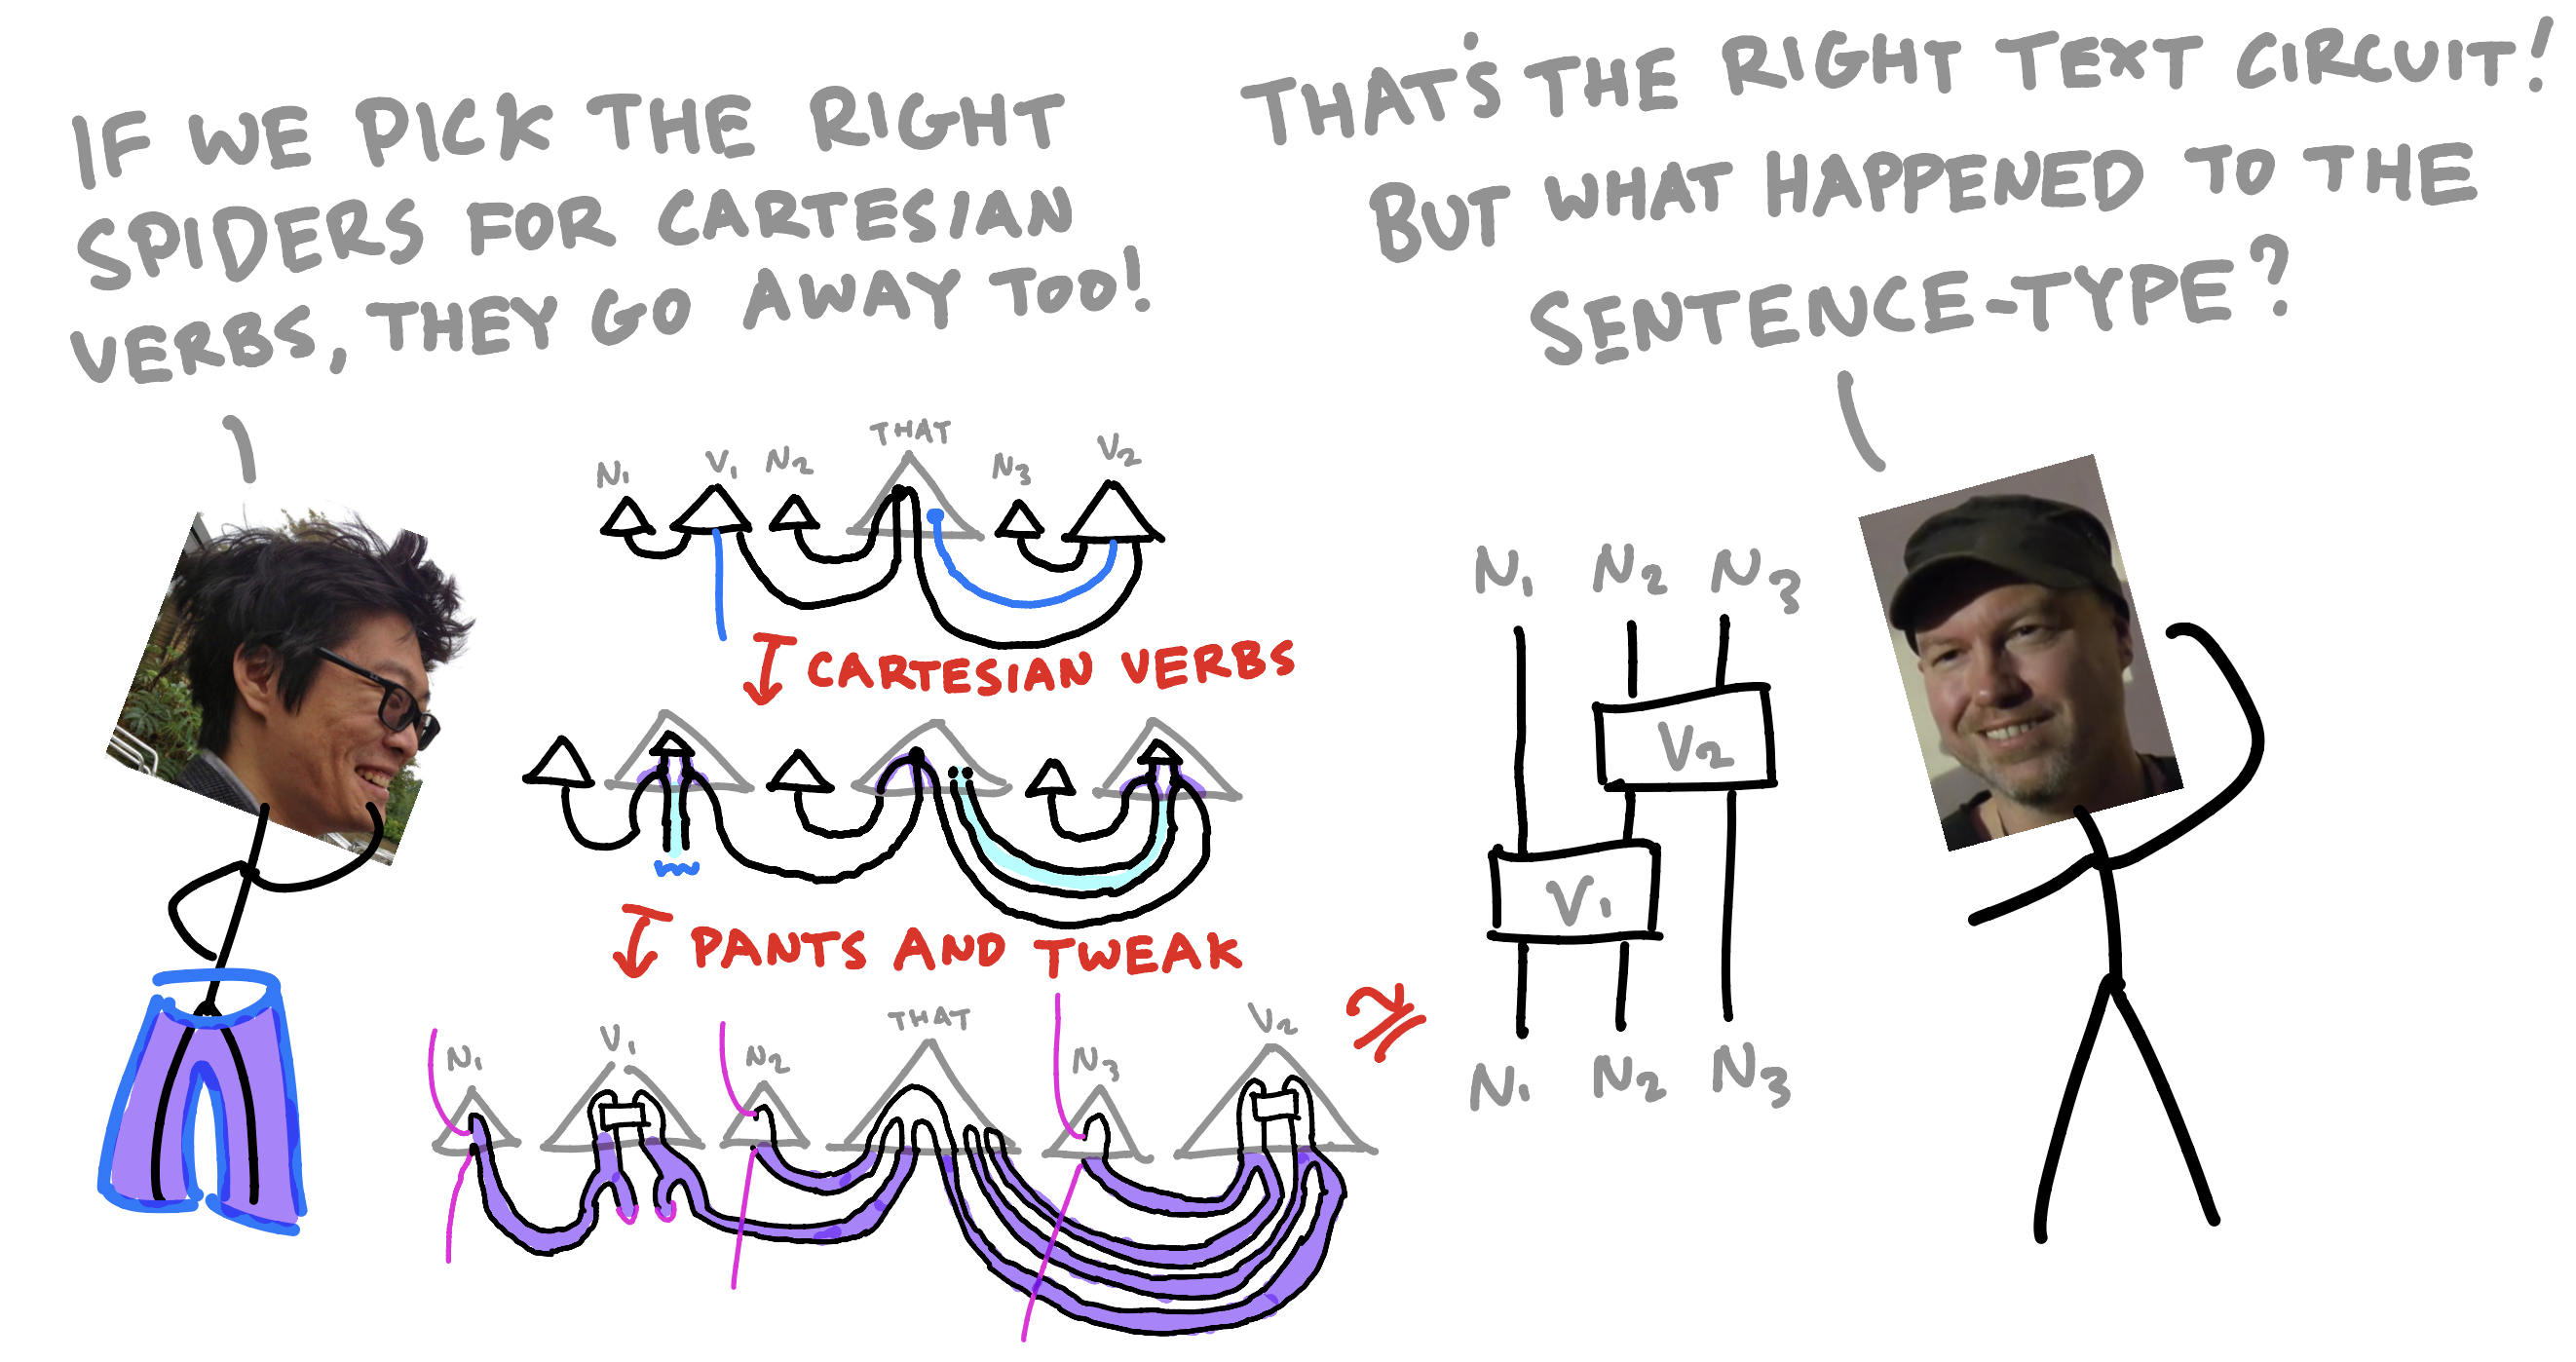
\includegraphics{figures/cartoons/circify3}}
\caption{I then discovered that by interpreting spiders as the well-known "pair of pants" algebra in a compact closed monoidal setting allowed for a procedure in which the final form was purely symmetric monoidal -- the absence of cups and caps meant that there was no practical necessity to interpret diagrams on quantum computers: any computer would suffice. The role of spiders for relative pronouns was illuminated in the presence of splitting the sentence wire: the pair-of-pants are the algebra of morphism composition, and splitting the sentence wire into a collection of nouns allowed relative-pronoun-spiders to pick out the participating nouns to compose relationships onto.}
\end{figure}

\begin{figure}[h!]
\centering
\scalebox{1}{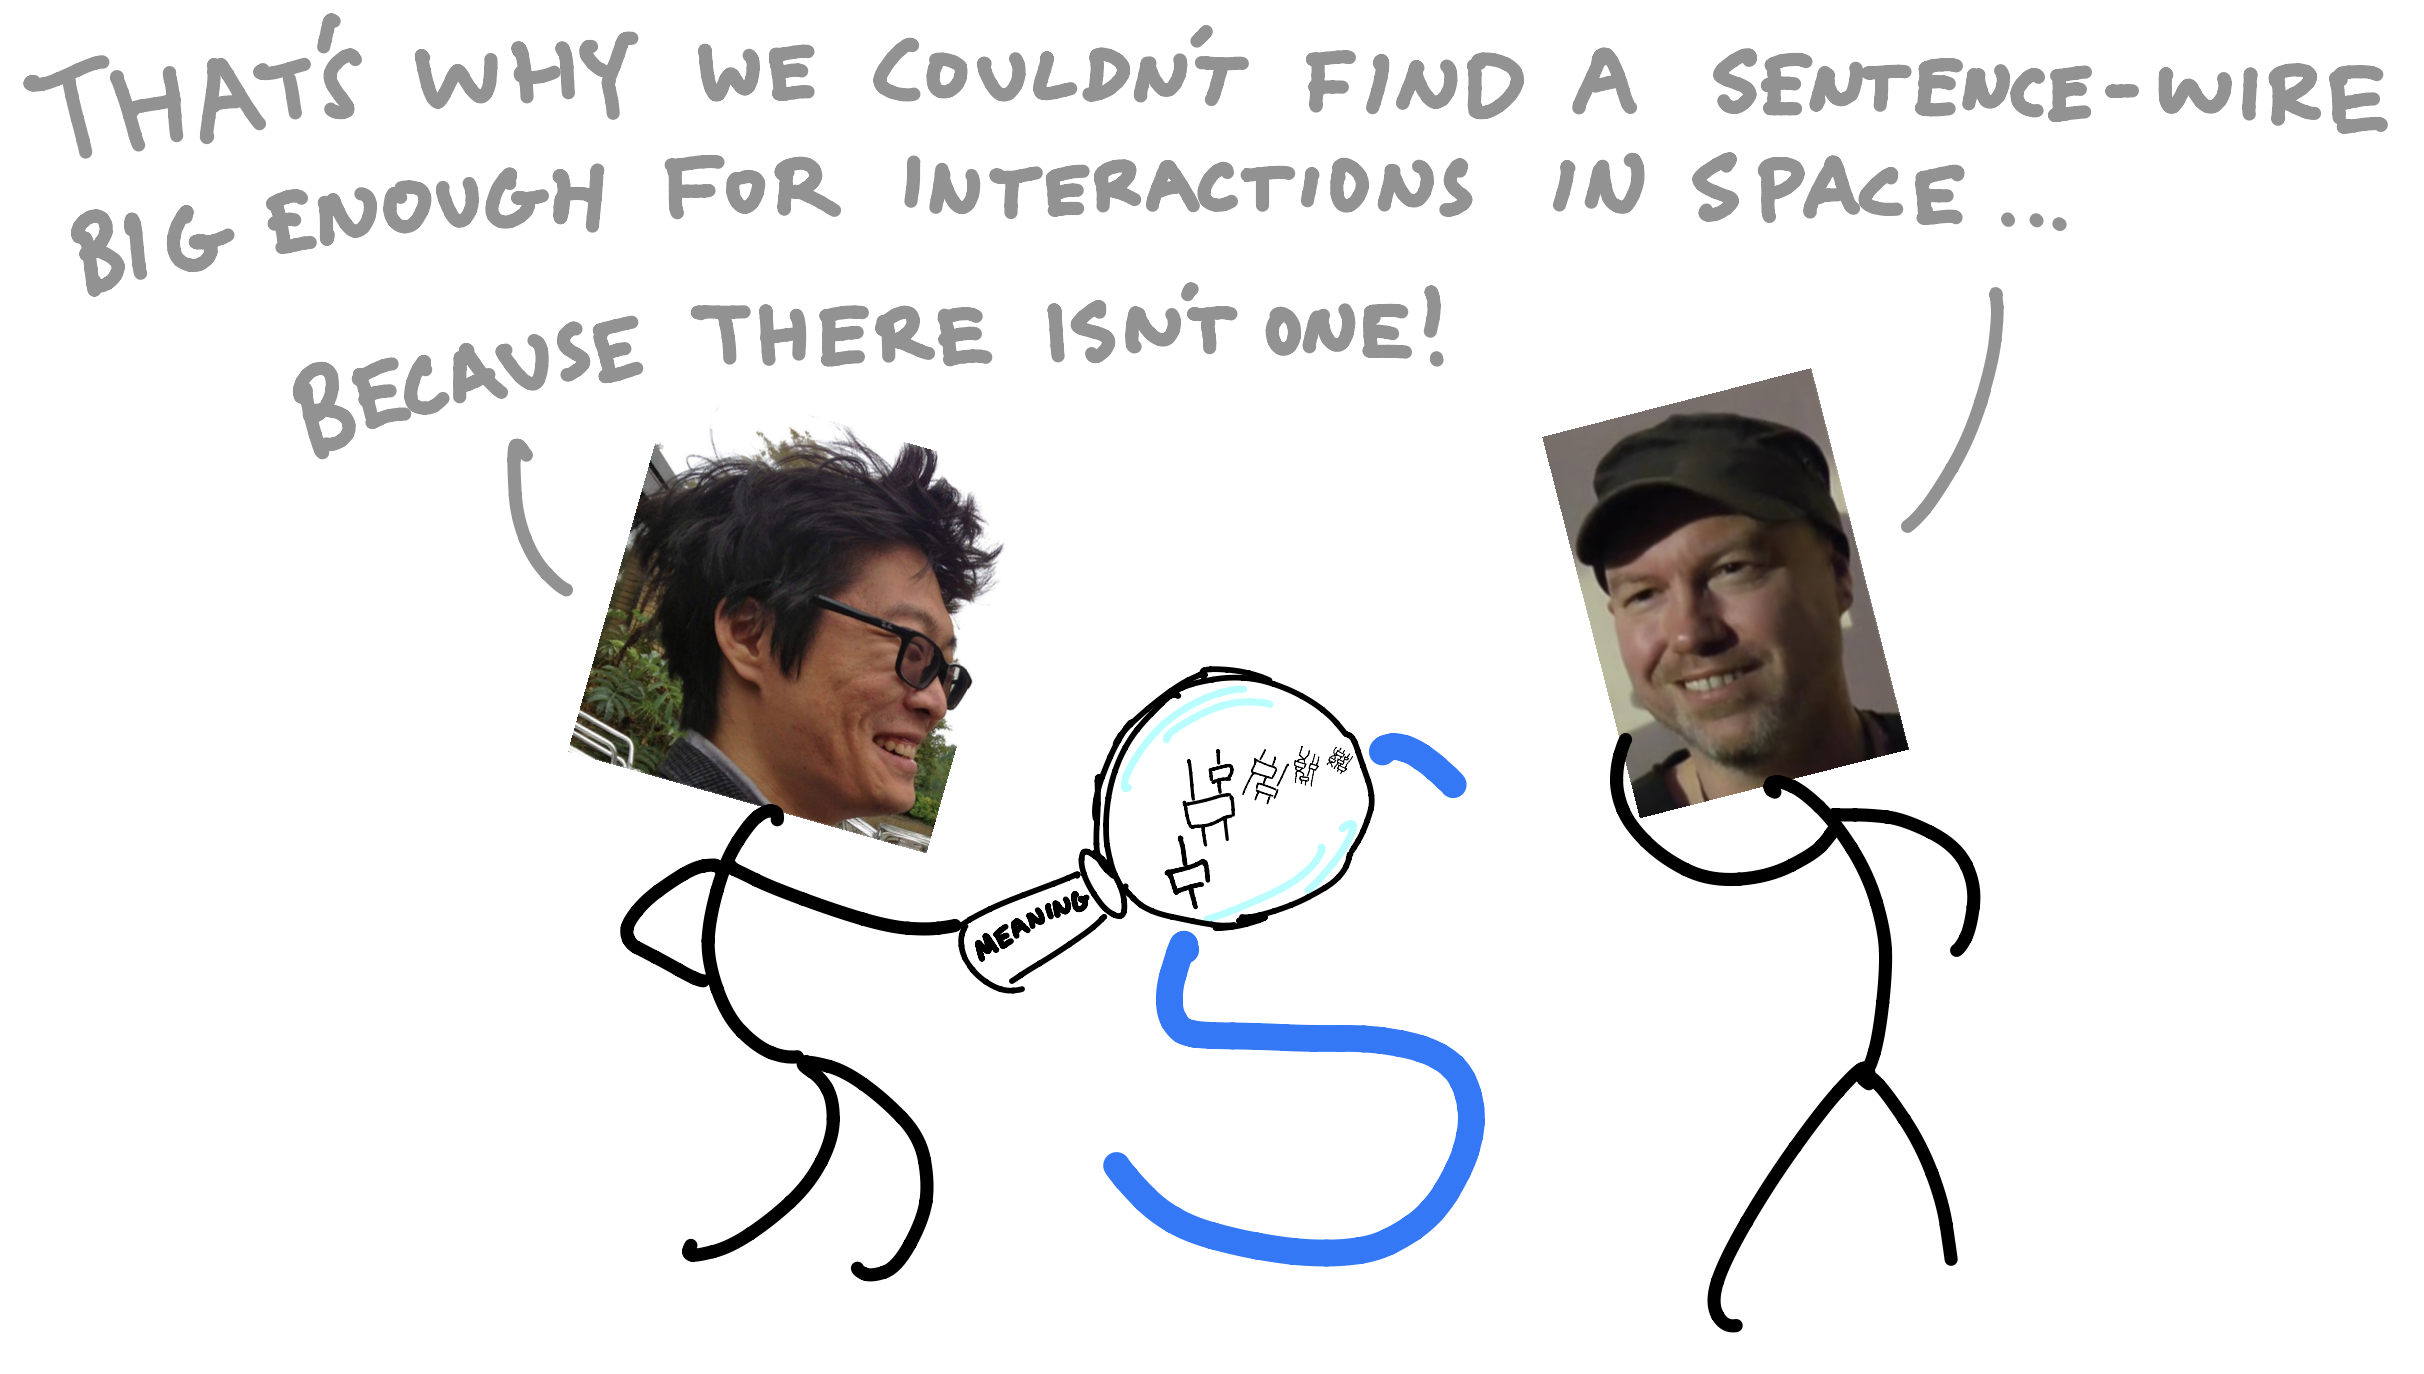
\includegraphics{figures/cartoons/nosent}}
\caption{A coherent conservative generalisation of DisCoCat with less baggage had emerged, or rather, DisCoCirc was placed to formally subsume DisCoCat. It was now understood that the sentence type was a formal syntactic ansatz for the sake of grammar, which was to be interpreted in the semantic domain not as a single wire, but as a sentence-dependent collection of wires. It was further realised that the complexity of pregroup diagrams was due to grammar -- the topological deformation of semantic connections to fit the one-dimensional line of language -- whereas the essential connective content of language could be expressed in a simple form that distilled away the bureaucracy of syntax.}
\end{figure}

\begin{figure}[h!]
\centering
\scalebox{1}{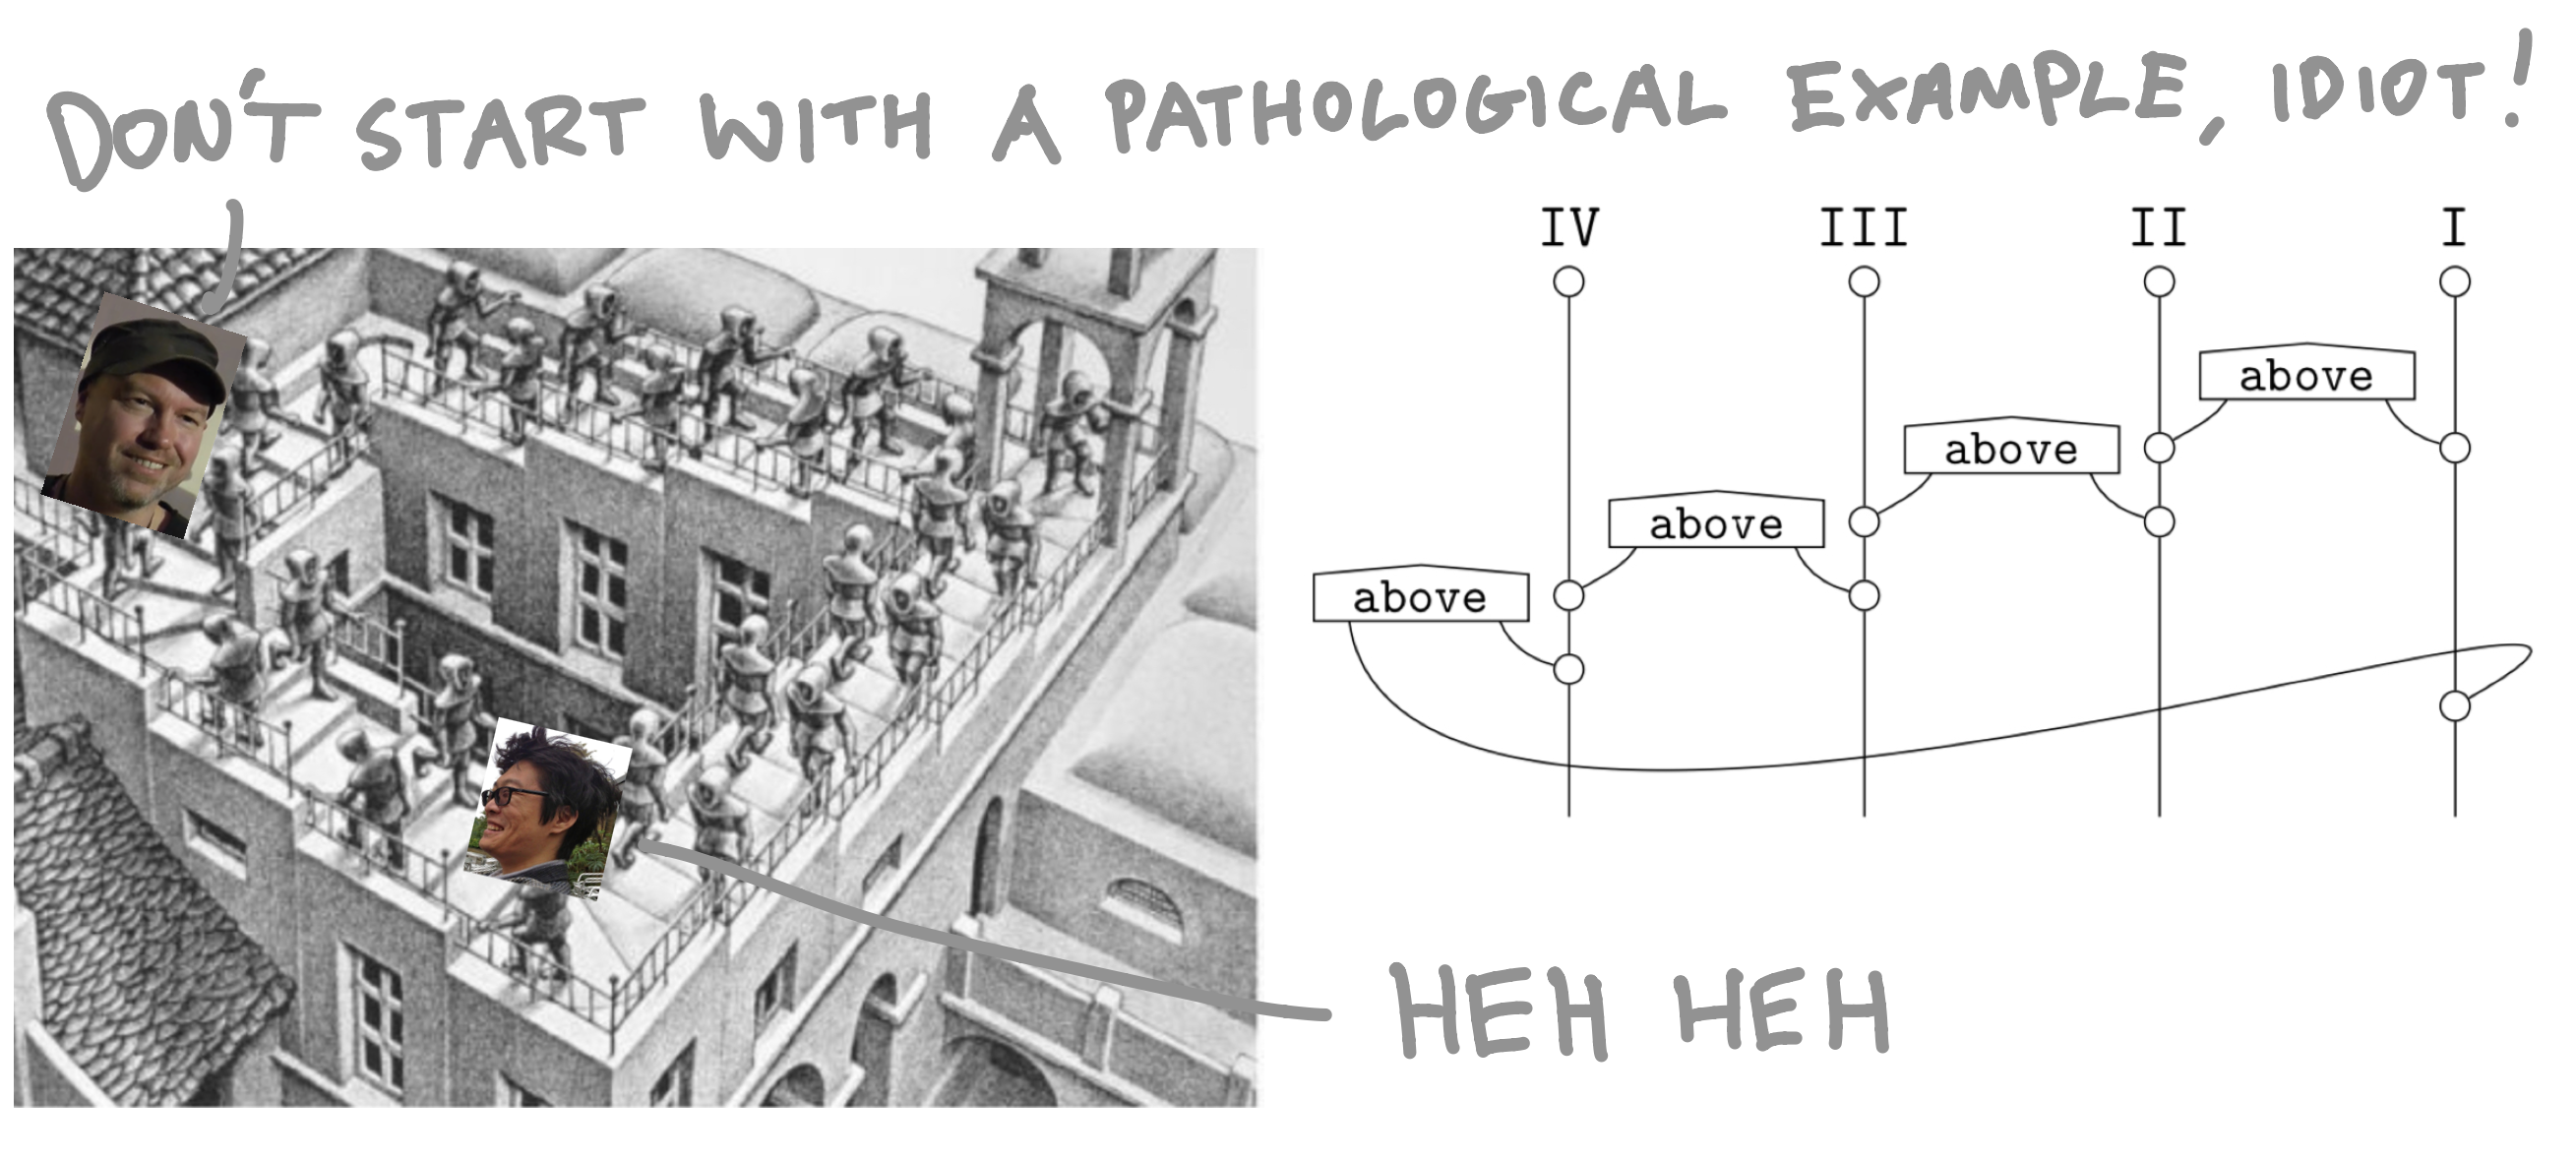
\includegraphics{figures/cartoons/space1}}
\caption{We wrote up the story about spaces in \bR CITE \e, the spiritual successor to \emph{interacting conceptual spaces I}. We could formally calculate the meanings of sentences that used linguistic spatial relations, all using a simple and tactile diagrammatic calculus.}
\end{figure}

\begin{figure}[h!]
\centering
\scalebox{1}{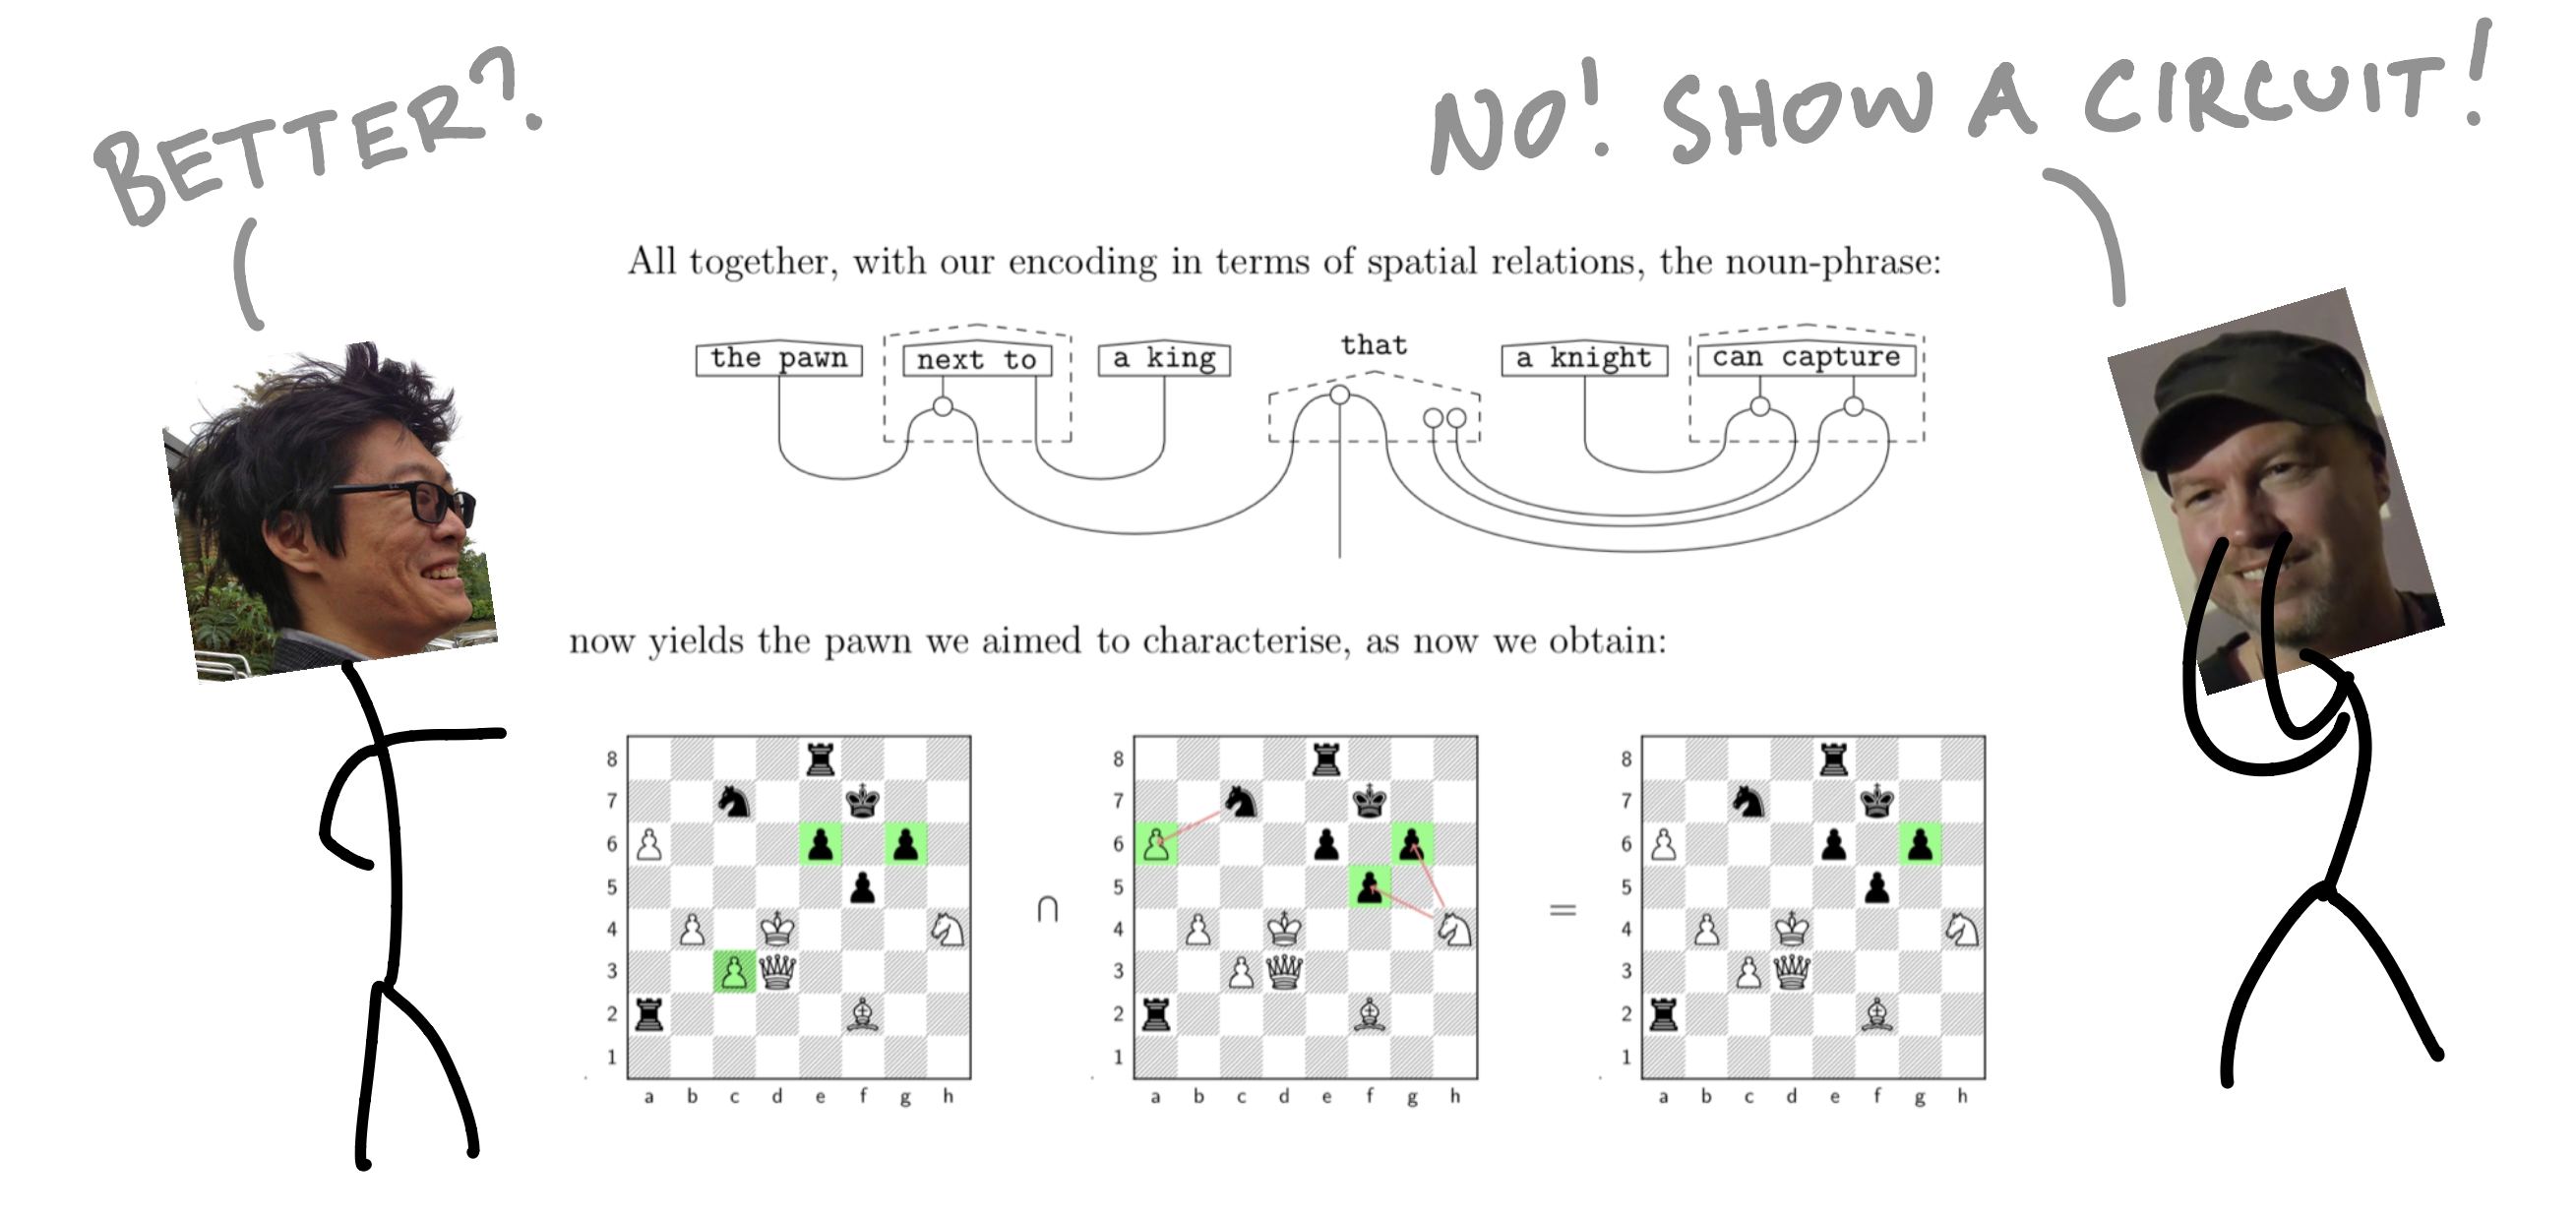
\includegraphics{figures/cartoons/space2}}
\end{figure}

\begin{figure}[h!]
\centering
\scalebox{1}{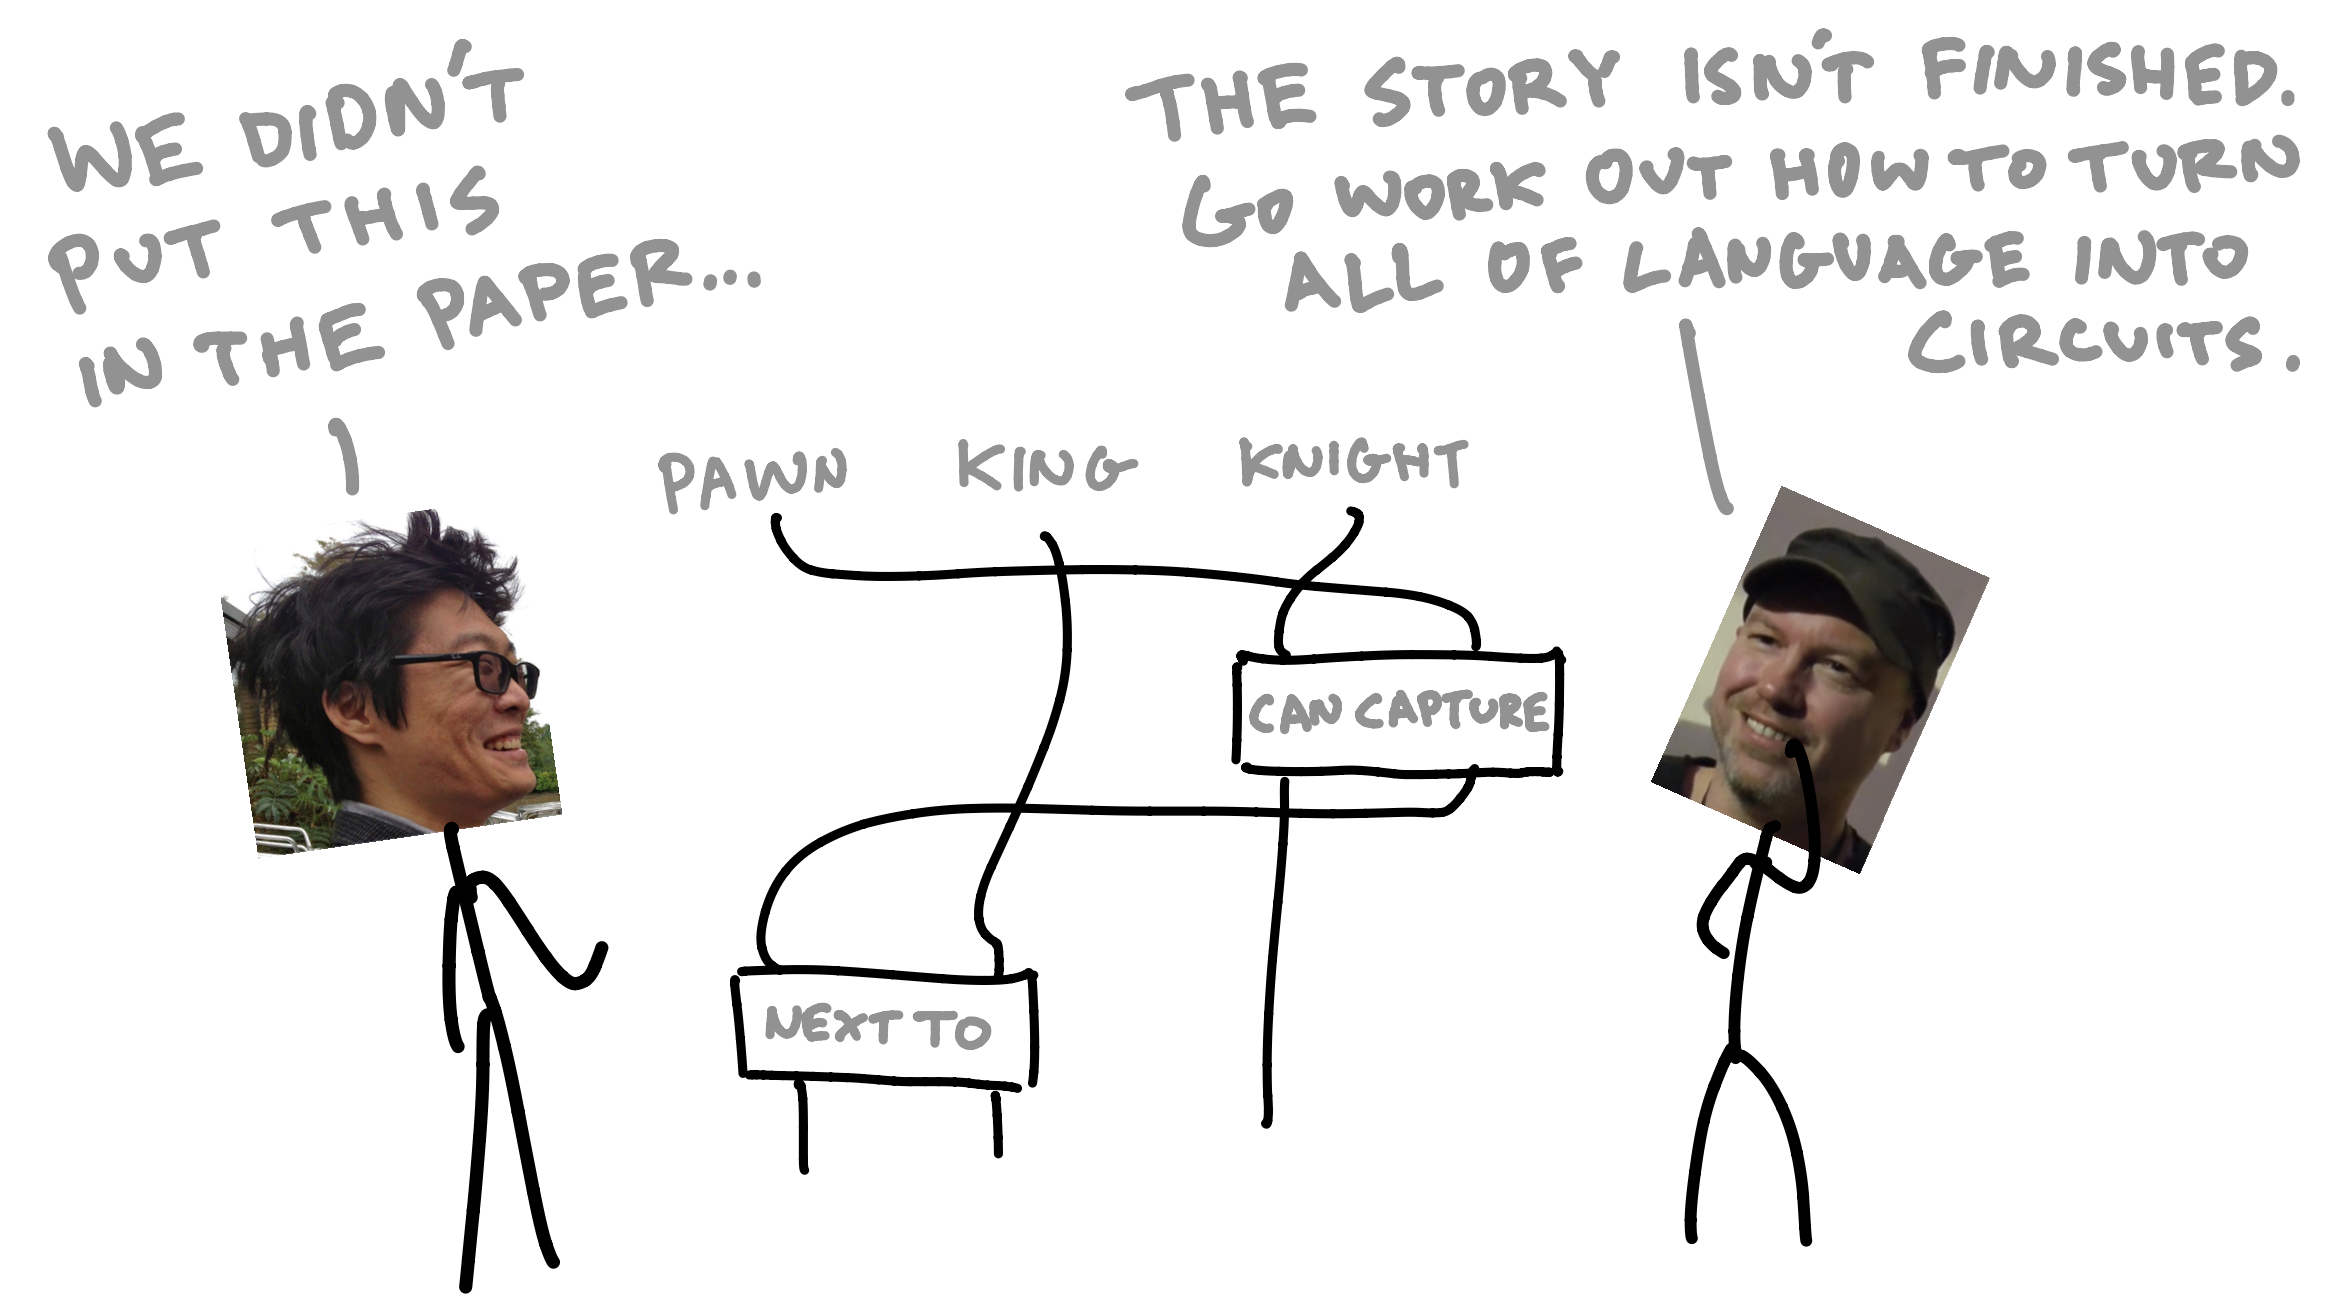
\includegraphics{figures/cartoons/space3}}
\caption{The paper on spatial relations actually came very late, because I was busy with Bob's ludicrous request to go turn "all of language" into circuits. I bitched and moaned about how I wasn't a linguist and how it was an impossible task, but I was in too deep to back out.}
\end{figure}

\begin{figure}[h!]
\centering
\scalebox{1}{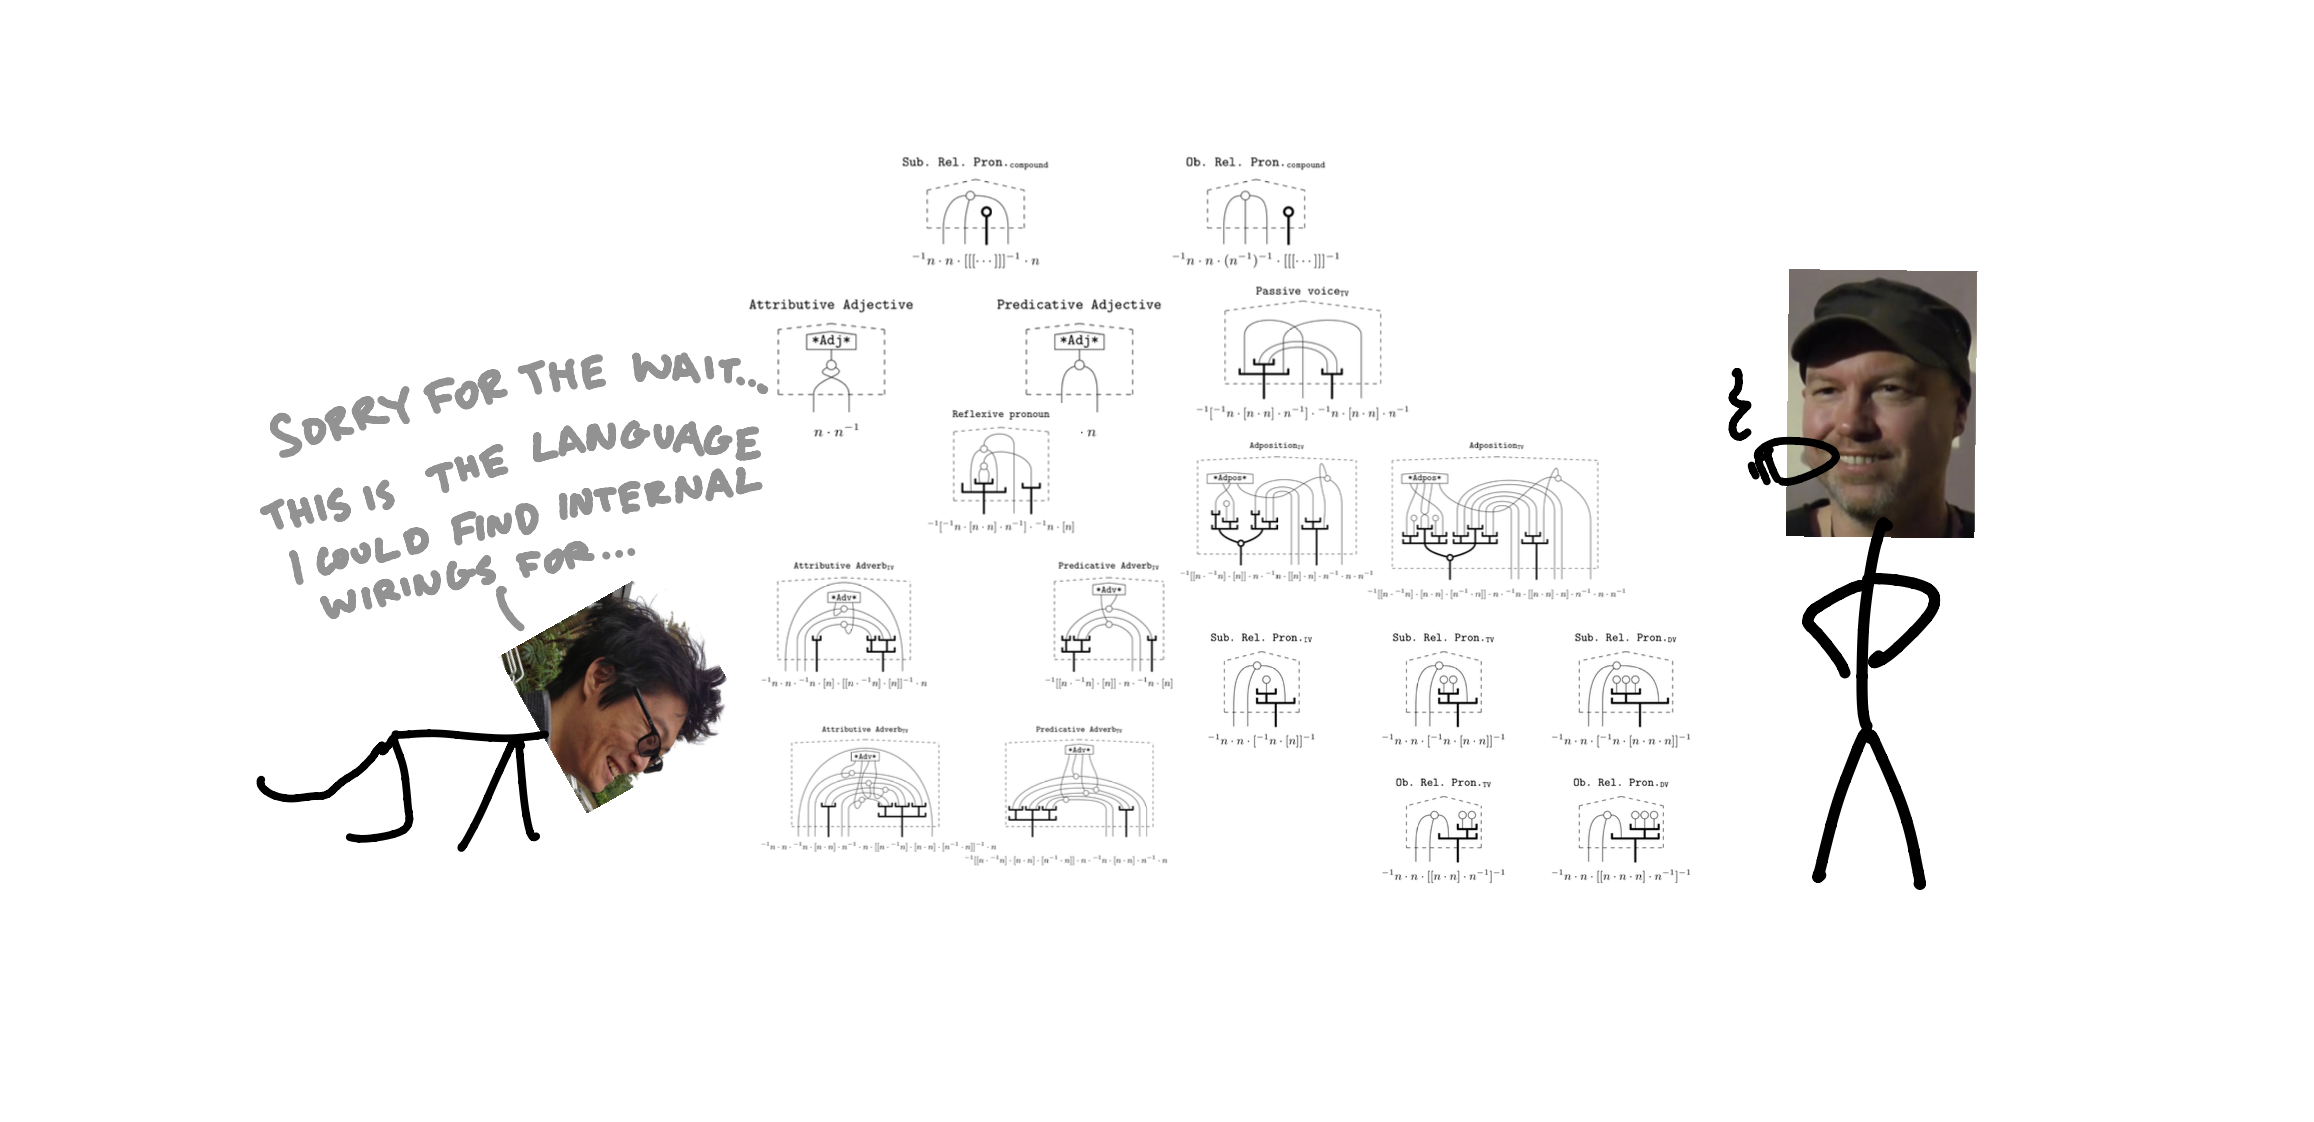
\includegraphics{figures/cartoons/pregroup1}}
\caption{I suppose the nice thing about aiming for the moon is that even failure might mean you leave orbit. So I settled for what I thought was a sensible fragment of English, for which I devised internal wirings and an algorithm that transformed pregroup diagrams with the internal wirings into circuit form. Many tiring diagrams later, I presented my results in the first draft of "distilling text into circuits".}
\end{figure}

\begin{figure}[h!]
\centering
\scalebox{1}{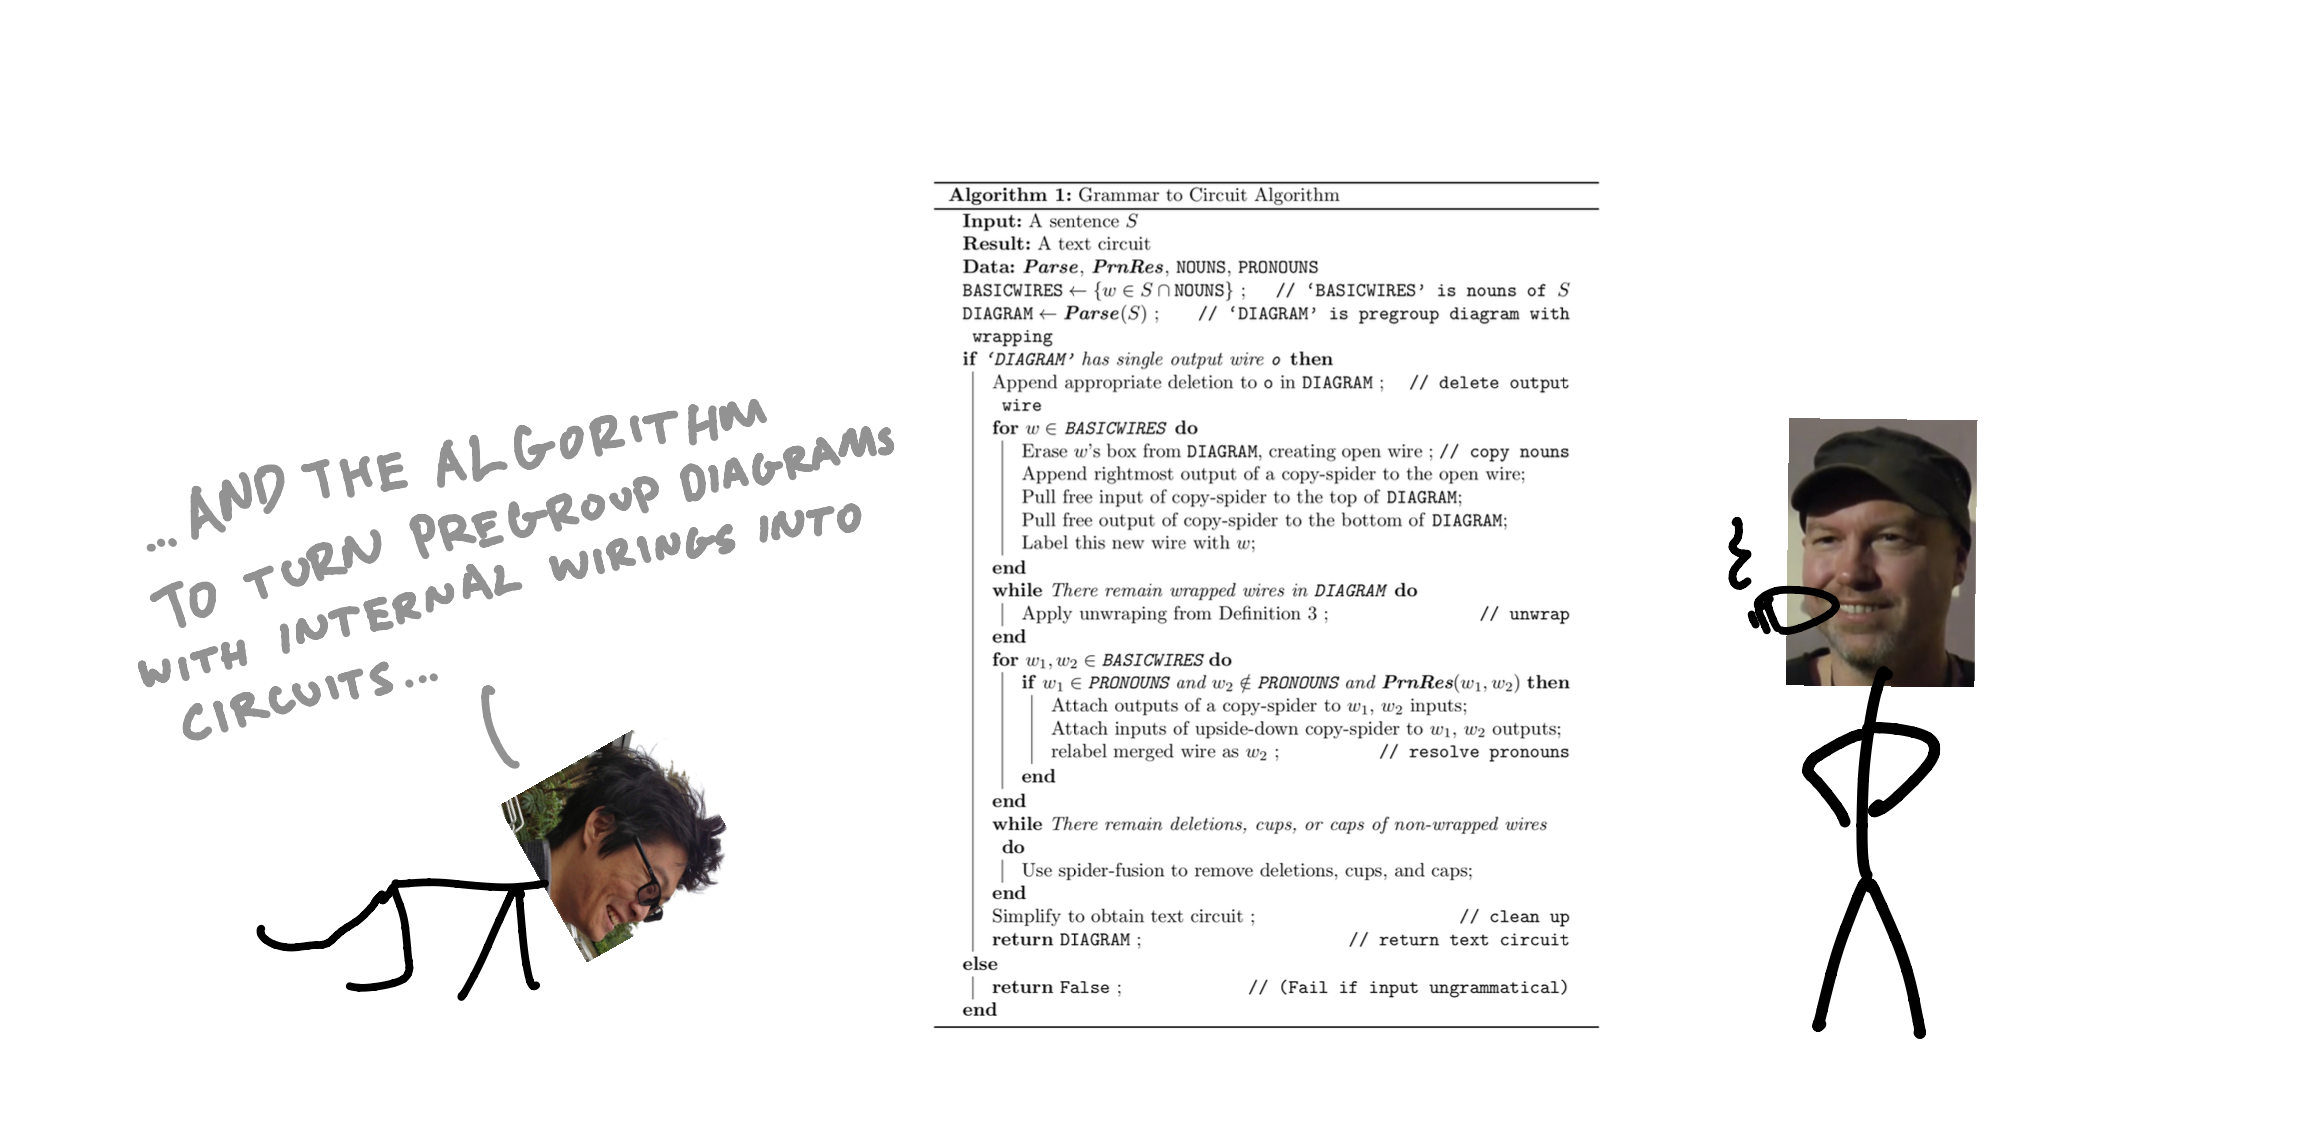
\includegraphics{figures/cartoons/pregroup2}}
\end{figure}

\begin{figure}[h!]
\centering
\scalebox{1}{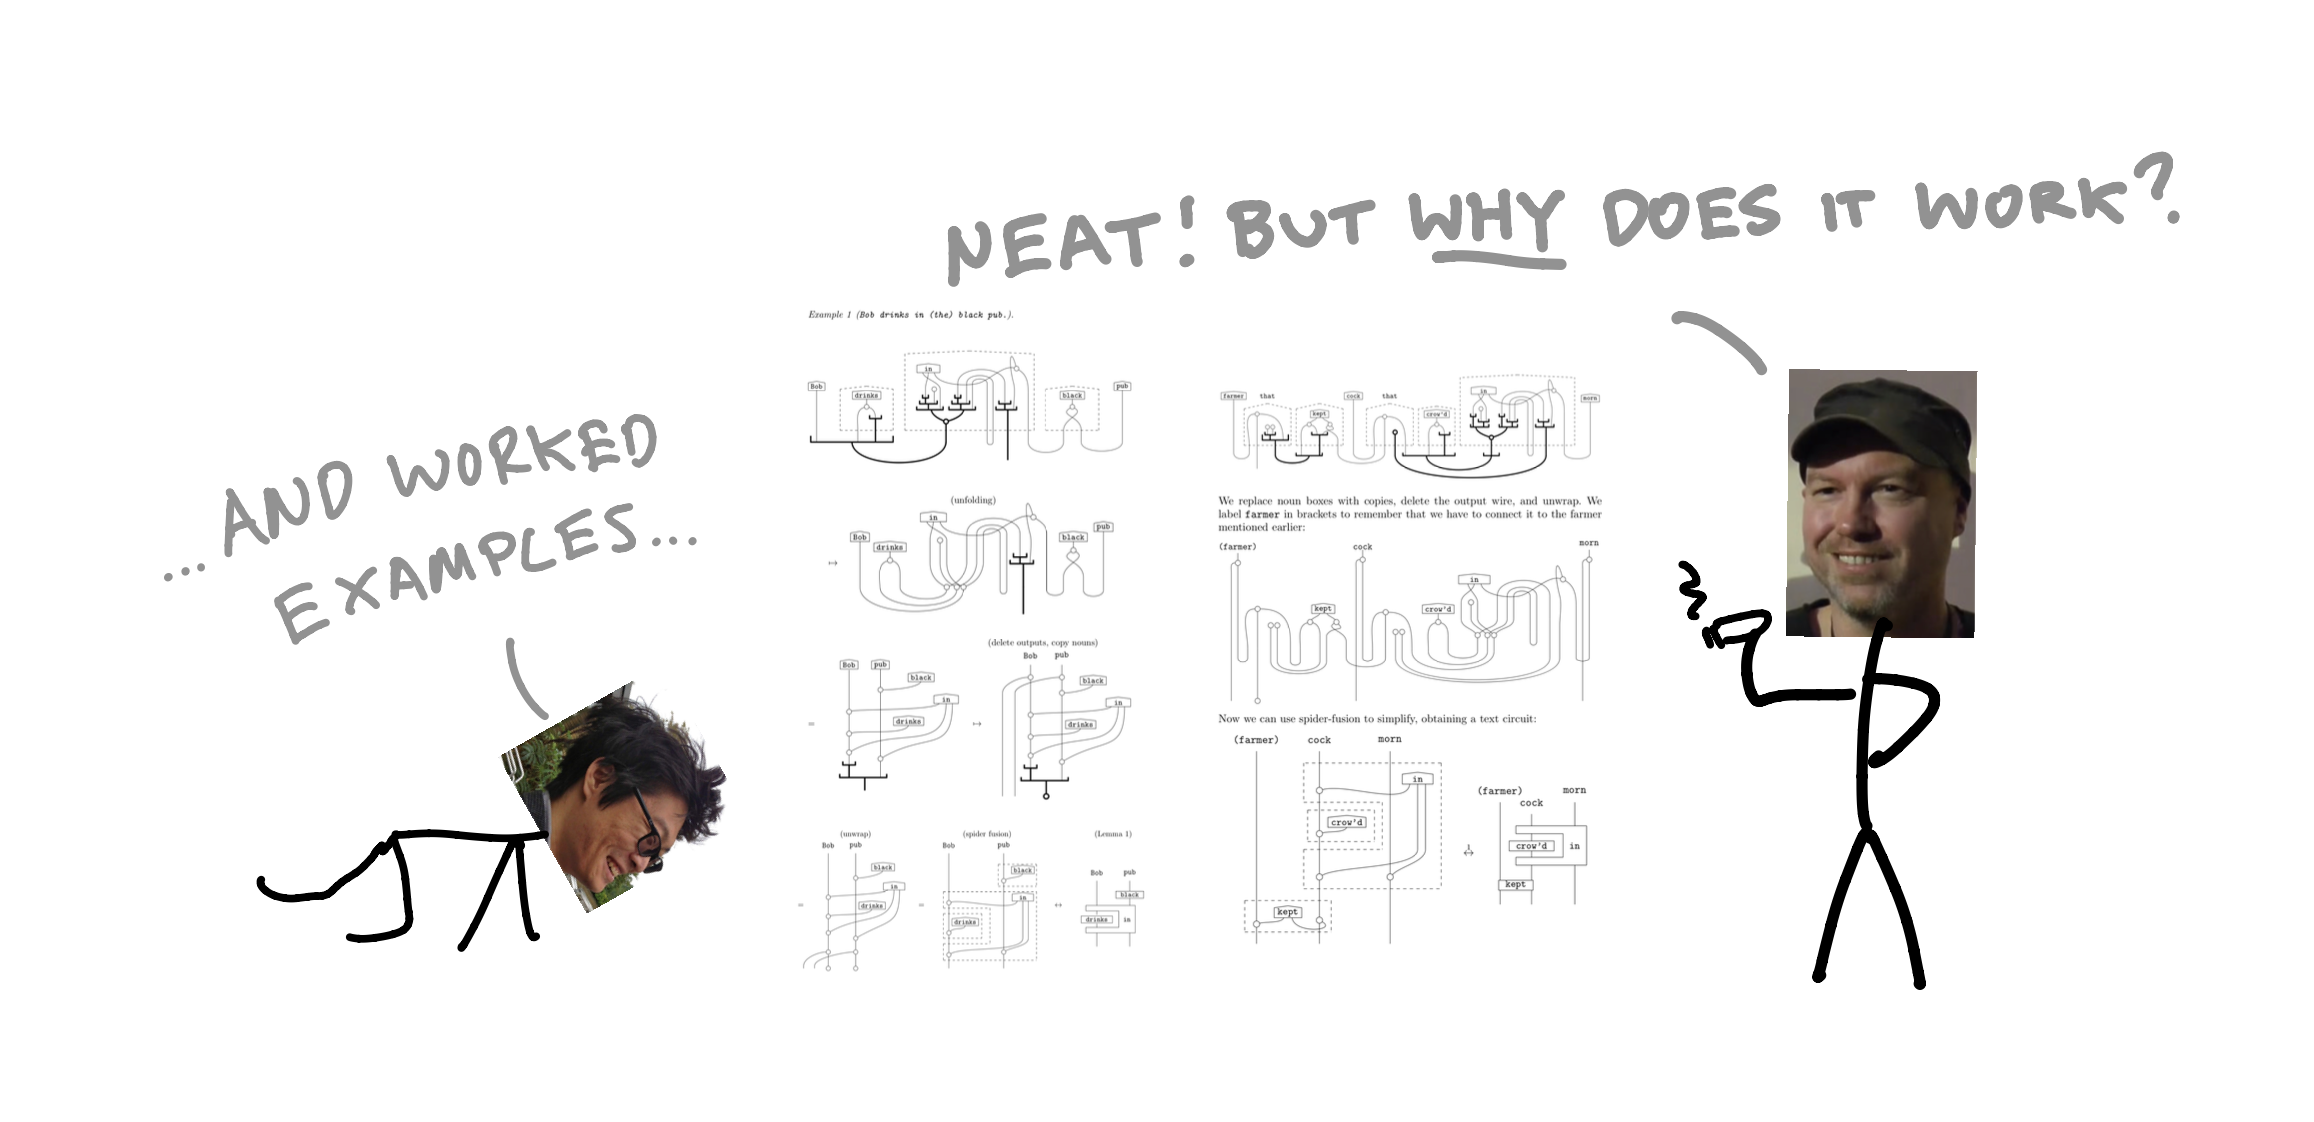
\includegraphics{figures/cartoons/pregroup3}}
\end{figure}

\begin{figure}[h!]
\centering
\scalebox{1}{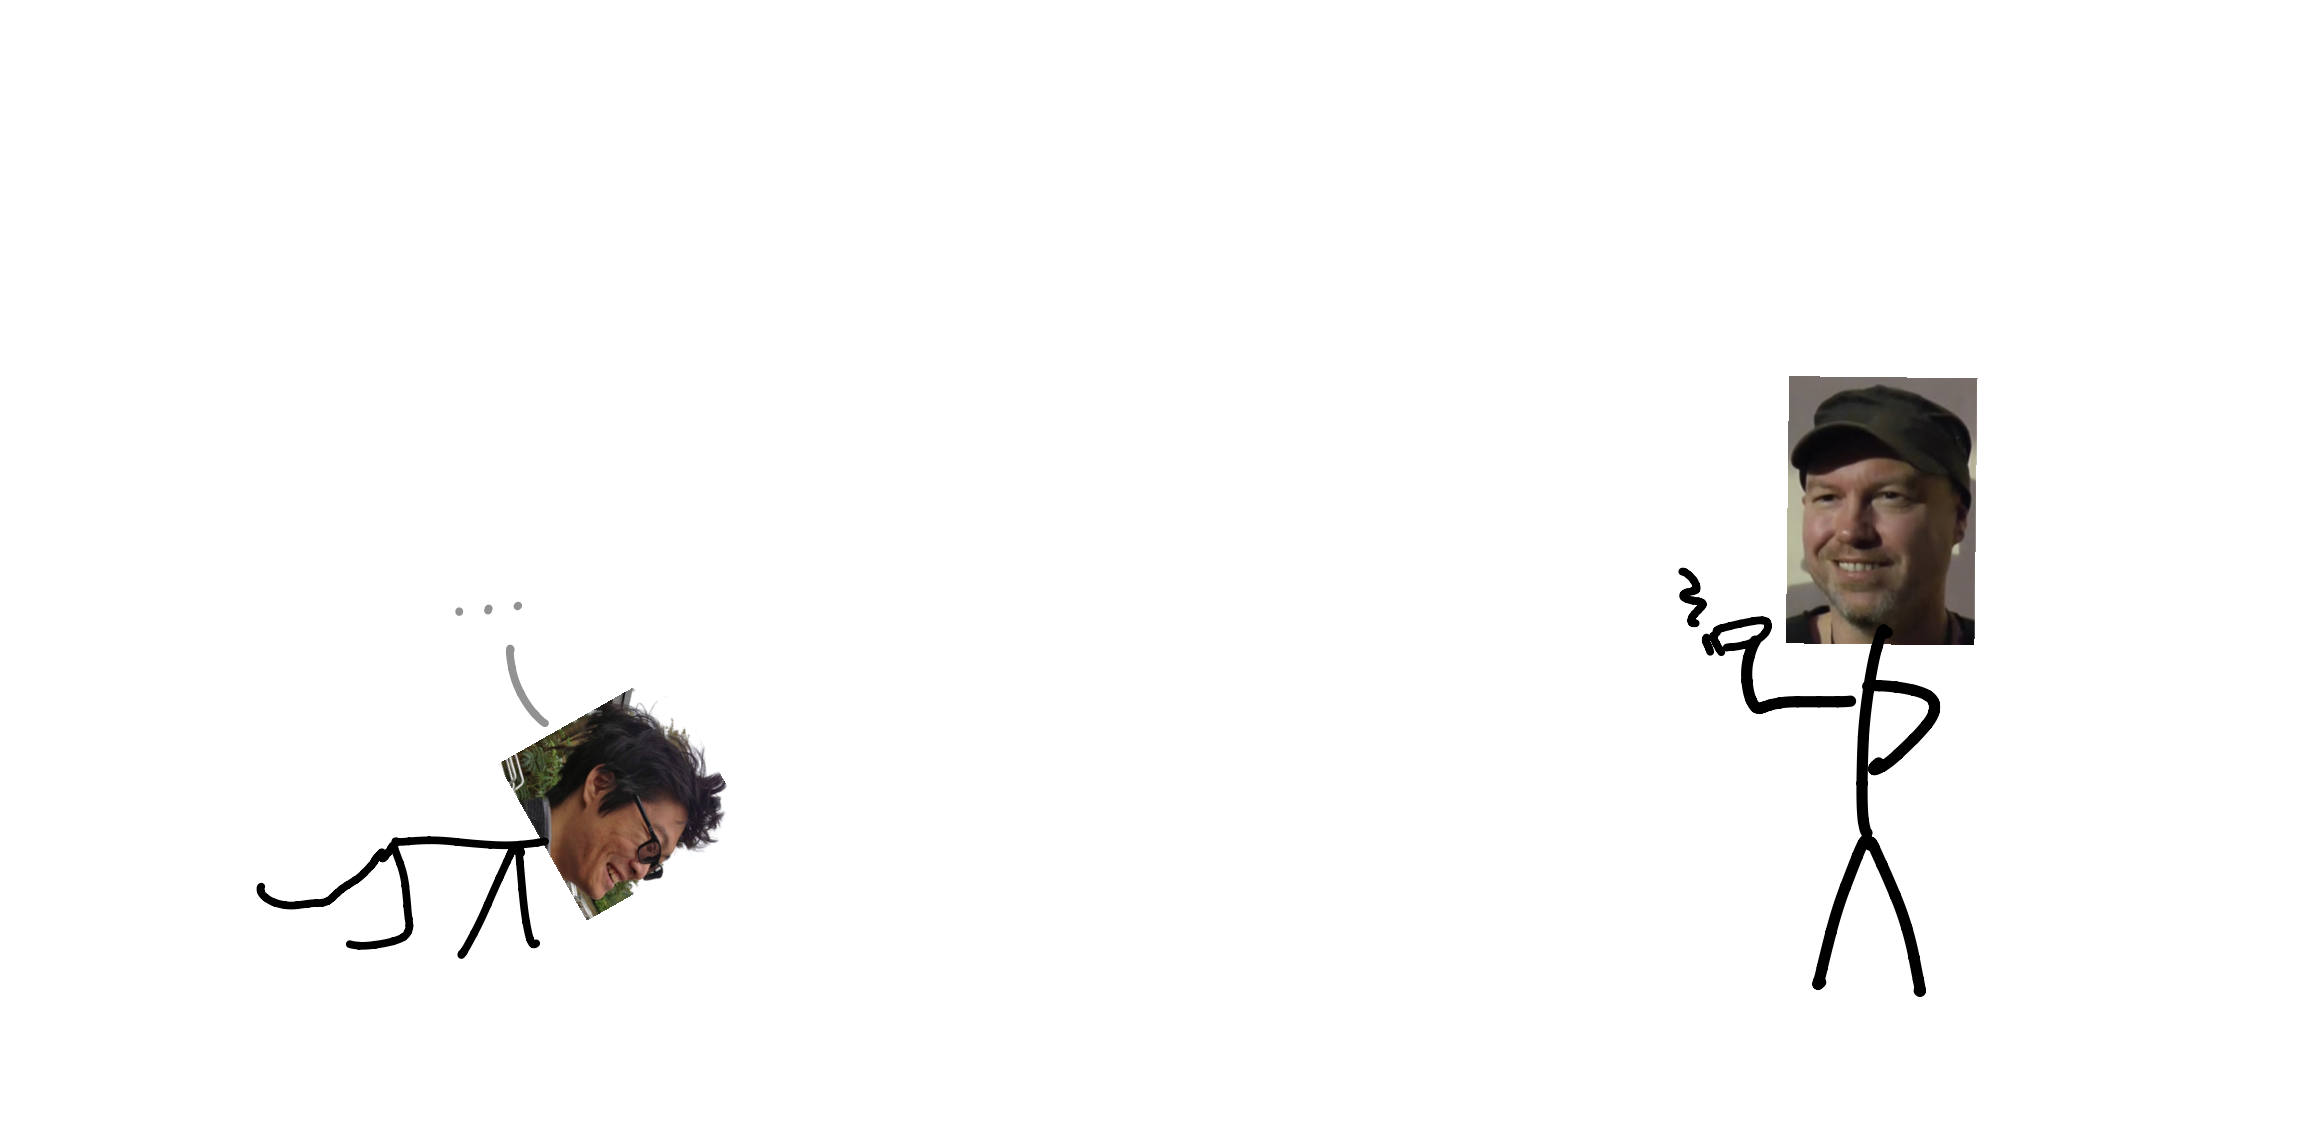
\includegraphics{figures/cartoons/pregroup4}}
\caption{Bob had a good point. Everything worked, but we had no understanding as to why, and accordingly, whether or not it would all break. At this point in time, Jonathon Liu, who was a masters' student I taught during COVID, had committed the error of thinking diagrams were cool, and was now hanging out with me and Bob. After understanding the procedure, Jono independently devised the same arcane internal wirings as I had, but neither of us could explain how we did it. So we had evidence of an underlying governing structure that was coherent but inarticulable.}
\end{figure}

\begin{figure}[h!]
\centering
\scalebox{1}{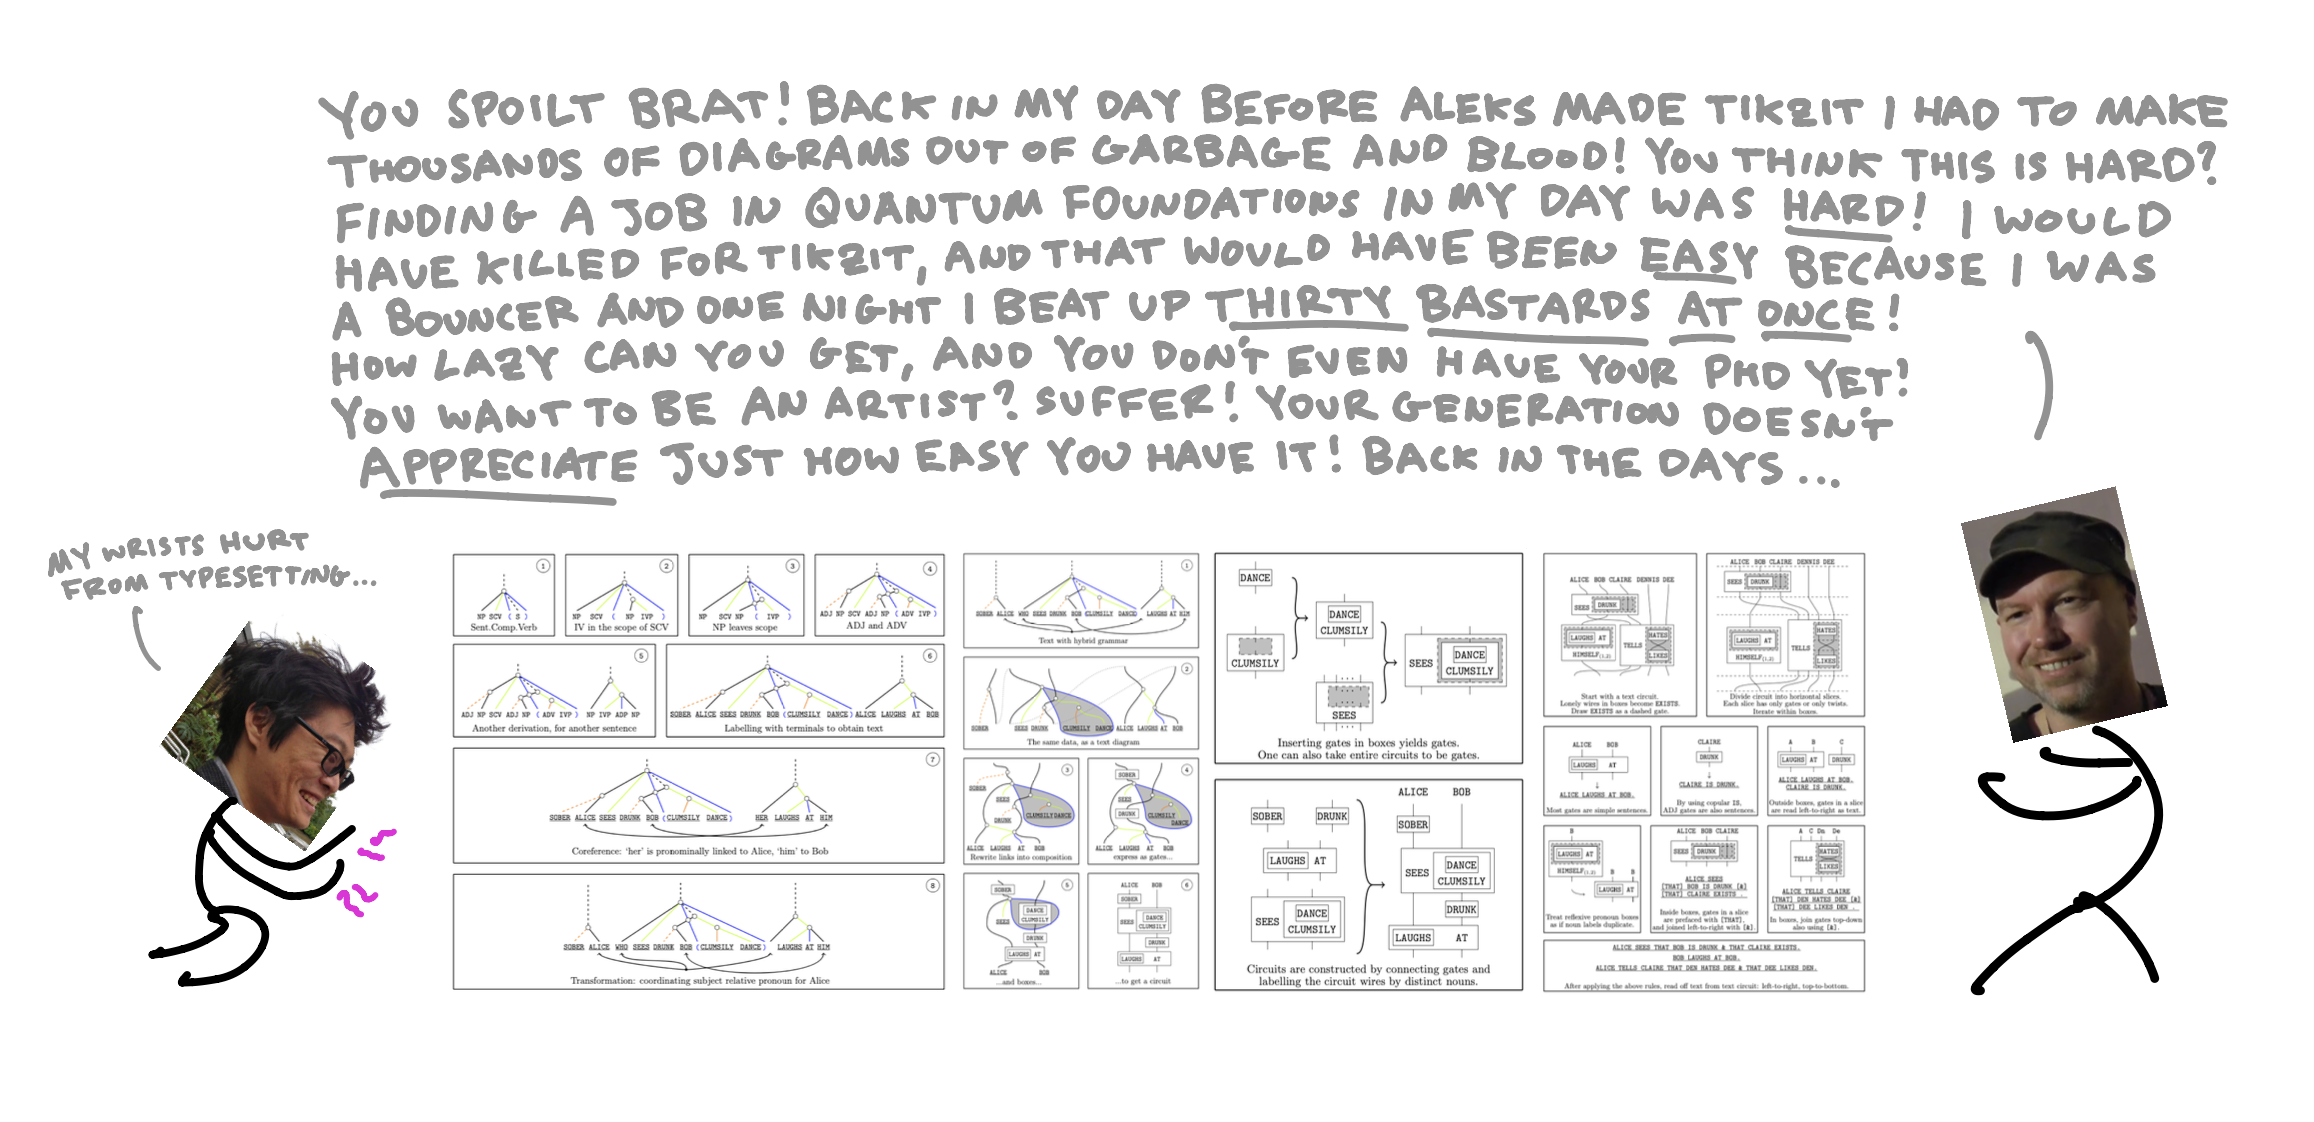
\includegraphics{figures/cartoons/bigpaper1}}
\caption{I realised that our intuitions were coming from an implicit productive grammar, rather than a parsing one, and that the path of least resistance for obtaining formal guarantees for the language-to-circuit procedure was to just handcraft a generative grammar for the fragment of language we were interested in. This meant scrapping everything in the first draft and starting again from scratch. Bob always had a word of gentle encouragement, giving me the motivation to persevere.\\
\\

So now we had two ways to obtain text circuits. One from pregroups (which Jono had extended the technique for to CCGs in his master's thesis \bR CITE \e), and one from handcrafted productive grammars. Then came time for me to write my thesis. Three salient questions arose. Firstly, what is the relationship between these two ways of getting at text circuits? Secondly, how do text circuits stand in relation to other generative grammars? Thirdly, what is it that text circuits allow us to do?\\ \\

These questions are now what the rest of the thesis seeks to answer.
}
\end{figure}